\addcontentsline{toc}{chapter}{Simulado 1}
\markboth{Simulado 1}{}

\num{1} Durante sua aula, Gabriel estava aprendendo a montar números utilizando o
material dourado e montou o seguinte número:

\begin{figure}[htpb!]
\centering
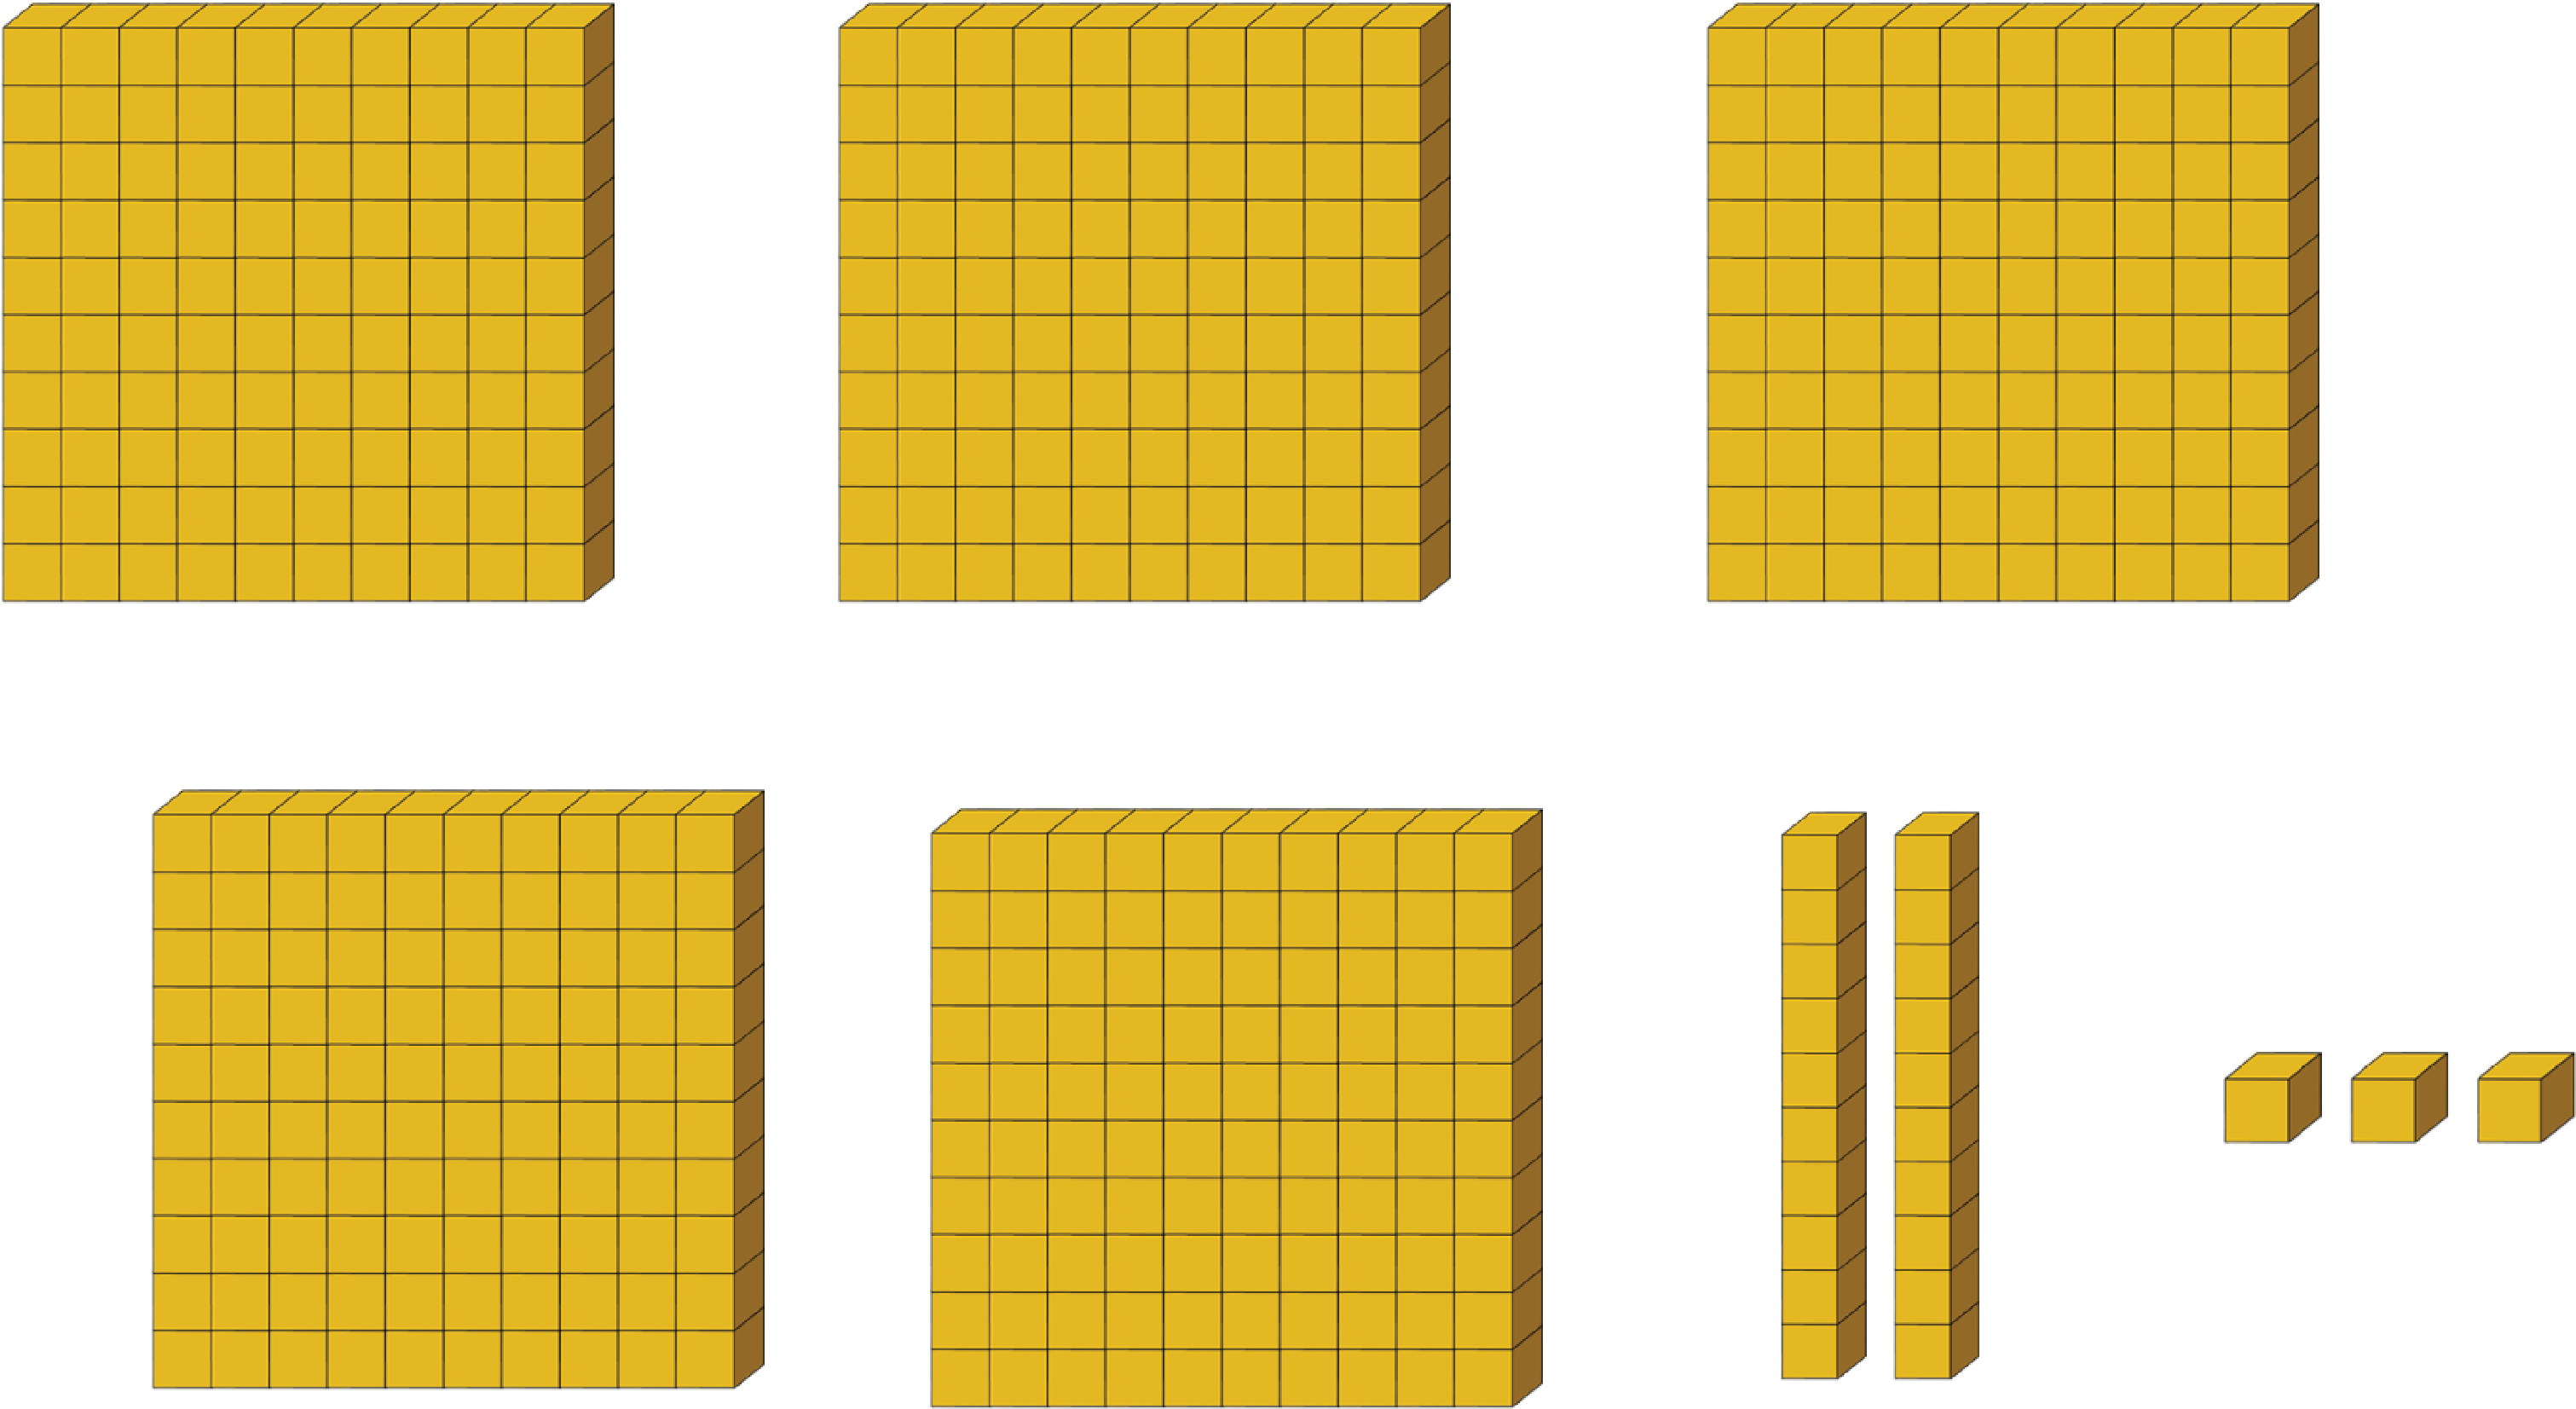
\includegraphics[width=\textwidth]{./media/image91.png}
\end{figure}

Qual é o número representado pelo material dourado na figura?

\begin{escolha}
\item
  623.
\item
  423.
\item
  503.
\item
  523.
\end{escolha}


\num{2} Alex estava jogando dardos em um alvo que possuía áreas de pontuação e
durante uma rodada notou que a expressão 2 x 1.000 + 3 x 100 + 1 x 10,
quando resolvida, gerava exatamente o número de pontos que ele havia
feito naquela rodada. A pontuação de Alex naquela rodada foi:

\begin{multicols}{2}
\begin{escolha}
\item
  231 pontos.
\item
  2.031 pontos.
\item
  2.301 pontos.
\item
  2.310 pontos.
\end{escolha}
\end{multicols}

\pagebreak
\num{3} José comprou uma linda placa com o número de sua casa.

\begin{figure}[htpb!]
\centering
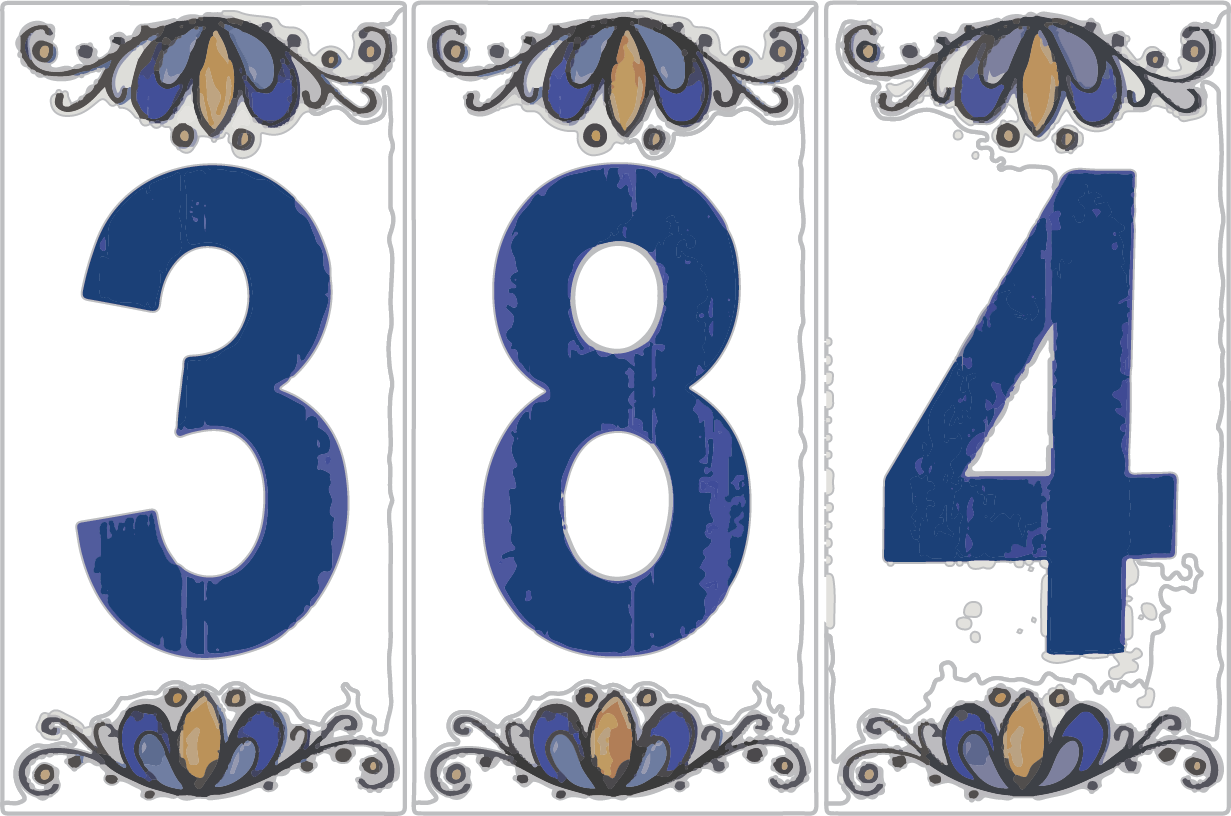
\includegraphics[width=.3\textwidth]{./media/image92.png}
\end{figure}


Porém, na hora de efetuar a compra, não percebeu que o número
estava errado, já que o primeiro e o último algarismos estão nas posi-
ções trocadas. Qual o valor relativo do último algarismo na placa e qual é o valor relativo no número da casa de José?

\begin{escolha}
\item
  Como está: 4; Como deveria ser: 40.
\item
  Como está: 40; Como deveria ser: 400.
\item
  Como está: 4; Como deveria ser: 400.
\item
  Como está: 40; Como deveria ser: 4.
\end{escolha}


\num{4} A escola em que Jack estuda está chamando a atenção para a importância do meio ambiente, promovendo uma ação educativa que consiste no plantio de mudas de árvores
nativas. Sabe-se que já foram plantadas 359 mudas e ainda serão
plantadas 246. Quantas mudas ao todo serão plantadas durante esse evento
da escola de Jack?

\begin{escolha}
\item
  513.
\item
  523.
\item
  605.
\item
  705.
\end{escolha}

\num{5} Na escola em que André estuda há 4.054 alunos. Já na escola em que
Pedro estuda estão matriculados 2.843 alunos. Se, no próximo ano, 300
alunos se matricularem em cada uma das escolas, qual será a diferença
entre a quantidade de alunos das duas escolas?

\begin{escolha}
\item
  2.422.
\item
  1.211.
\item
  1.883.
\item
  1.463.
\end{escolha}

\num{6} A numeração das salas de um novo prédio comercial de 5 andares segue a
numeração dos andares com a orientação da árvore que se localiza ao
lado do prédio. Assim, em cada andar a numeração começa pela sala mais
próxima da árvore, da seguinte maneira: 101, 102, 103, 201 etc.

\begin{figure}[htpb!]
\centering
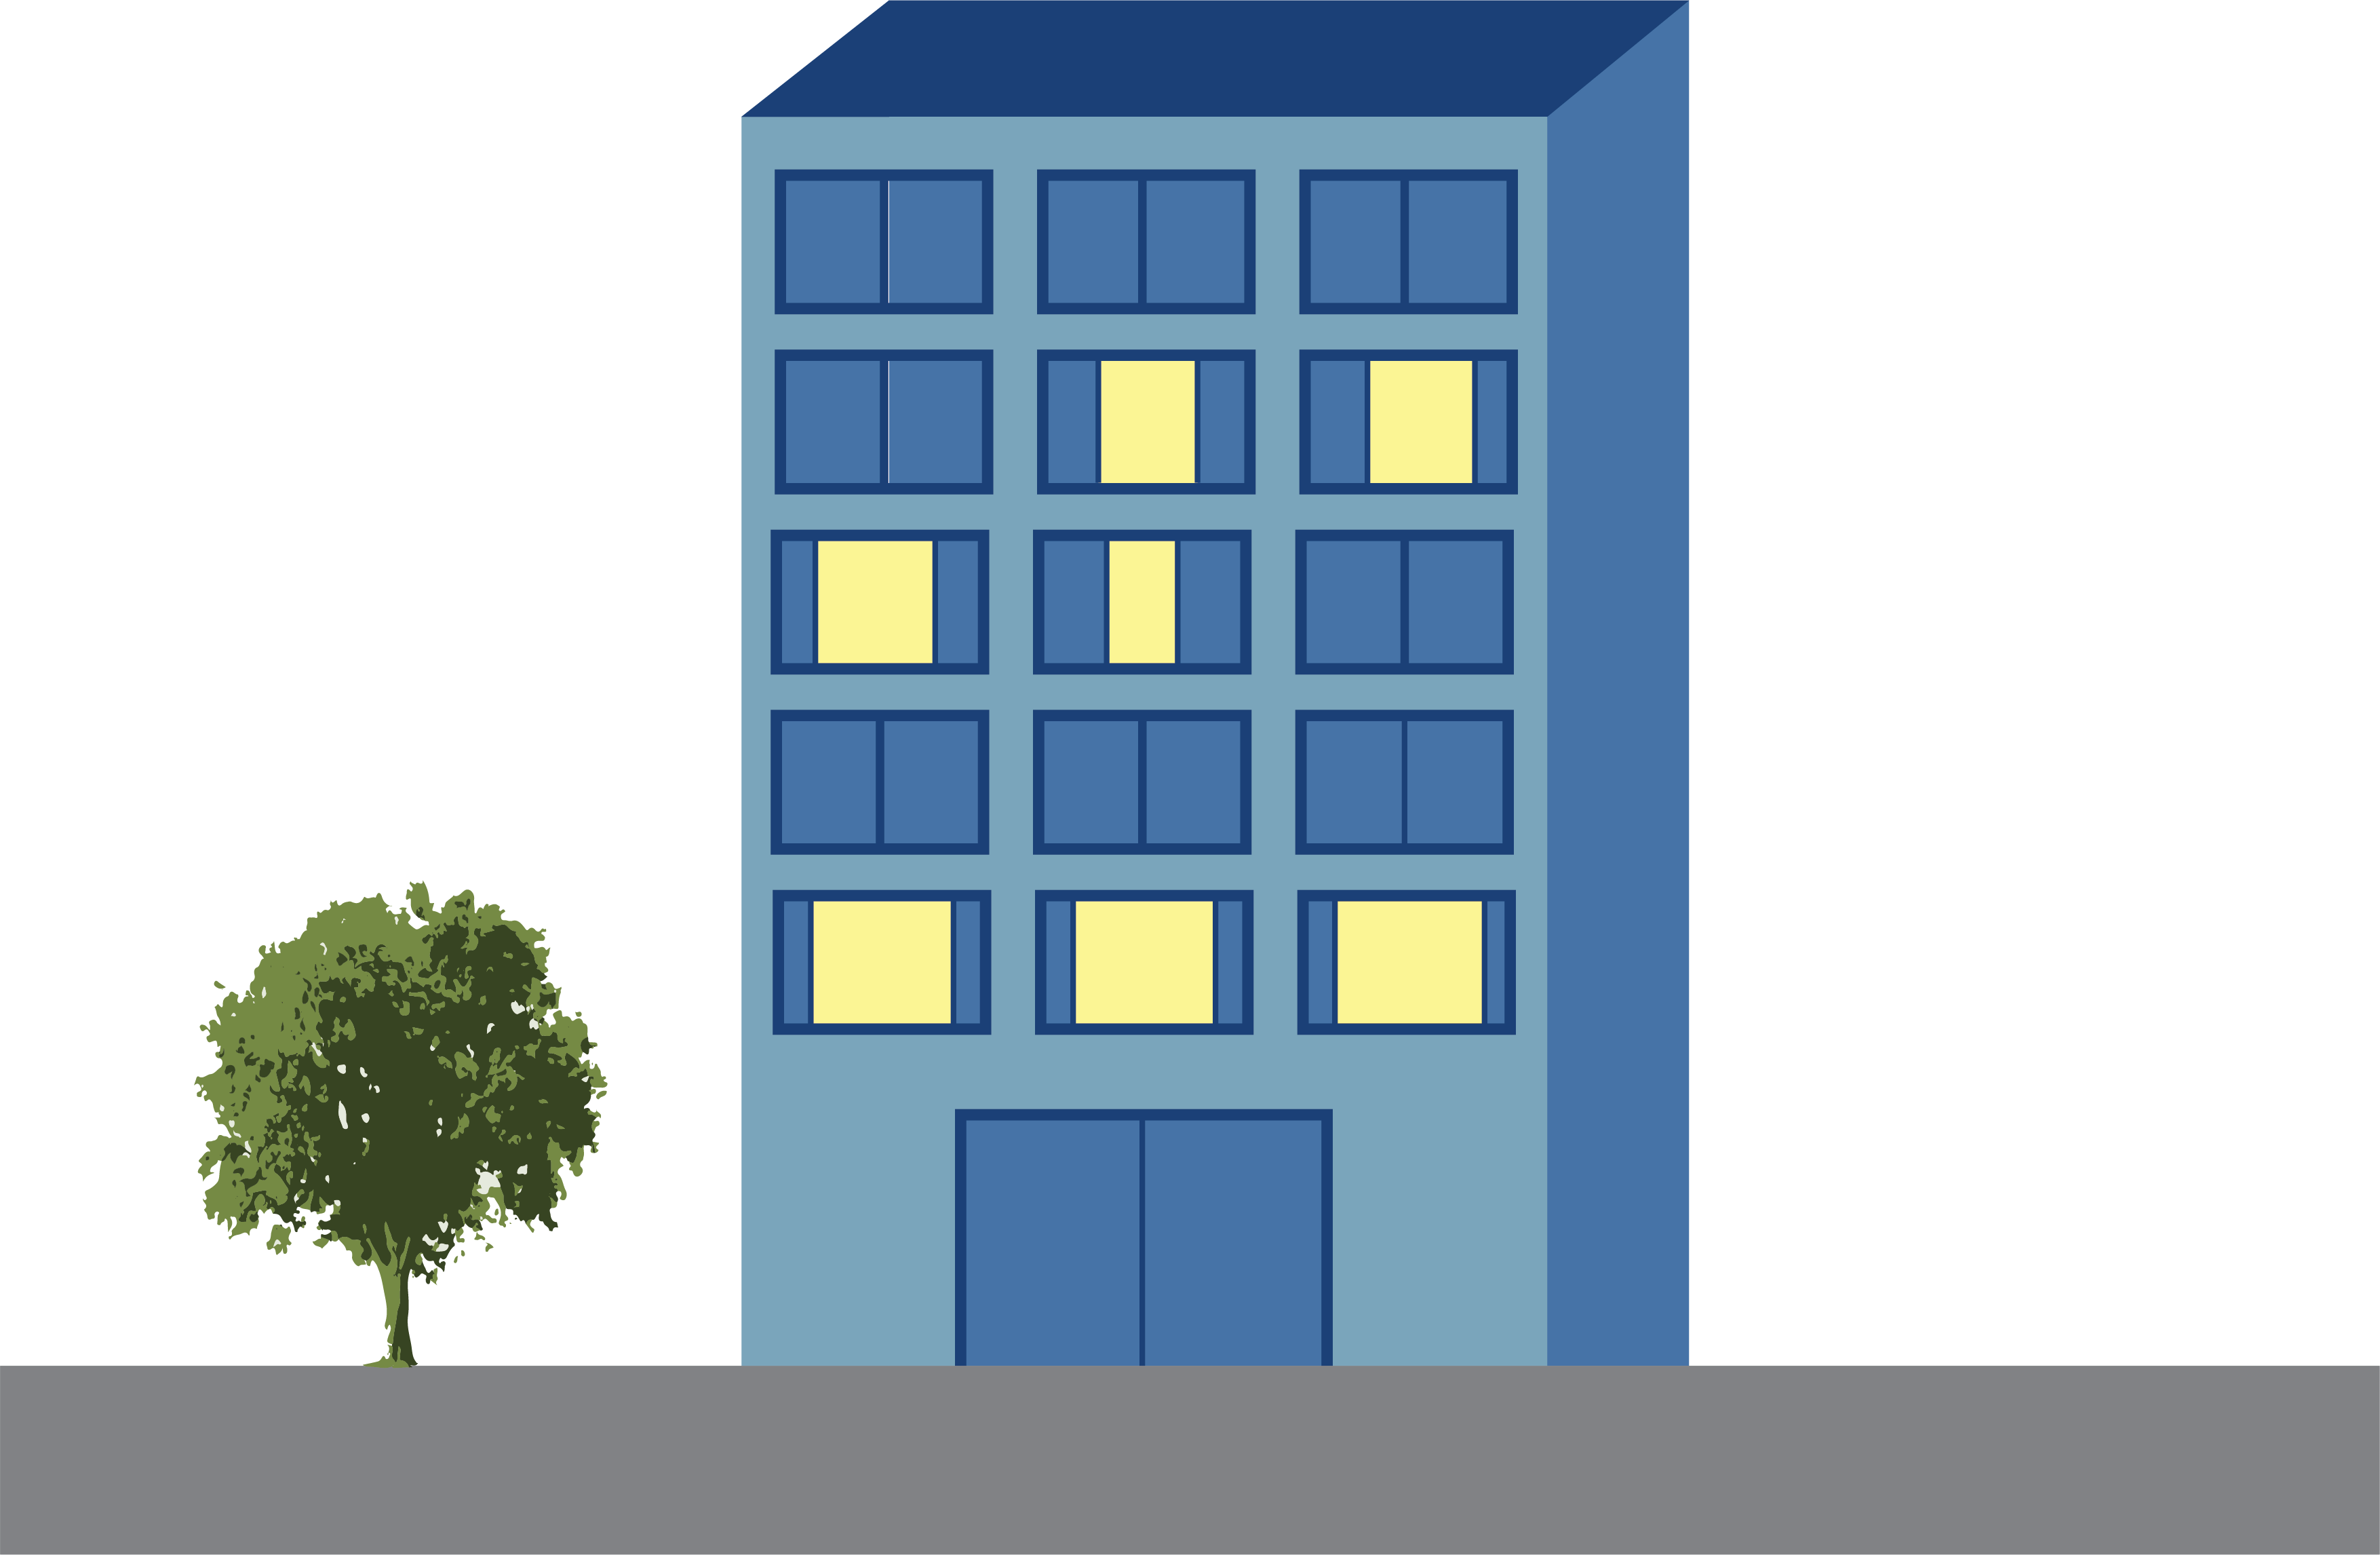
\includegraphics[width=.5\textwidth]{./media/image93.png}
\end{figure}

Qual a numeração da sala do 3º andar que está com a janela fechada?

\begin{escolha}
\item
  301.
\item
  302.
\item
  303.
\item
  304.
\end{escolha}

\num{7} Raquel está jogando um determinado jogo de pontos com sua prima. Ela
tinha 42 pontos na primeira rodada, perdeu 14 na segunda rodada e ganhou
5 na terceira rodada. Podemos afirmar que, ao final da terceira rodada, Raquel estava com

\begin{escolha}
\item
  33 pontos.
\item
  37 pontos.
\item
  61 pontos.
\item
  5 pontos.
\end{escolha}

\num{8} Observe a figura.

\begin{figure}[htpb!]
\centering
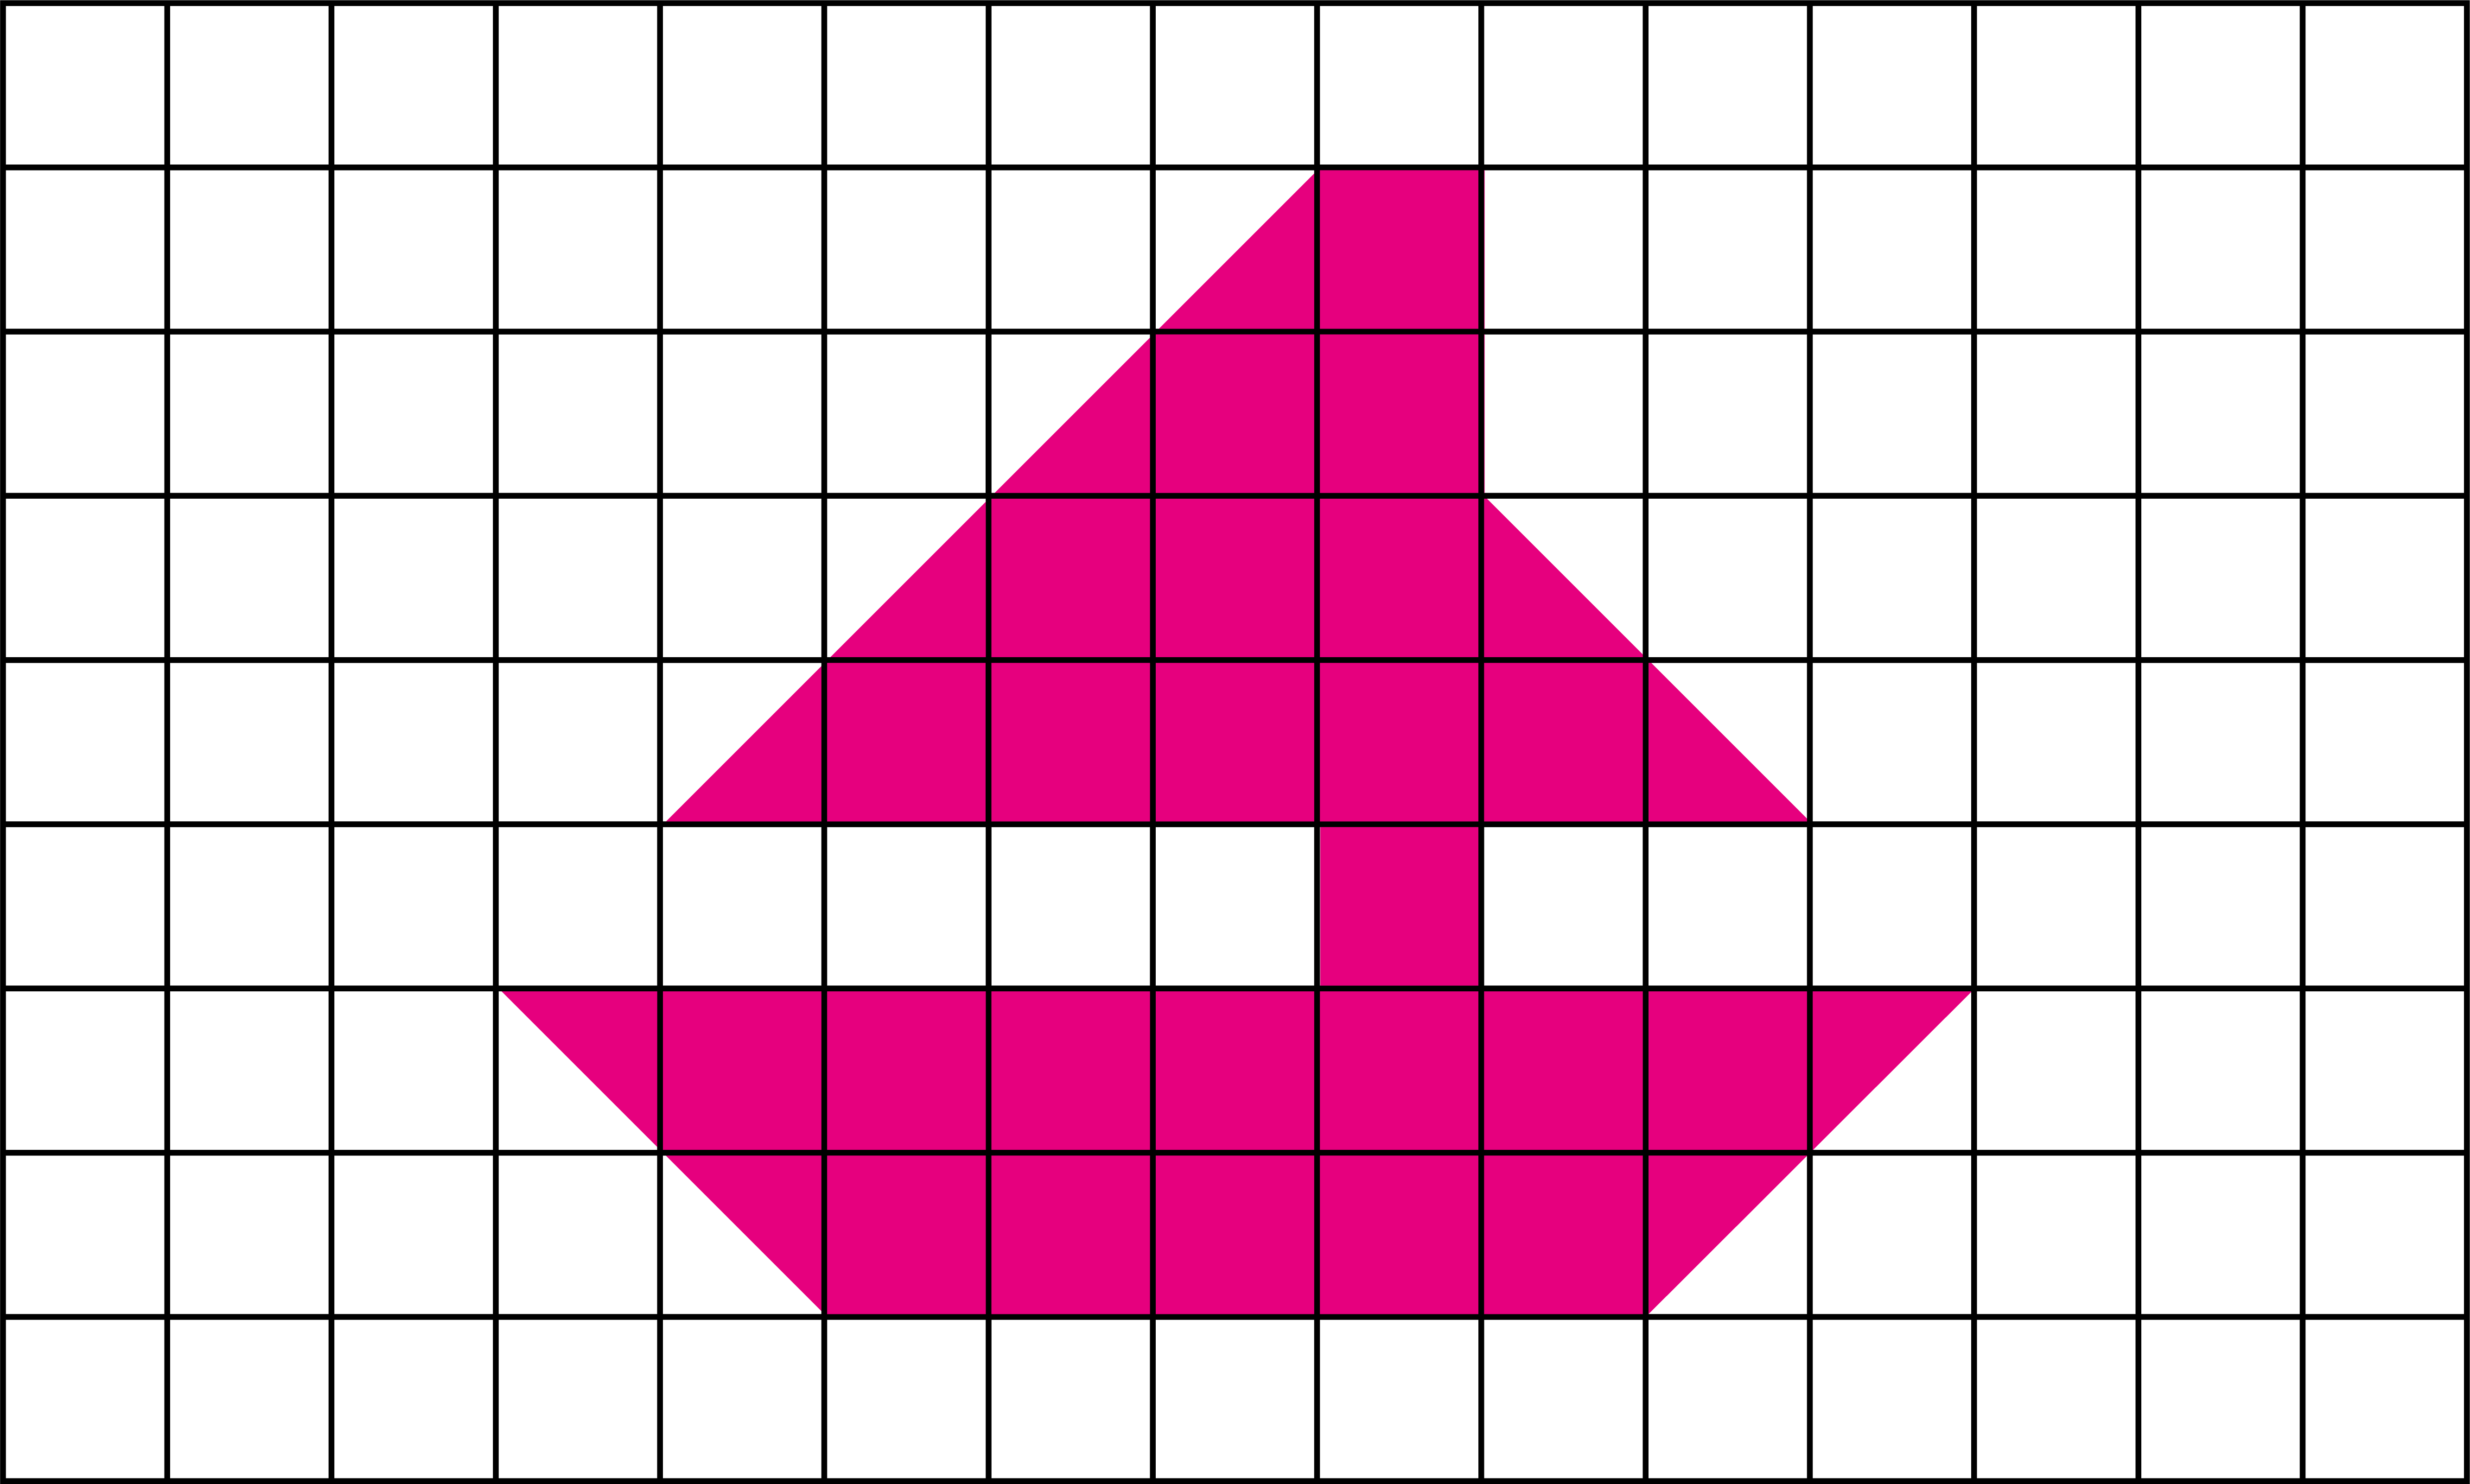
\includegraphics[width=.6\textwidth]{./media/image94.png}
\end{figure}

Considerando tudo o que está pintado e, se precisar, juntando pedaços
menores para formar quadrados, quantos quadrados estão pintados?

\begin{escolha}
\item
  24.
\item
  26.
\item
  29.
\item
  34.
\end{escolha}

\pagebreak
\num{9} Ana Beatriz e Camila juntaram todo o dinheiro que ganharam de seus pais no
último mês e as quantias estão representadas em uma figura.

\begin{figure}[htpb!]
\centering
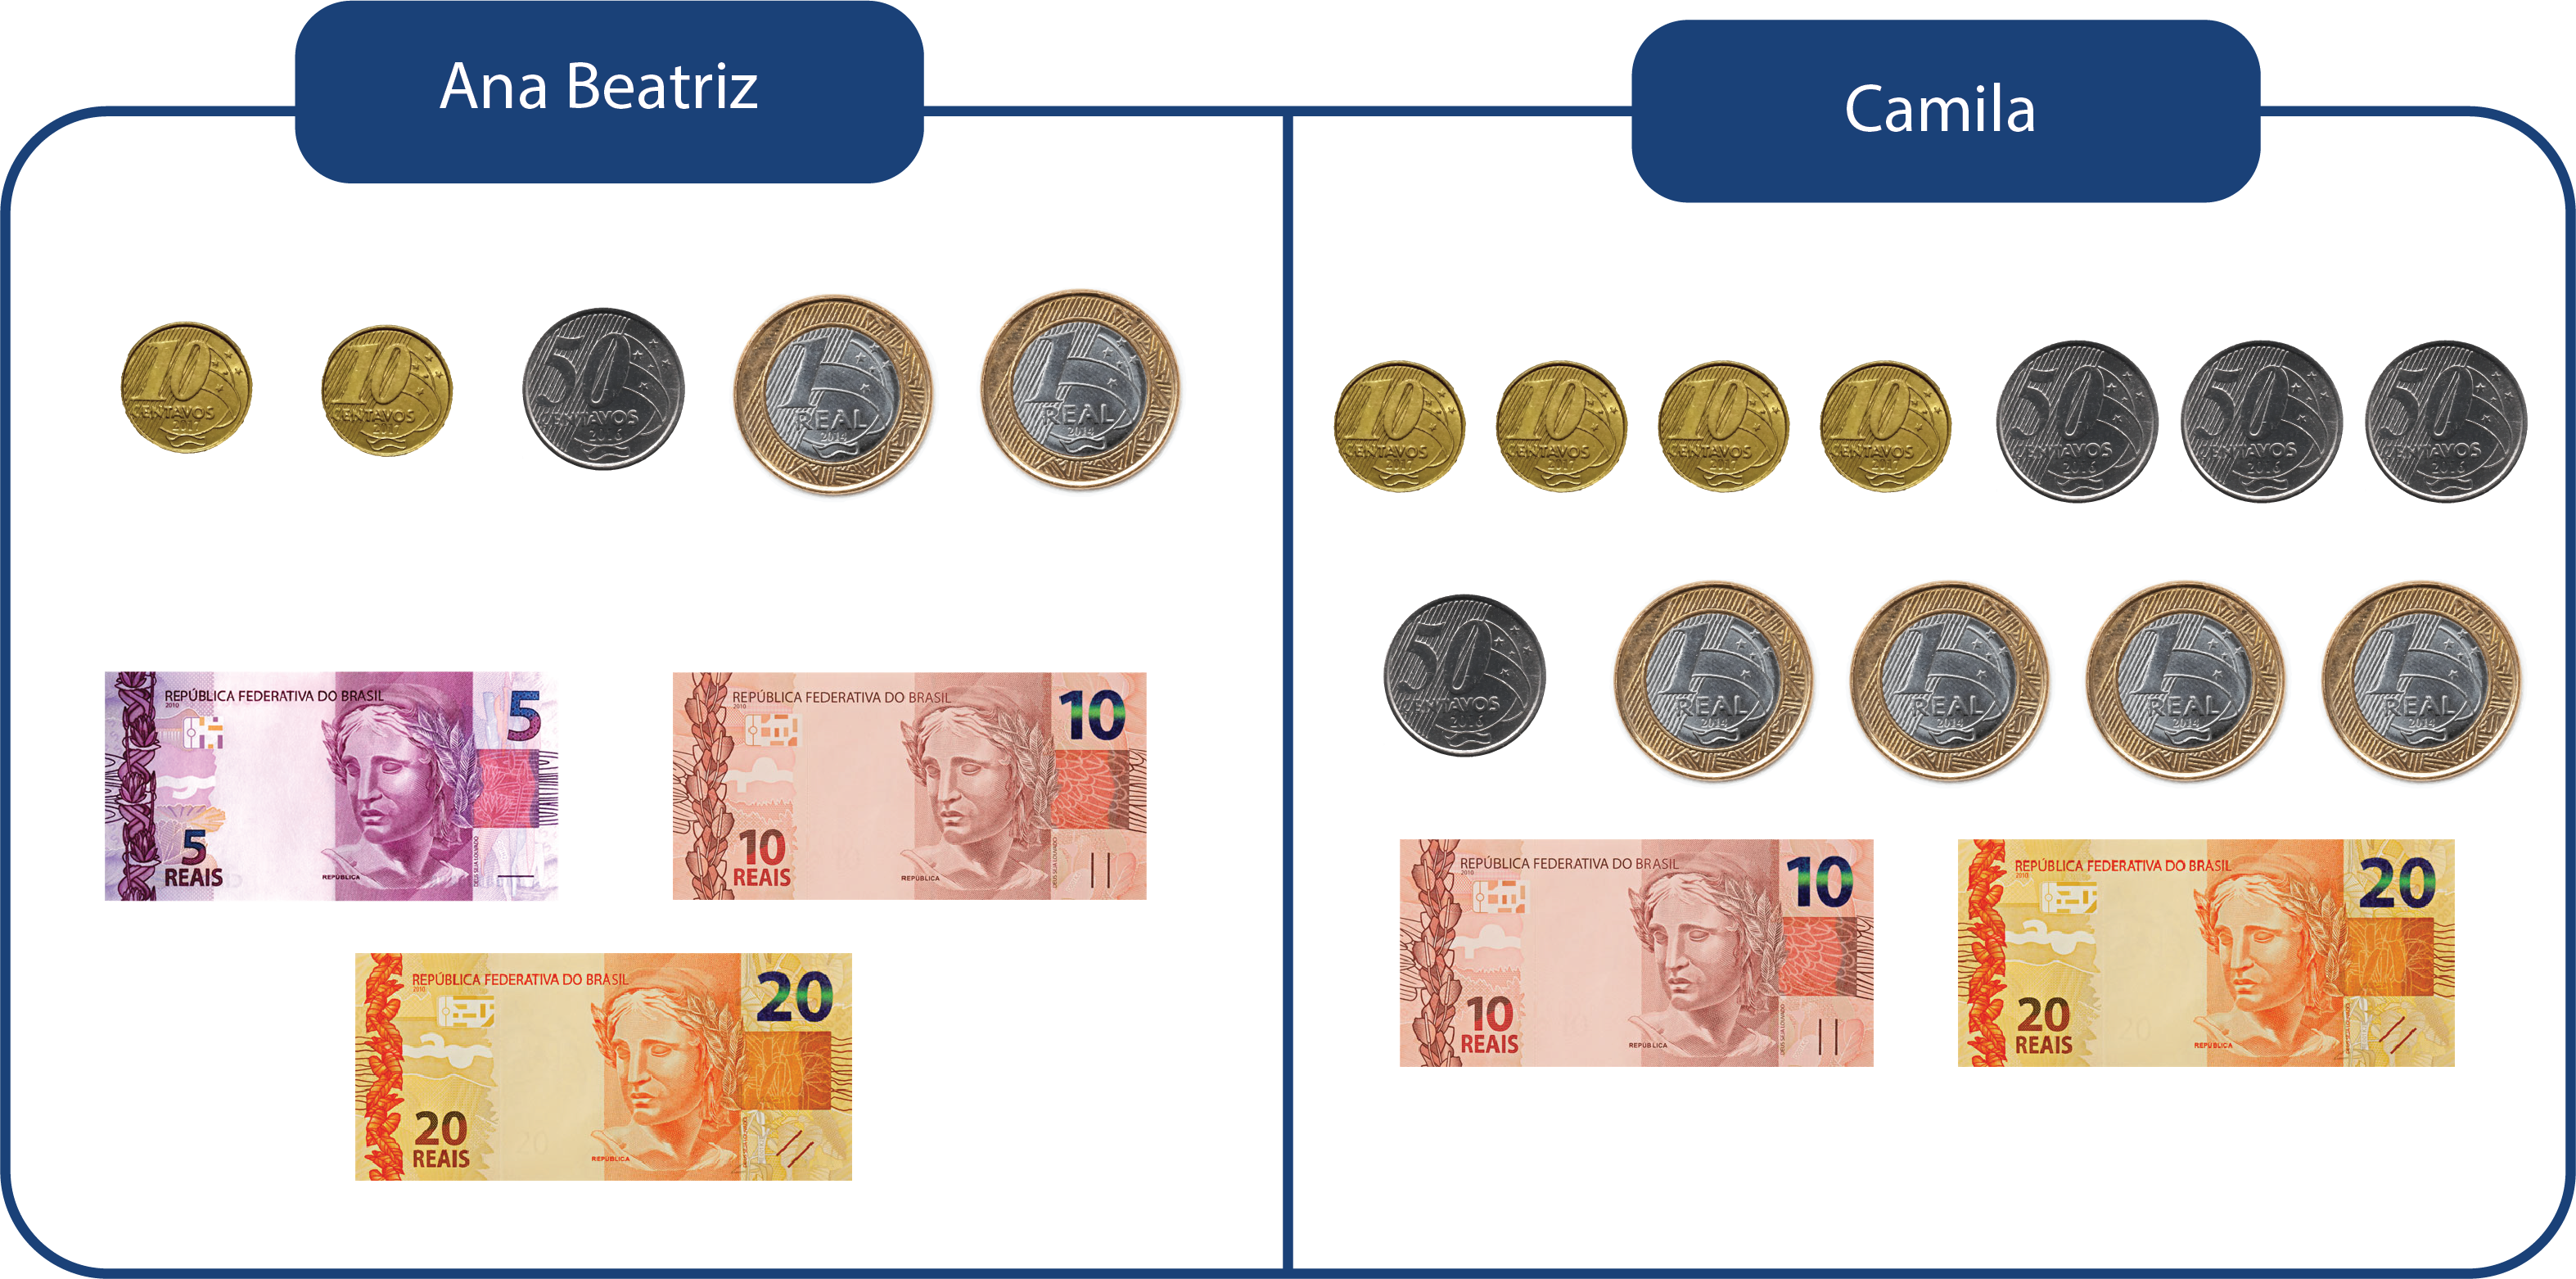
\includegraphics[width=0.6\textwidth]{./media/image95.png}
\end{figure}

Somando-se os dois valores, qual é o valor total que as duas conseguiram juntar?

\begin{multicols}{2}
\begin{escolha}
\item
  R\$ 36,40.
\item
  R\$ 37,70.
\item
  R\$ 74,10.
\item
  R\$ 85,20.
\end{escolha}
\end{multicols}

\num{10} Gabriel achou nas coisas guardadas de seu irmão mais velho a seguinte malha quadriculada com letras destacadas:

\begin{figure}[htpb!]
\centering
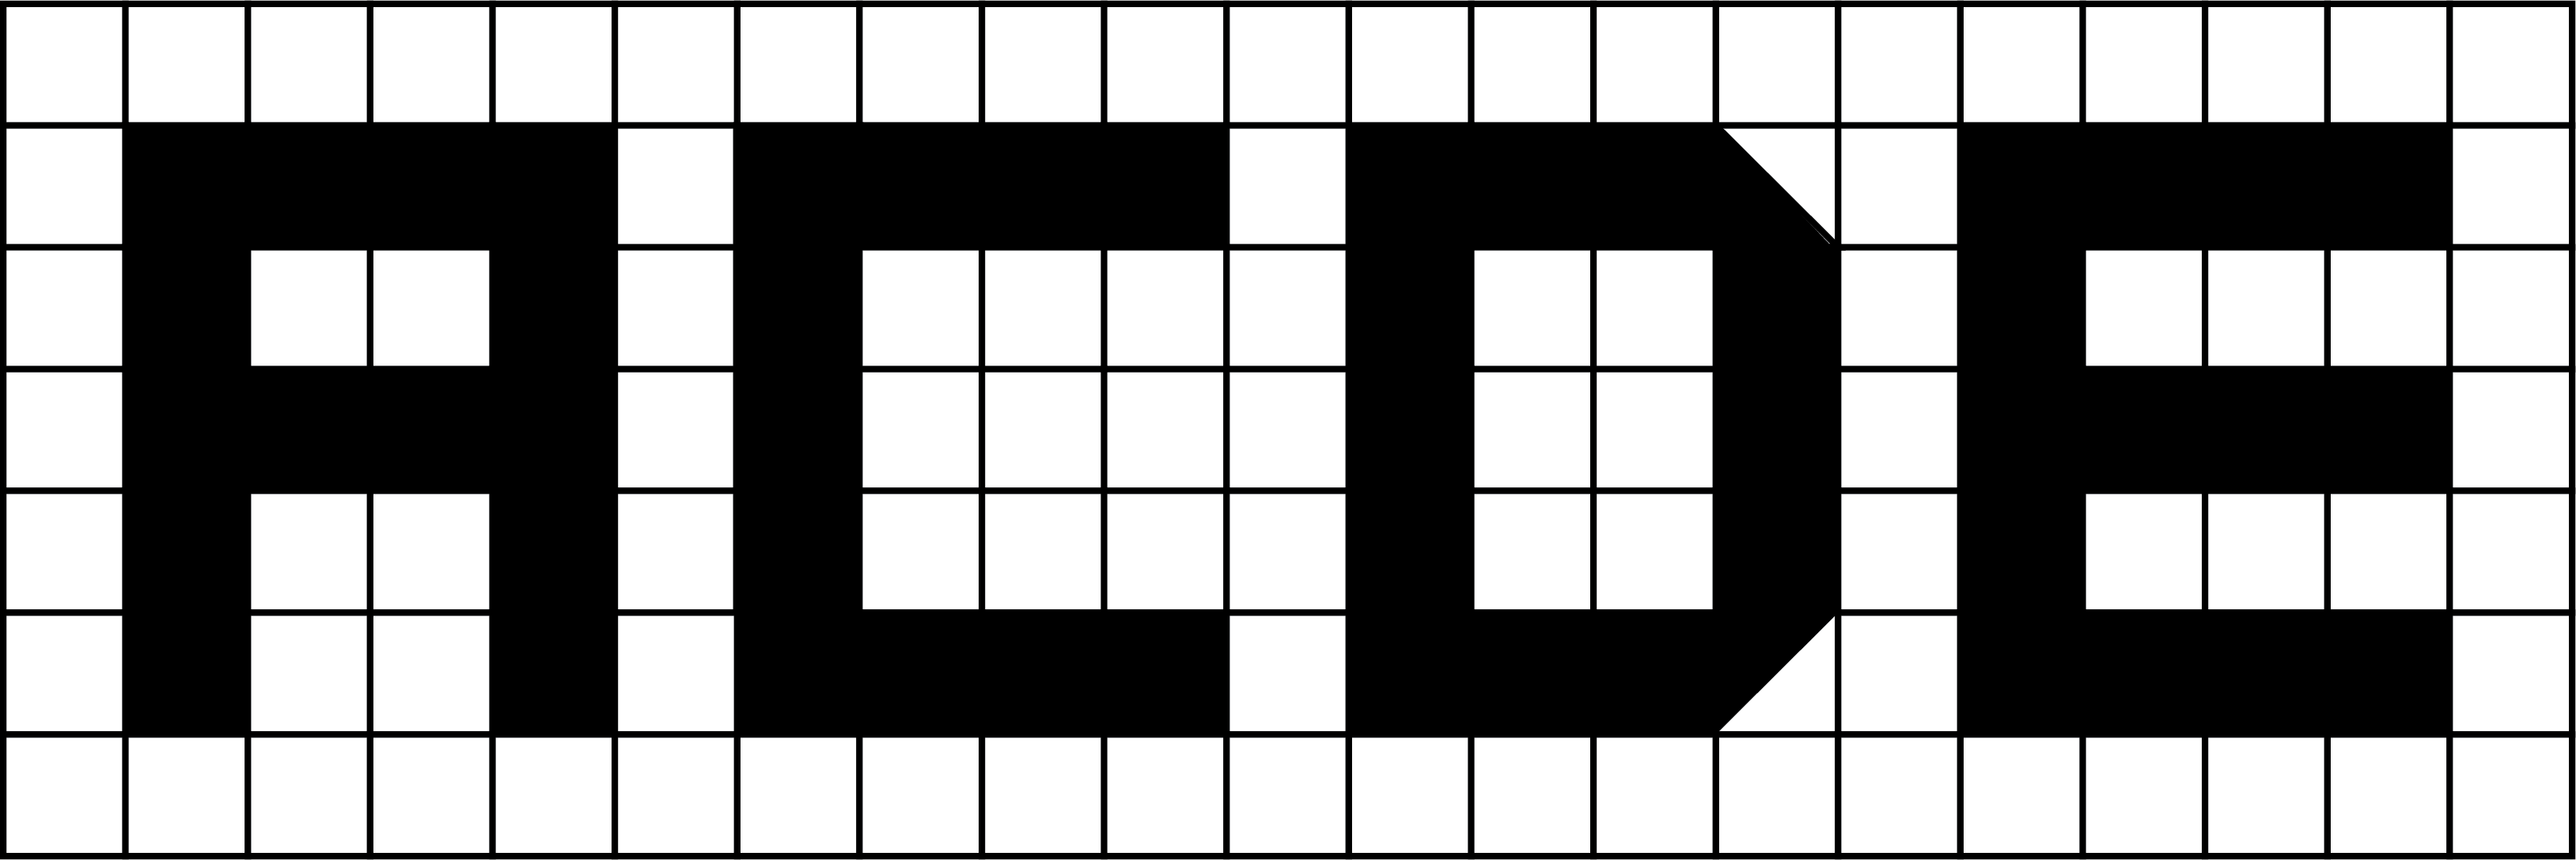
\includegraphics[width=0.5\textwidth]{./media/image96.png}
\end{figure}

Dentre elas, existem duas letras que usam o mesmo número de quadradinhos para serem formadas. Essas letras são

\begin{escolha}
\item
  A e C
\item
  D e E
\item
  D e C
\item
  A e E
\end{escolha}

\num{11} Uma escola fez um levantamento sobre a quantidade de alunos em dois anos
do ensino fundamental. Os dados foram apresentados em um gráfico.

\begin{figure}[htpb!]
\centering
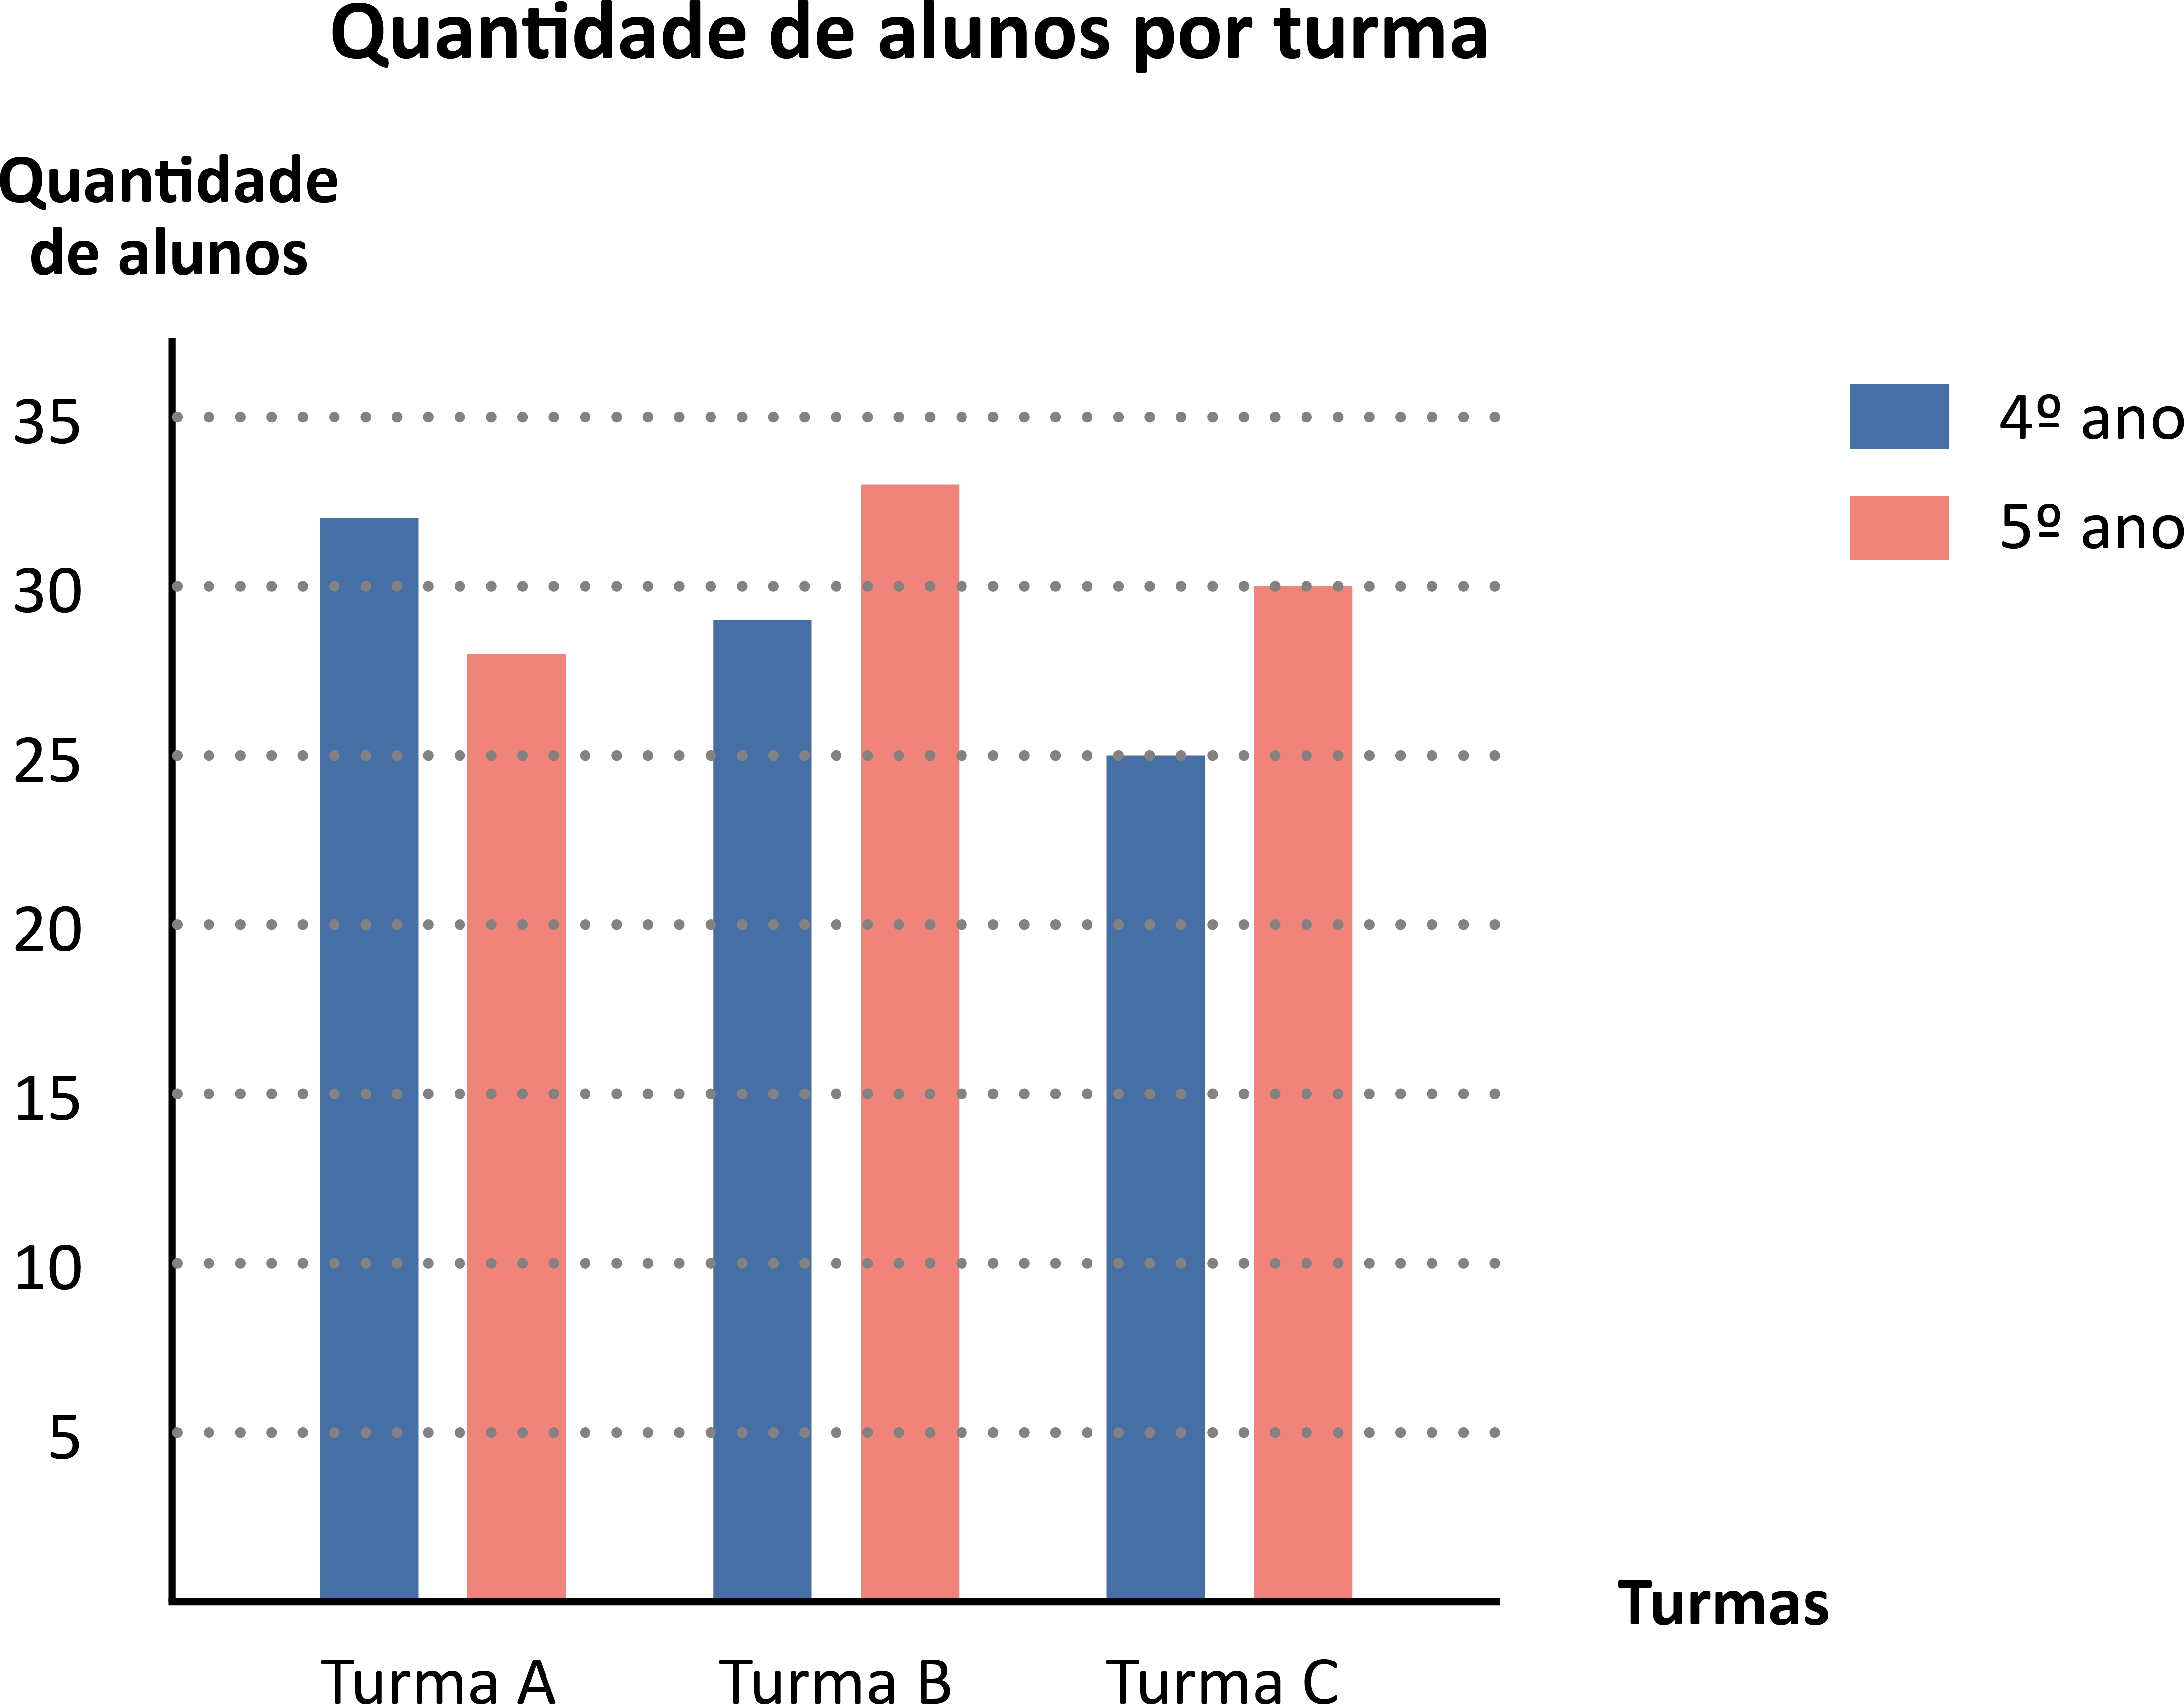
\includegraphics[width=\textwidth]{./media/image97.png}
\end{figure}

Após analisar o gráfico, calcule e assinale a alternativa que traz o número total de alunos do 4º ano.

%\begin{multicols}{2}
\begin{escolha}
\item
  60
\item
  86
\item
  91
\item
  150
\end{escolha}
%\end{multicols}

\pagebreak

\num{12} Assinale a alternativa que traz a sequência dos números dos balões ordenados de forma decrescente.

\begin{figure}[htpb!]
\centering
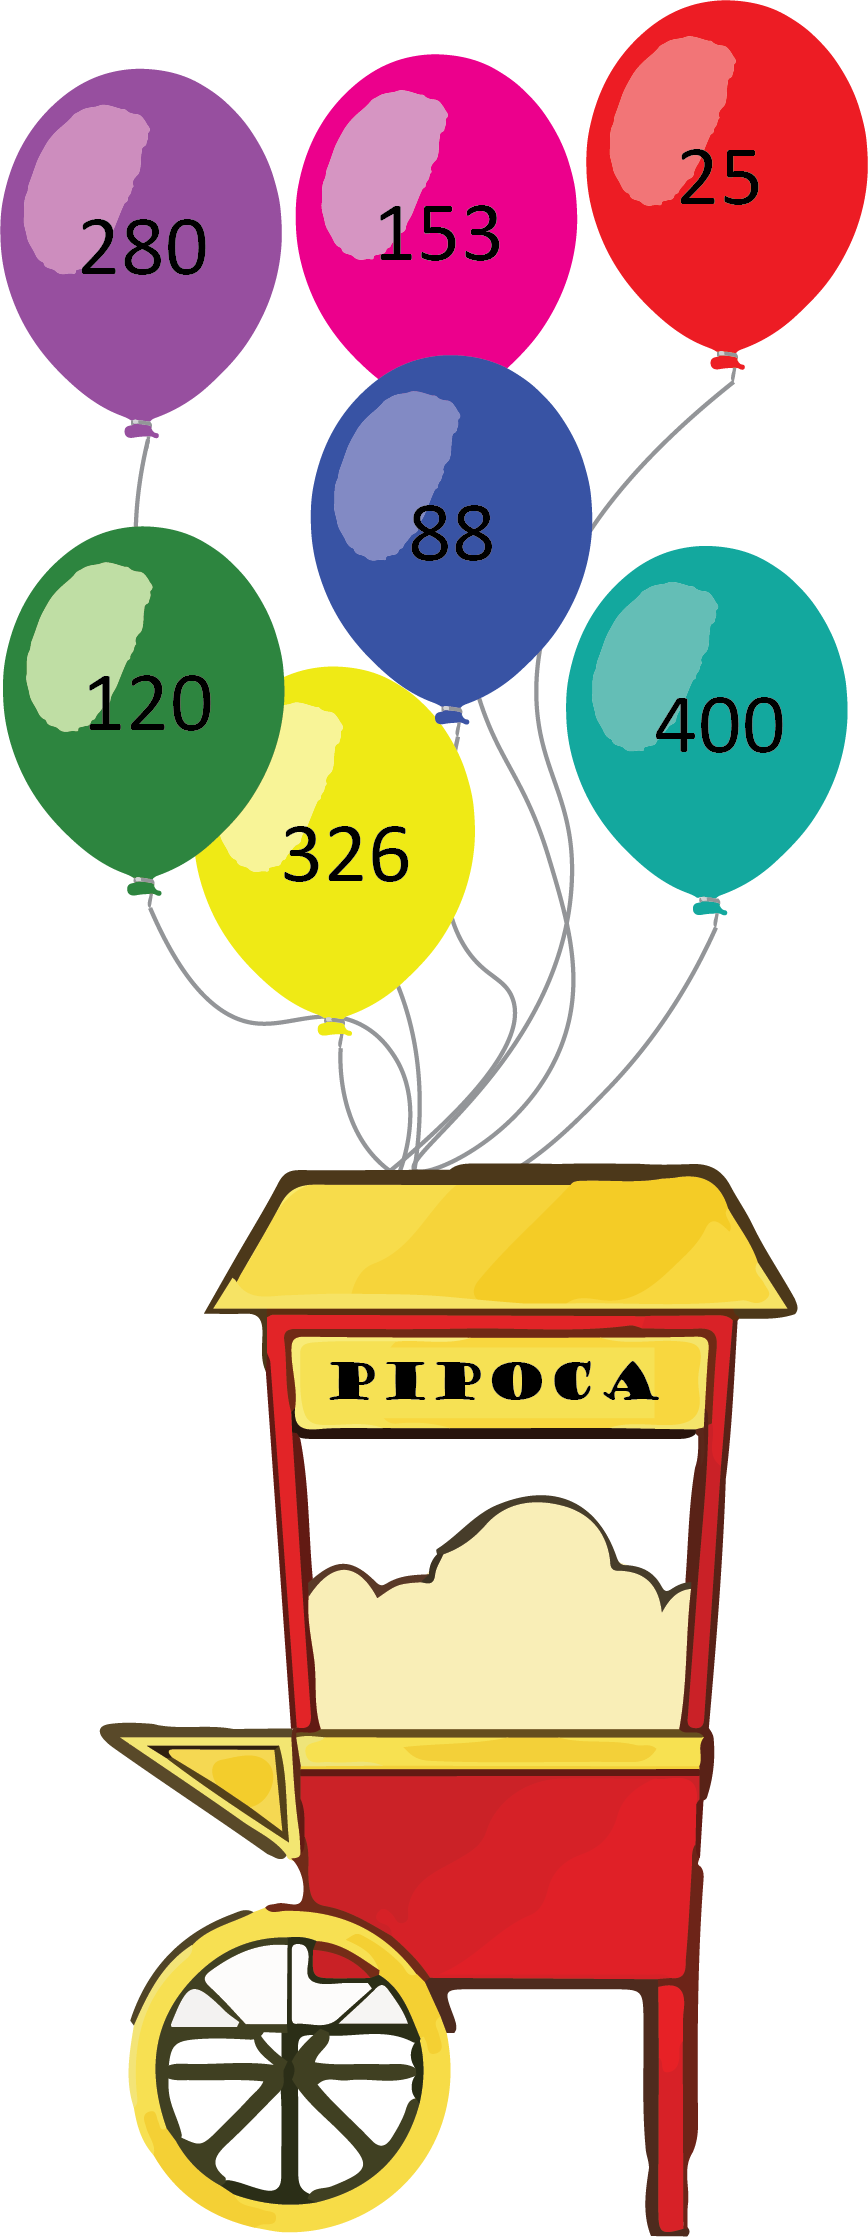
\includegraphics[width=.3\textwidth]{./media/image98.png}
\end{figure}

\begin{escolha}
\item
  (25; 88; 120; 153; 280; 326; 400)
\item
  (25; 120; 280; 88; 400; 153; 326)
\item
  (88; 25; 120; 280; 153; 326; 400)
\item
  (400; 326; 280; 153; 120; 88; 25)
\end{escolha}

\pagebreak

\num{13} A professora de Adriana pediu para que ela fosse até a lousa e resolvesse a seguinte conta:

\begin{figure}[htpb!]
\centering
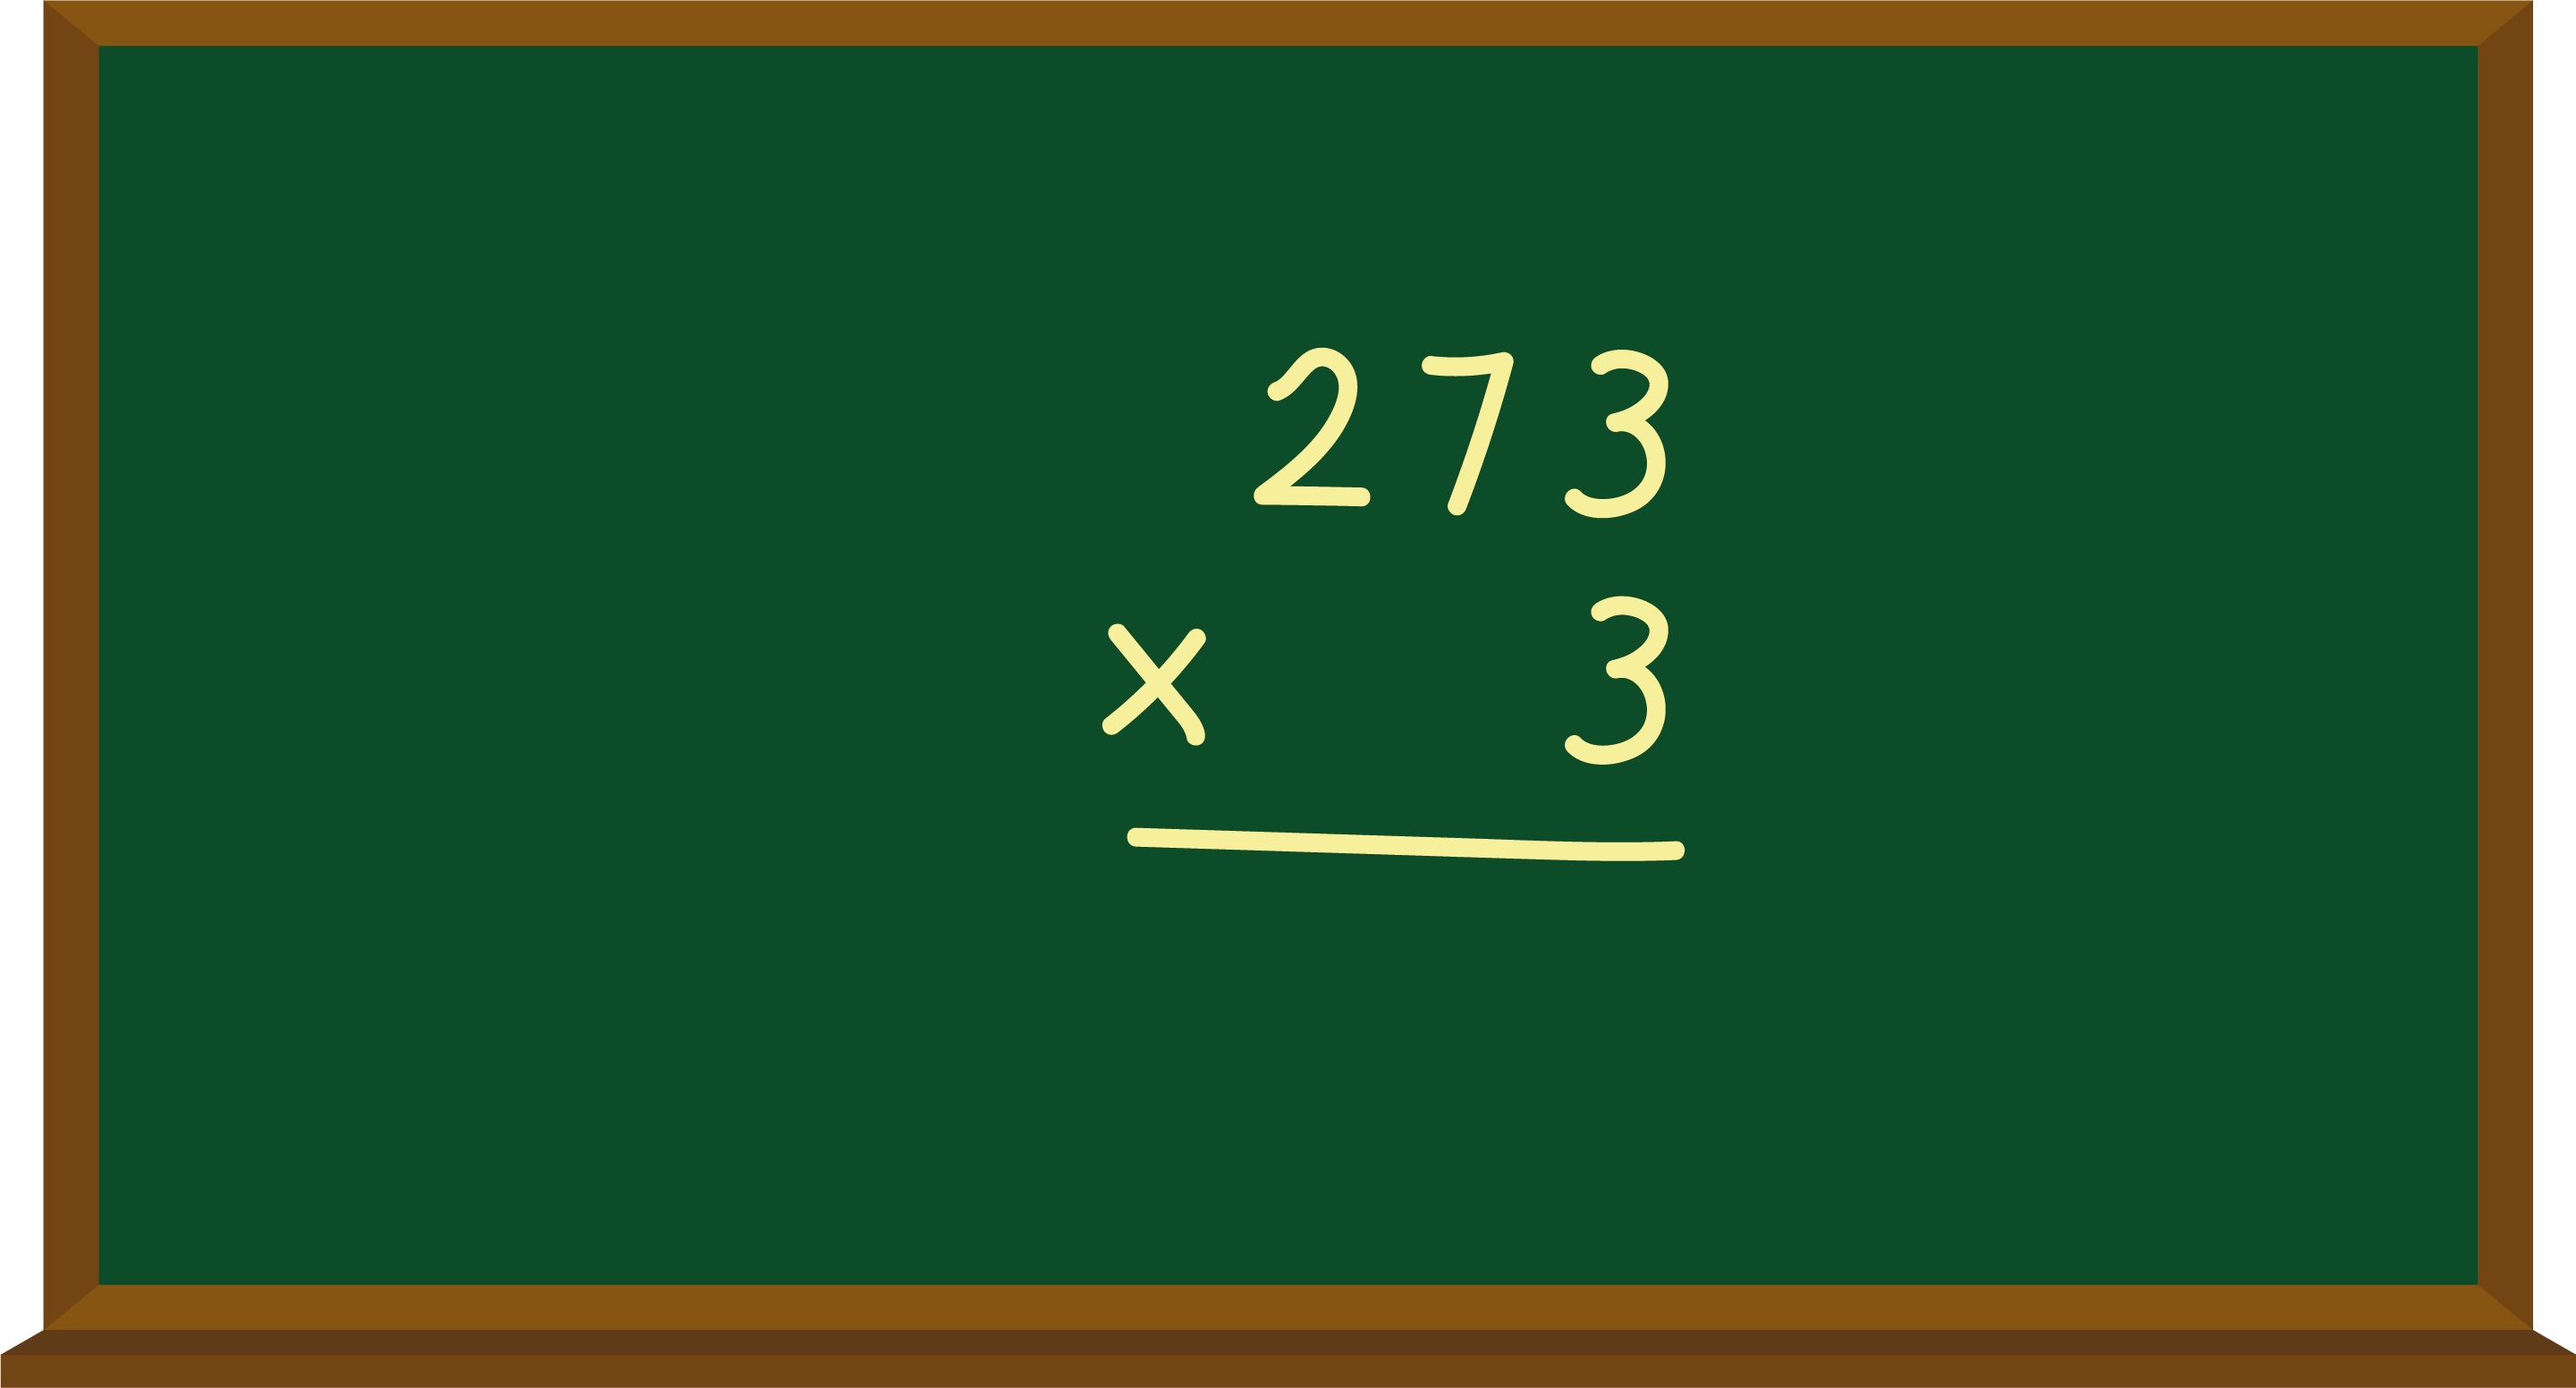
\includegraphics[width=0.7\textwidth]{./media/image99.png}
\end{figure}

Ajude Adriana a resolver essa conta identificando a alternativa que traz a resposta correta.

\begin{multicols}{2}
\begin{escolha}
\item
  819
\item
  625
\item
  546
\item
  273
\end{escolha}
\end{multicols}


\num{14} O relógio de parede do consultório médico em que Graziela está esperando
para ser atendida está com os ponteiros posicionados da seguinte maneira:

\begin{figure}[htpb!]
\centering
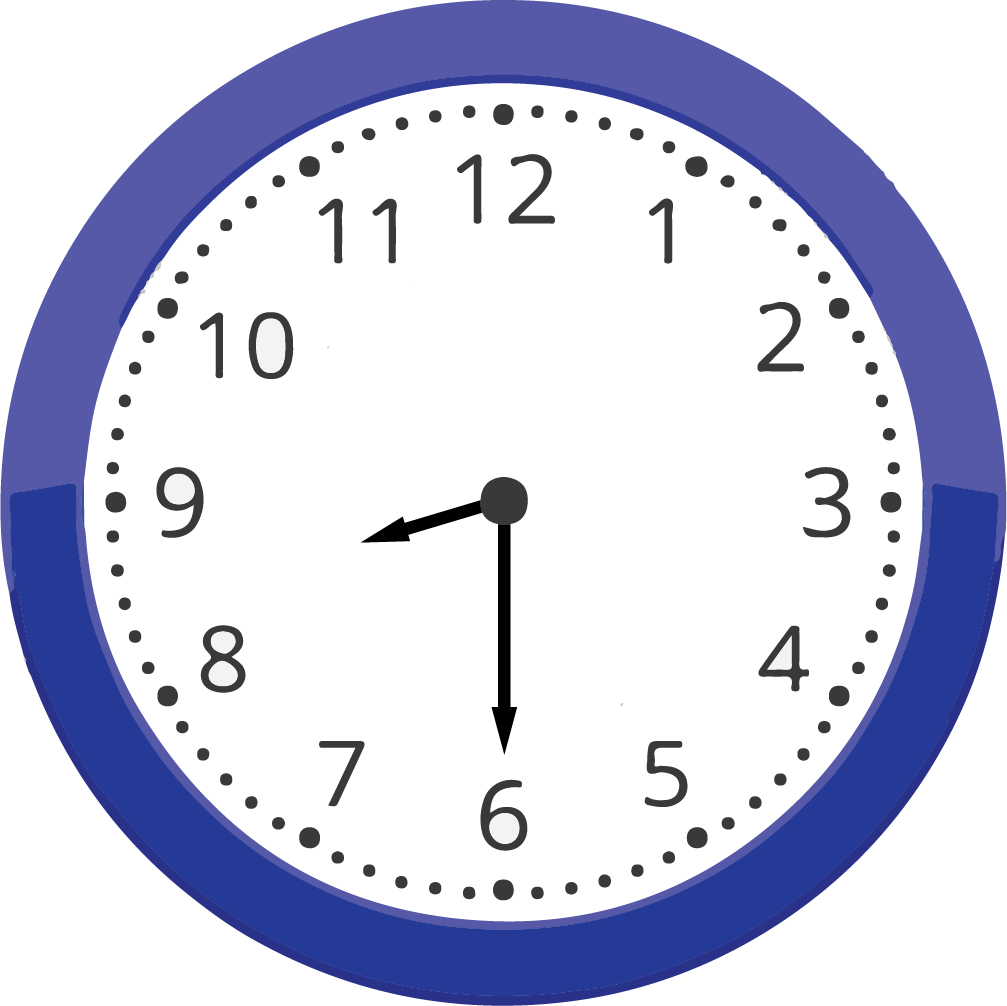
\includegraphics[width=.4\textwidth]{./media/image100.png}
\end{figure}

Assinale a alternativa que mostra a hora representada no relógio da imagem.

\begin{escolha}
\item
  8 horas e 30 minutos.
\item
  7 horas e 15 minutos.
\item
  8 horas e 50 minutos.
\item
  7 horas e 50 minutos.
\end{escolha}


\num{15} Observe a imagem. Ela apresenta uma comparação entre o tamanho de dois lápis.

\begin{figure}[htpb!]
\centering
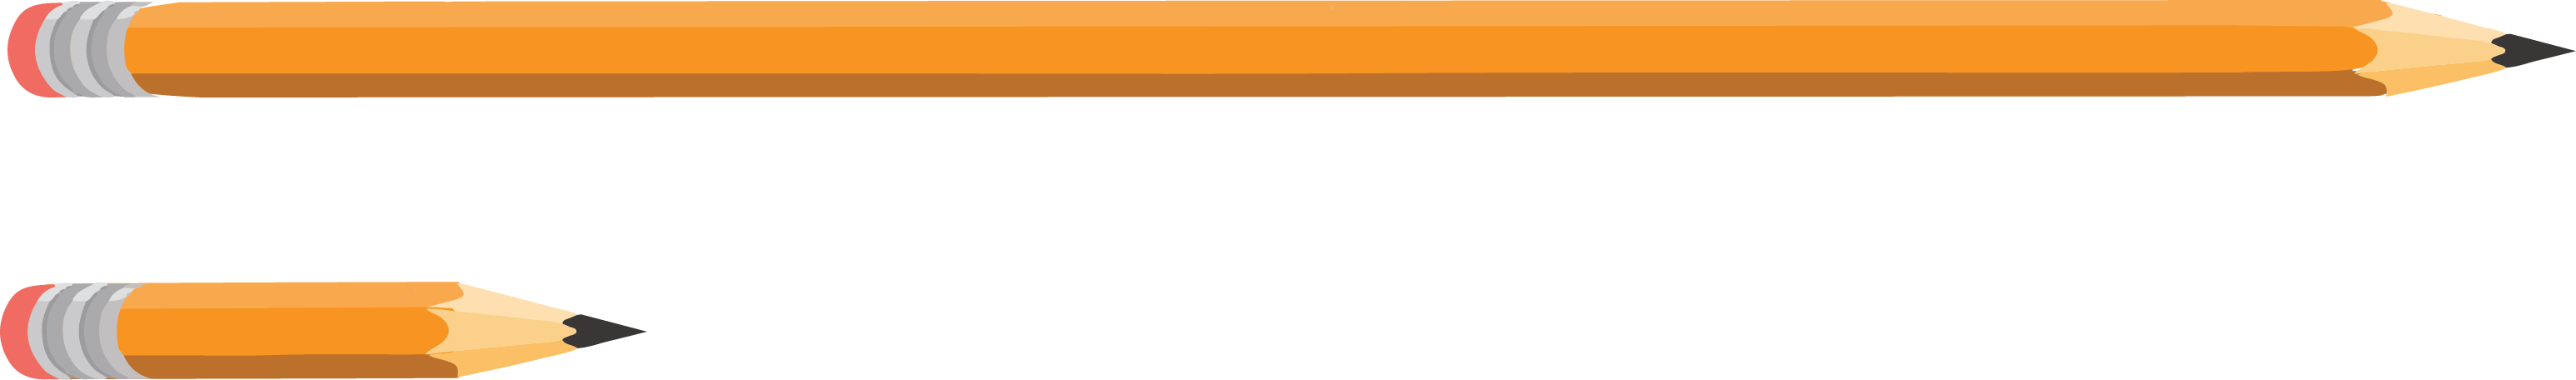
\includegraphics[width=\textwidth]{./media/image101.png}
\end{figure}

Pela observação, pode-se afirmar que o lápis maior mede aproximadamente

\begin{escolha}
\item
  Duas vezes o lápis menor.
\item
  Quatro vezes o lápis menor.
\item
  Dez vezes o lápis menor.
\item
  Uma vez o lápis menor.
\end{escolha}
\pagebreak

\vspace*{-3.4cm}
%\hspace*{-3.7cm}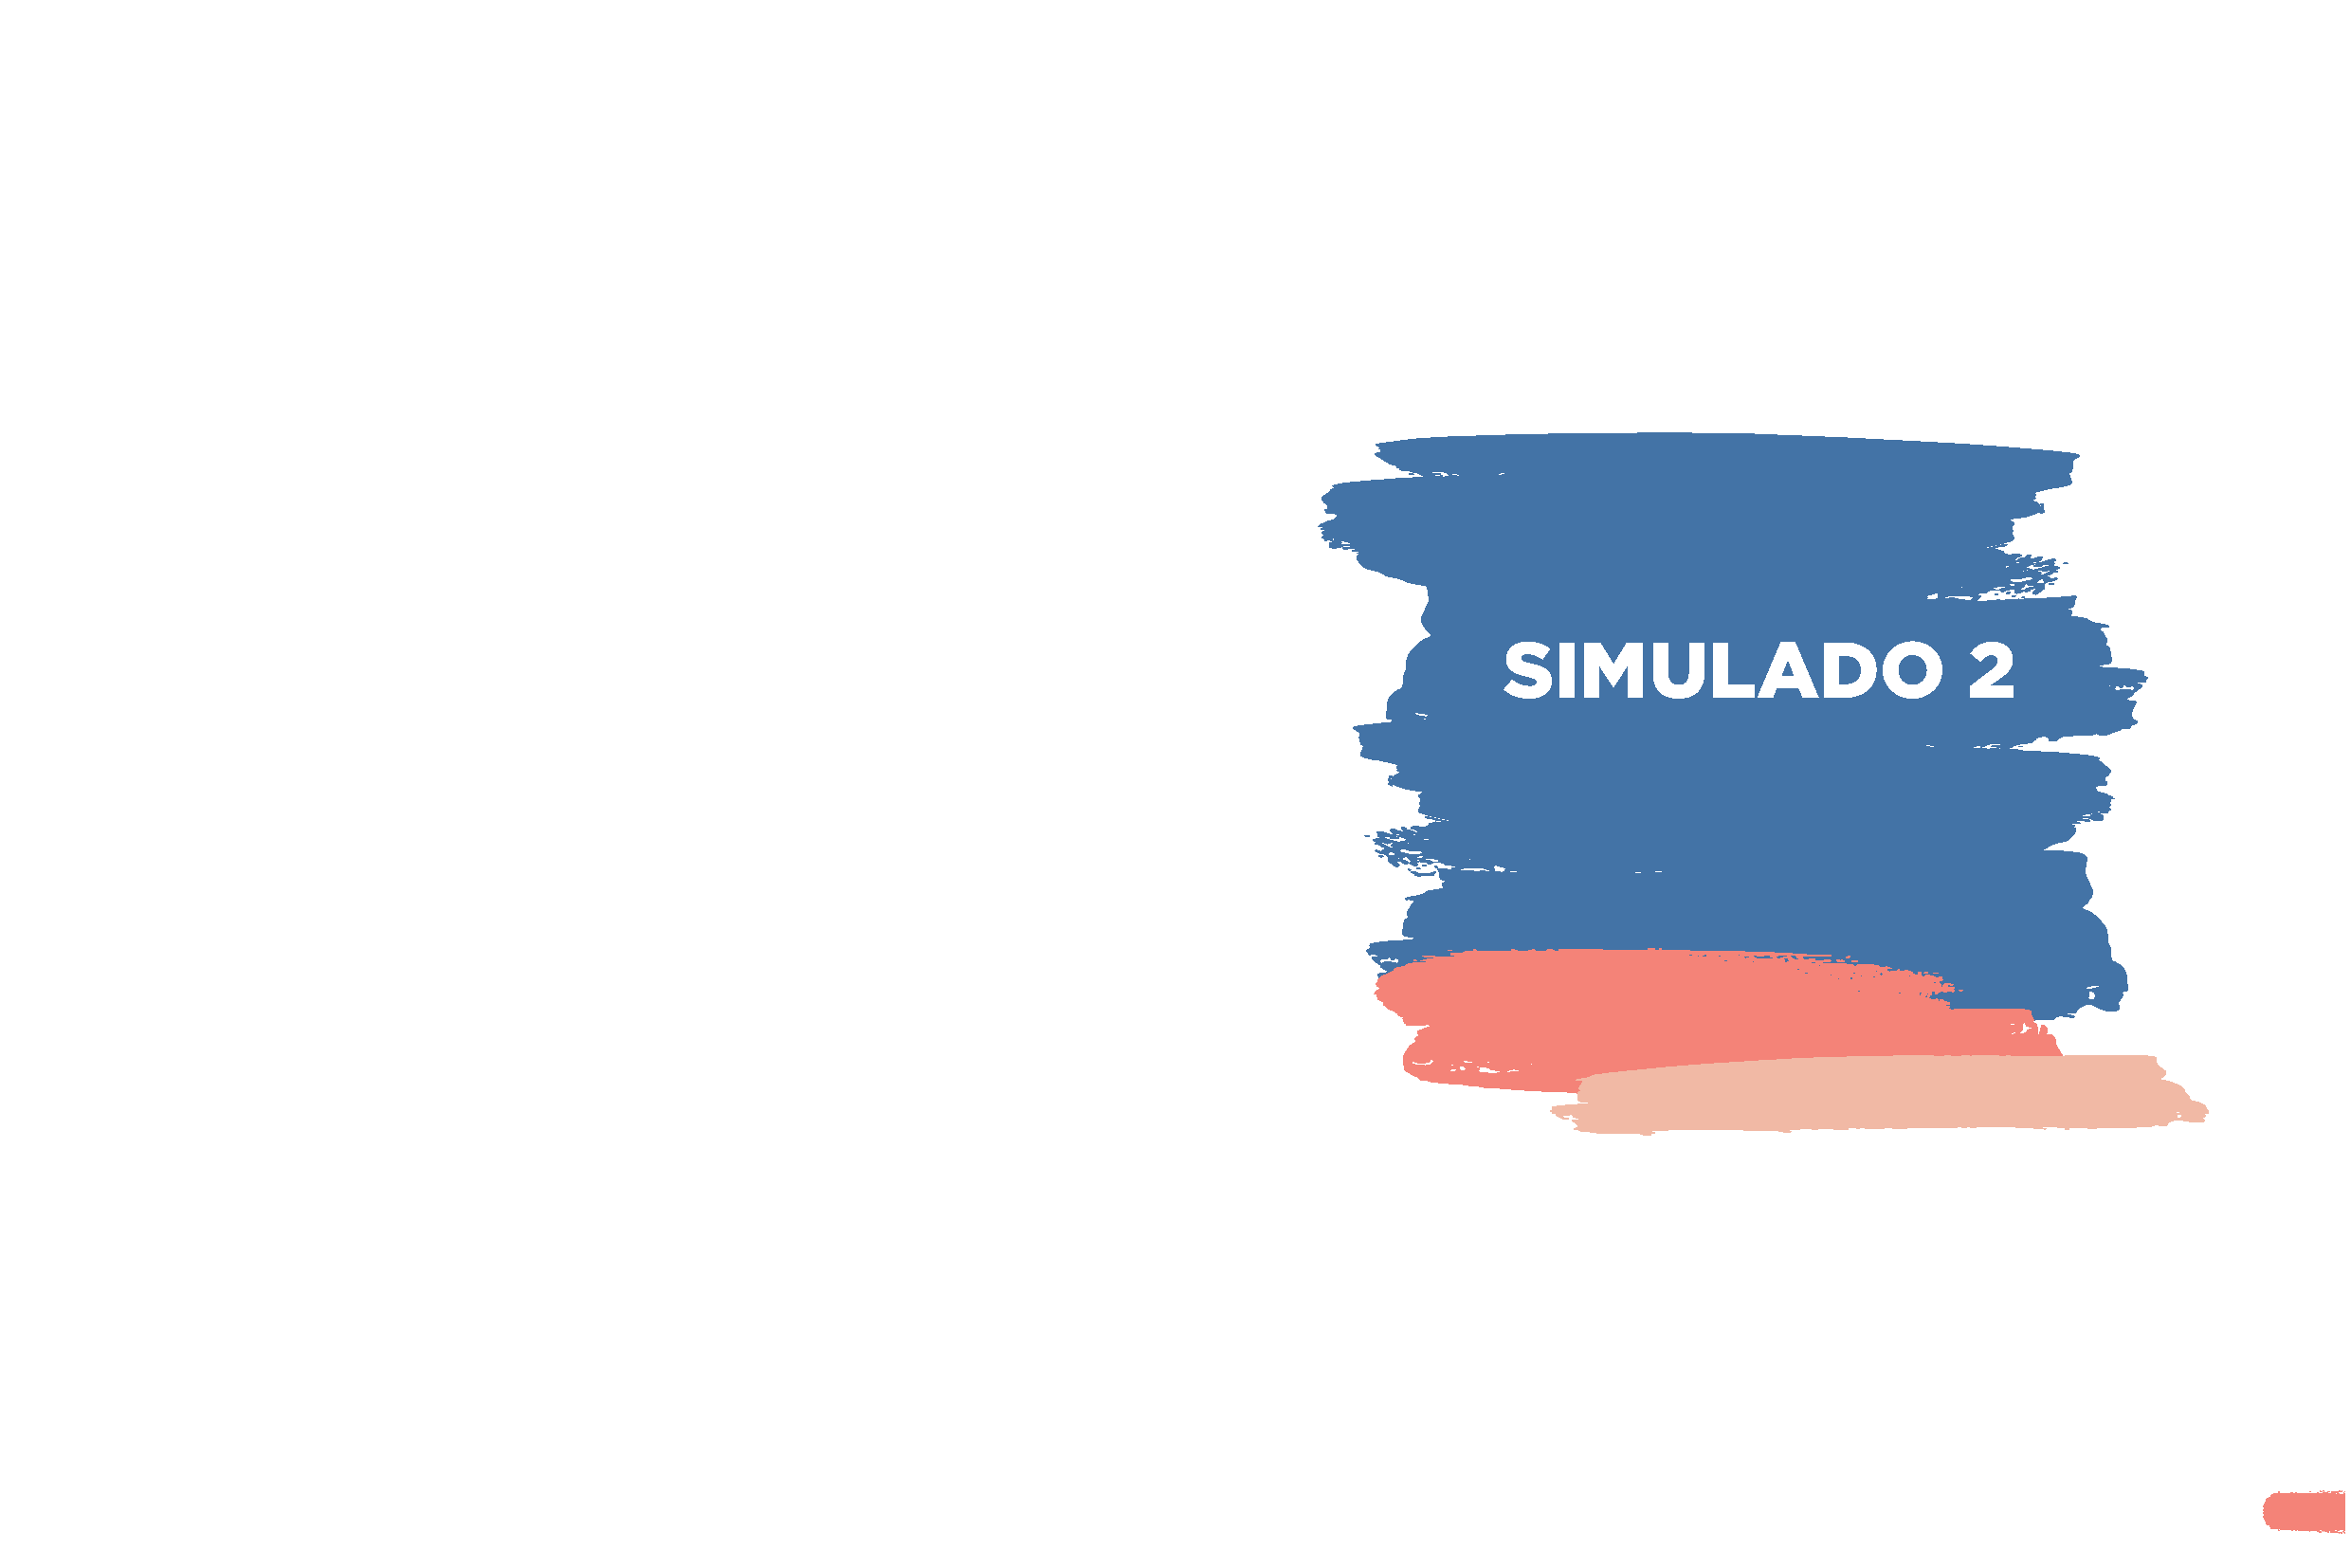
\includegraphics[scale=1]{../watermarks/2simulado5ano.pdf}
\addcontentsline{toc}{chapter}{Simulado 2}
\markboth{Simulado 2}{}

\pagebreak
\num{1} Fabiano tem peças do material dourado de forma que o maior número
que consegue formar é o 724. Sendo assim, a alternativa que traz uma
possibilidade de peças que ele tem do material dourado é:

\begin{escolha}
\item
  6 placas, 4 barras e 6 cubinhos.
\item
  6 placas, 3 barras e 4 cubinhos.
\item
  7 placas, 4 barras e 3 cubinhos.
\item
  7 placas, 2 barras e 4 cubinhos.
\end{escolha}

\num{2} Isabeli quer colocar o número 380 em uma reta numérica igual à representada:

\begin{figure}[htpb!]
\centering
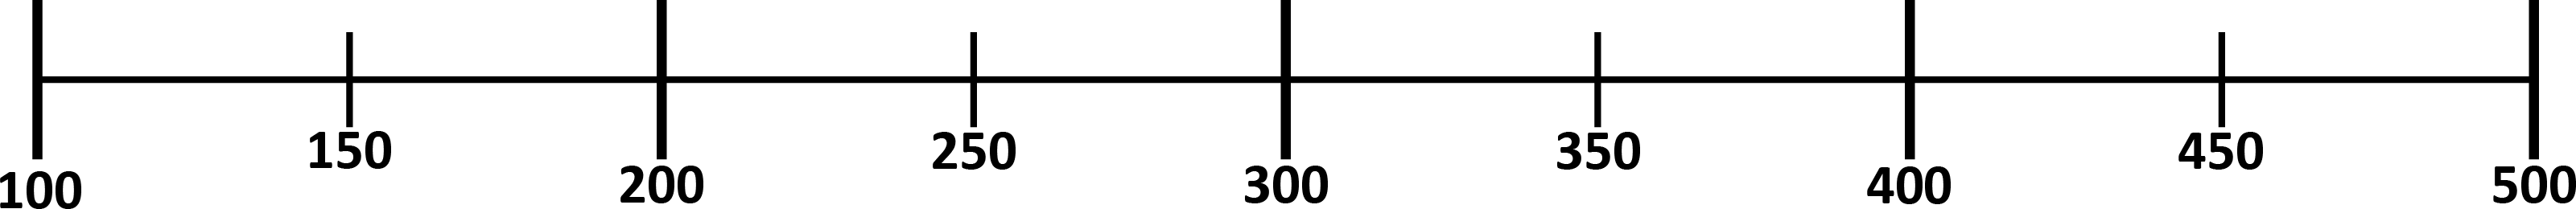
\includegraphics[width=\textwidth]{./media/image102.png}
\end{figure}

Entre quais números que aparecem na reta, Isabeli deverá colocar o número 380?

\begin{multicols}{2}
\begin{escolha}
\item
  Entre 150 e 200.
\item
  Entre 250 e 300.
\item
  Entre 350 e 400.
\item
  Entre 450 e 500.
\end{escolha}
\end{multicols}


\num{3} Gilberto tem as seguintes peças do material dourado:

\begin{figure}[htpb!]
\centering
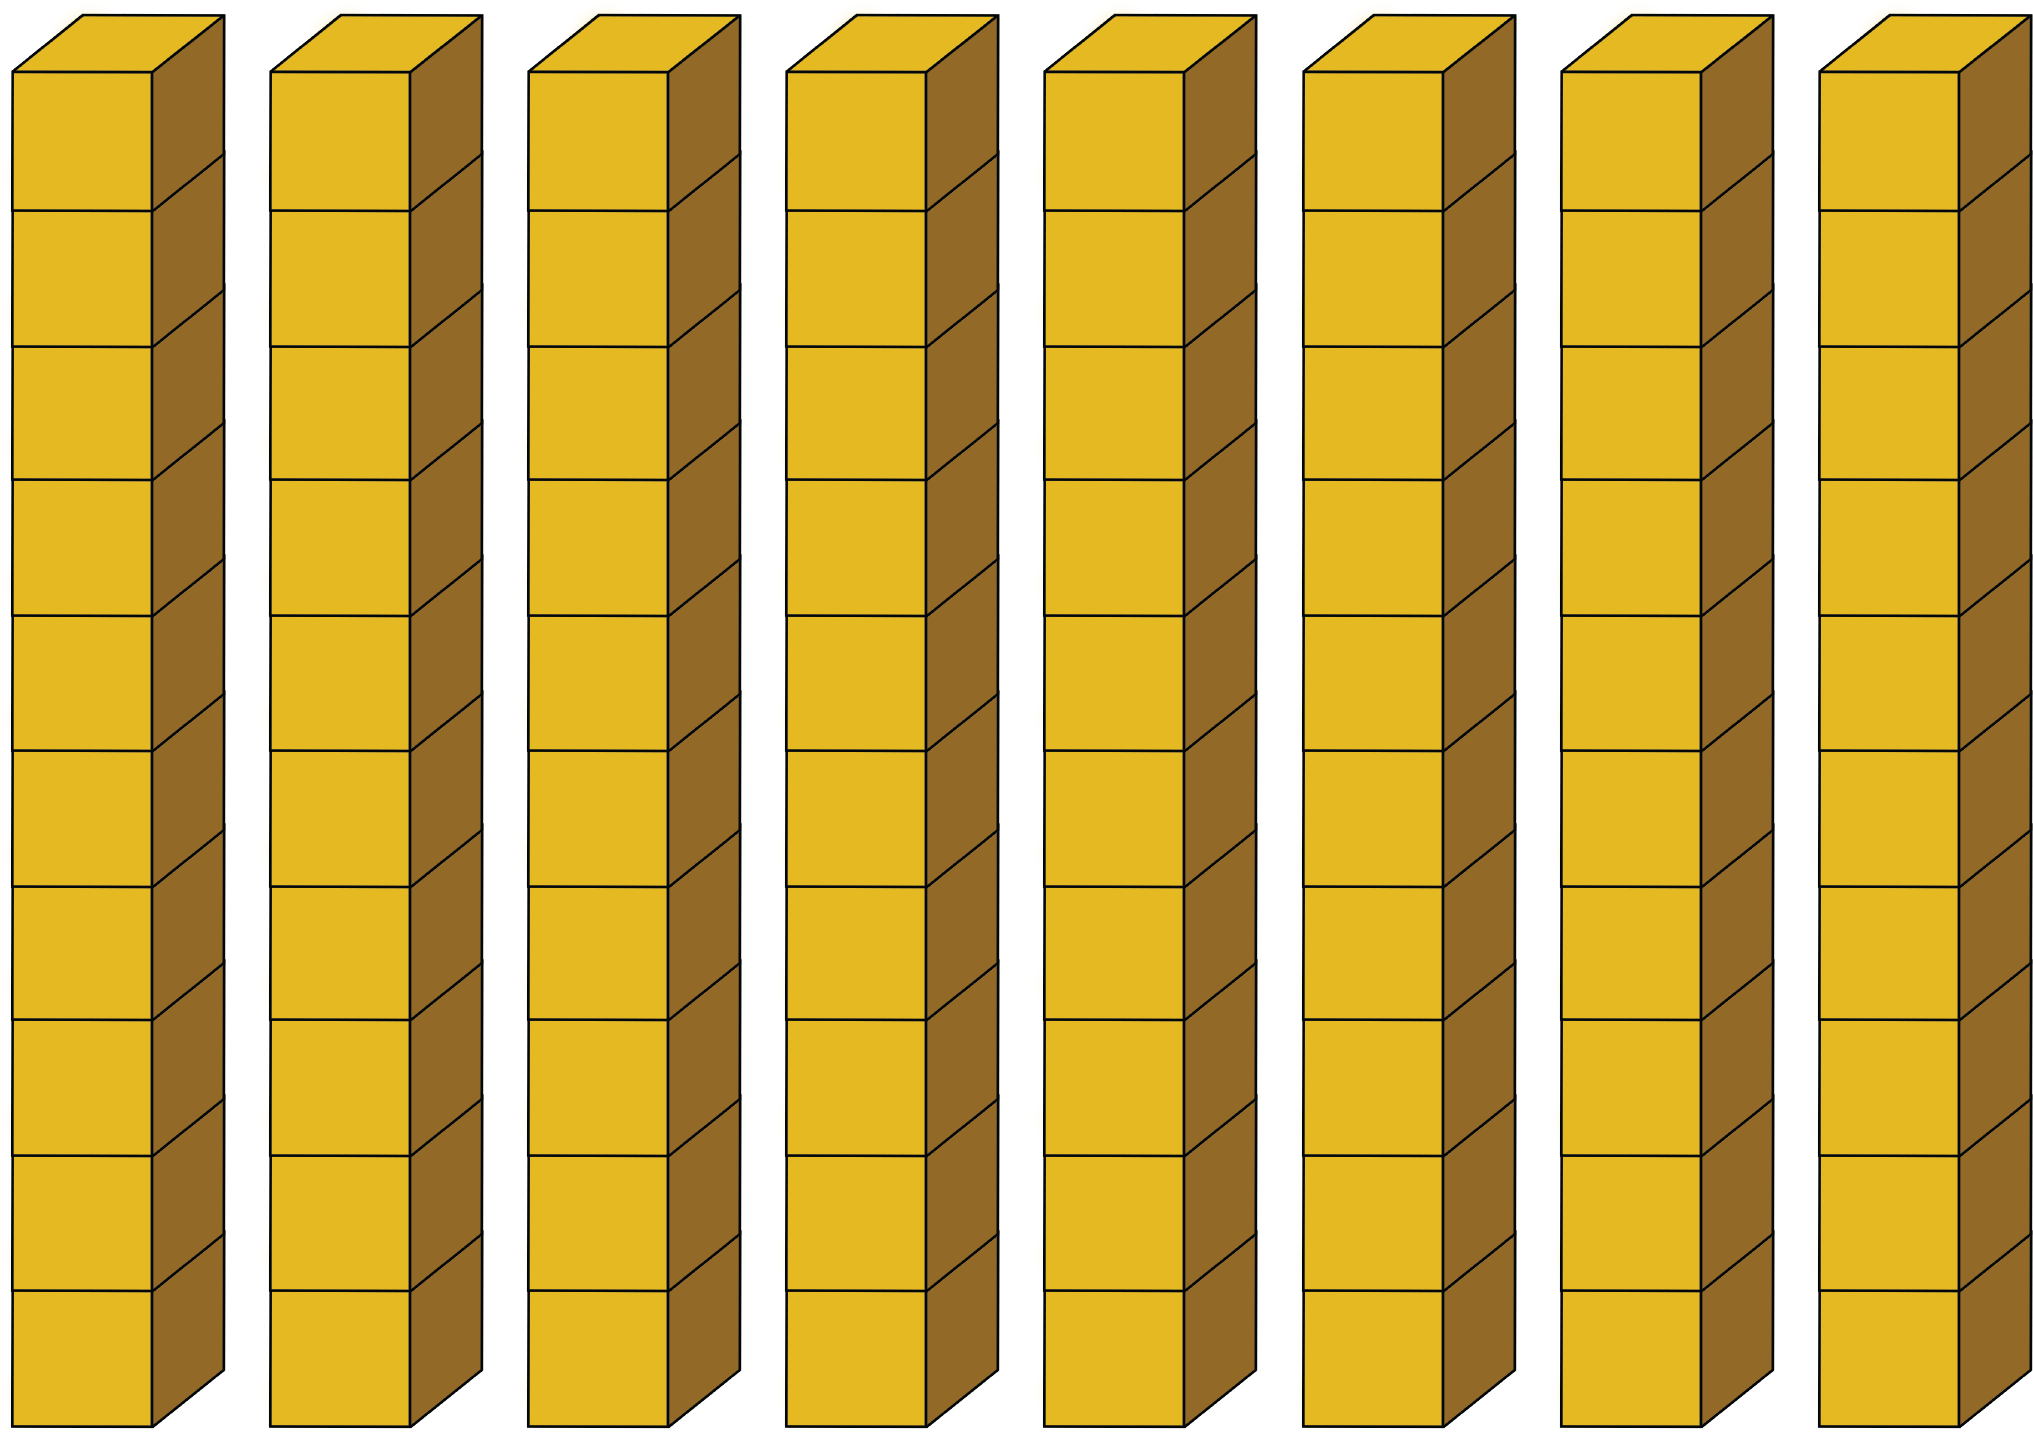
\includegraphics[width=.5\textwidth]{./media/image103.png}
\end{figure}

Quantas barras, no mínimo, ele ainda precisará juntar a essas para conseguir trocar por duas placas?

\begin{escolha}
\item
  3.
\item
  10.
\item
  12.
\item
  20.
\end{escolha}

\num{4} Um lote de 26.104 lápis será embalado em caixas contendo 13 unidades de
lápis em cada. Essas caixas serão distribuídas uma para cada escola
estadual que existe na região em que Lucas mora. Quantas escolas
receberão uma caixa contendo lápis?

\begin{escolha}
\item
  26.
\item
  28.
\item
  208.
\item
  2.008.
\end{escolha}

\num{5} Analisando a sequência, pode-se afirmar que ela segue uma lógica. Qual seria, segundo essa lógica, o próximo número da sequência?

\begin{myquote}
\centering
\textbf{240; 120; 60; 30; ...}
\end{myquote}

\begin{multicols}{2}
\begin{escolha}
\item
  20.
\item
  15.
\item
  10.
\item
  5.
\end{escolha}
\end{multicols}


\num{6} Raquel completará 11 anos daqui a 5 semanas e 2 dias. Quantos dias faltam para ela completar 12 anos?

\begin{multicols}{2}
\begin{escolha}
\item
  37.
\item
  27.
\item
  17.
\item
  7.
\end{escolha}
\end{multicols}

\num{7} Um marceneiro quer medir uma tábua, mas esqueceu-se da sua trena. Dessa forma, resolveu medir com seu palmo, que mede aproximadamente 21 cm.

\begin{figure}[htpb!]
\centering
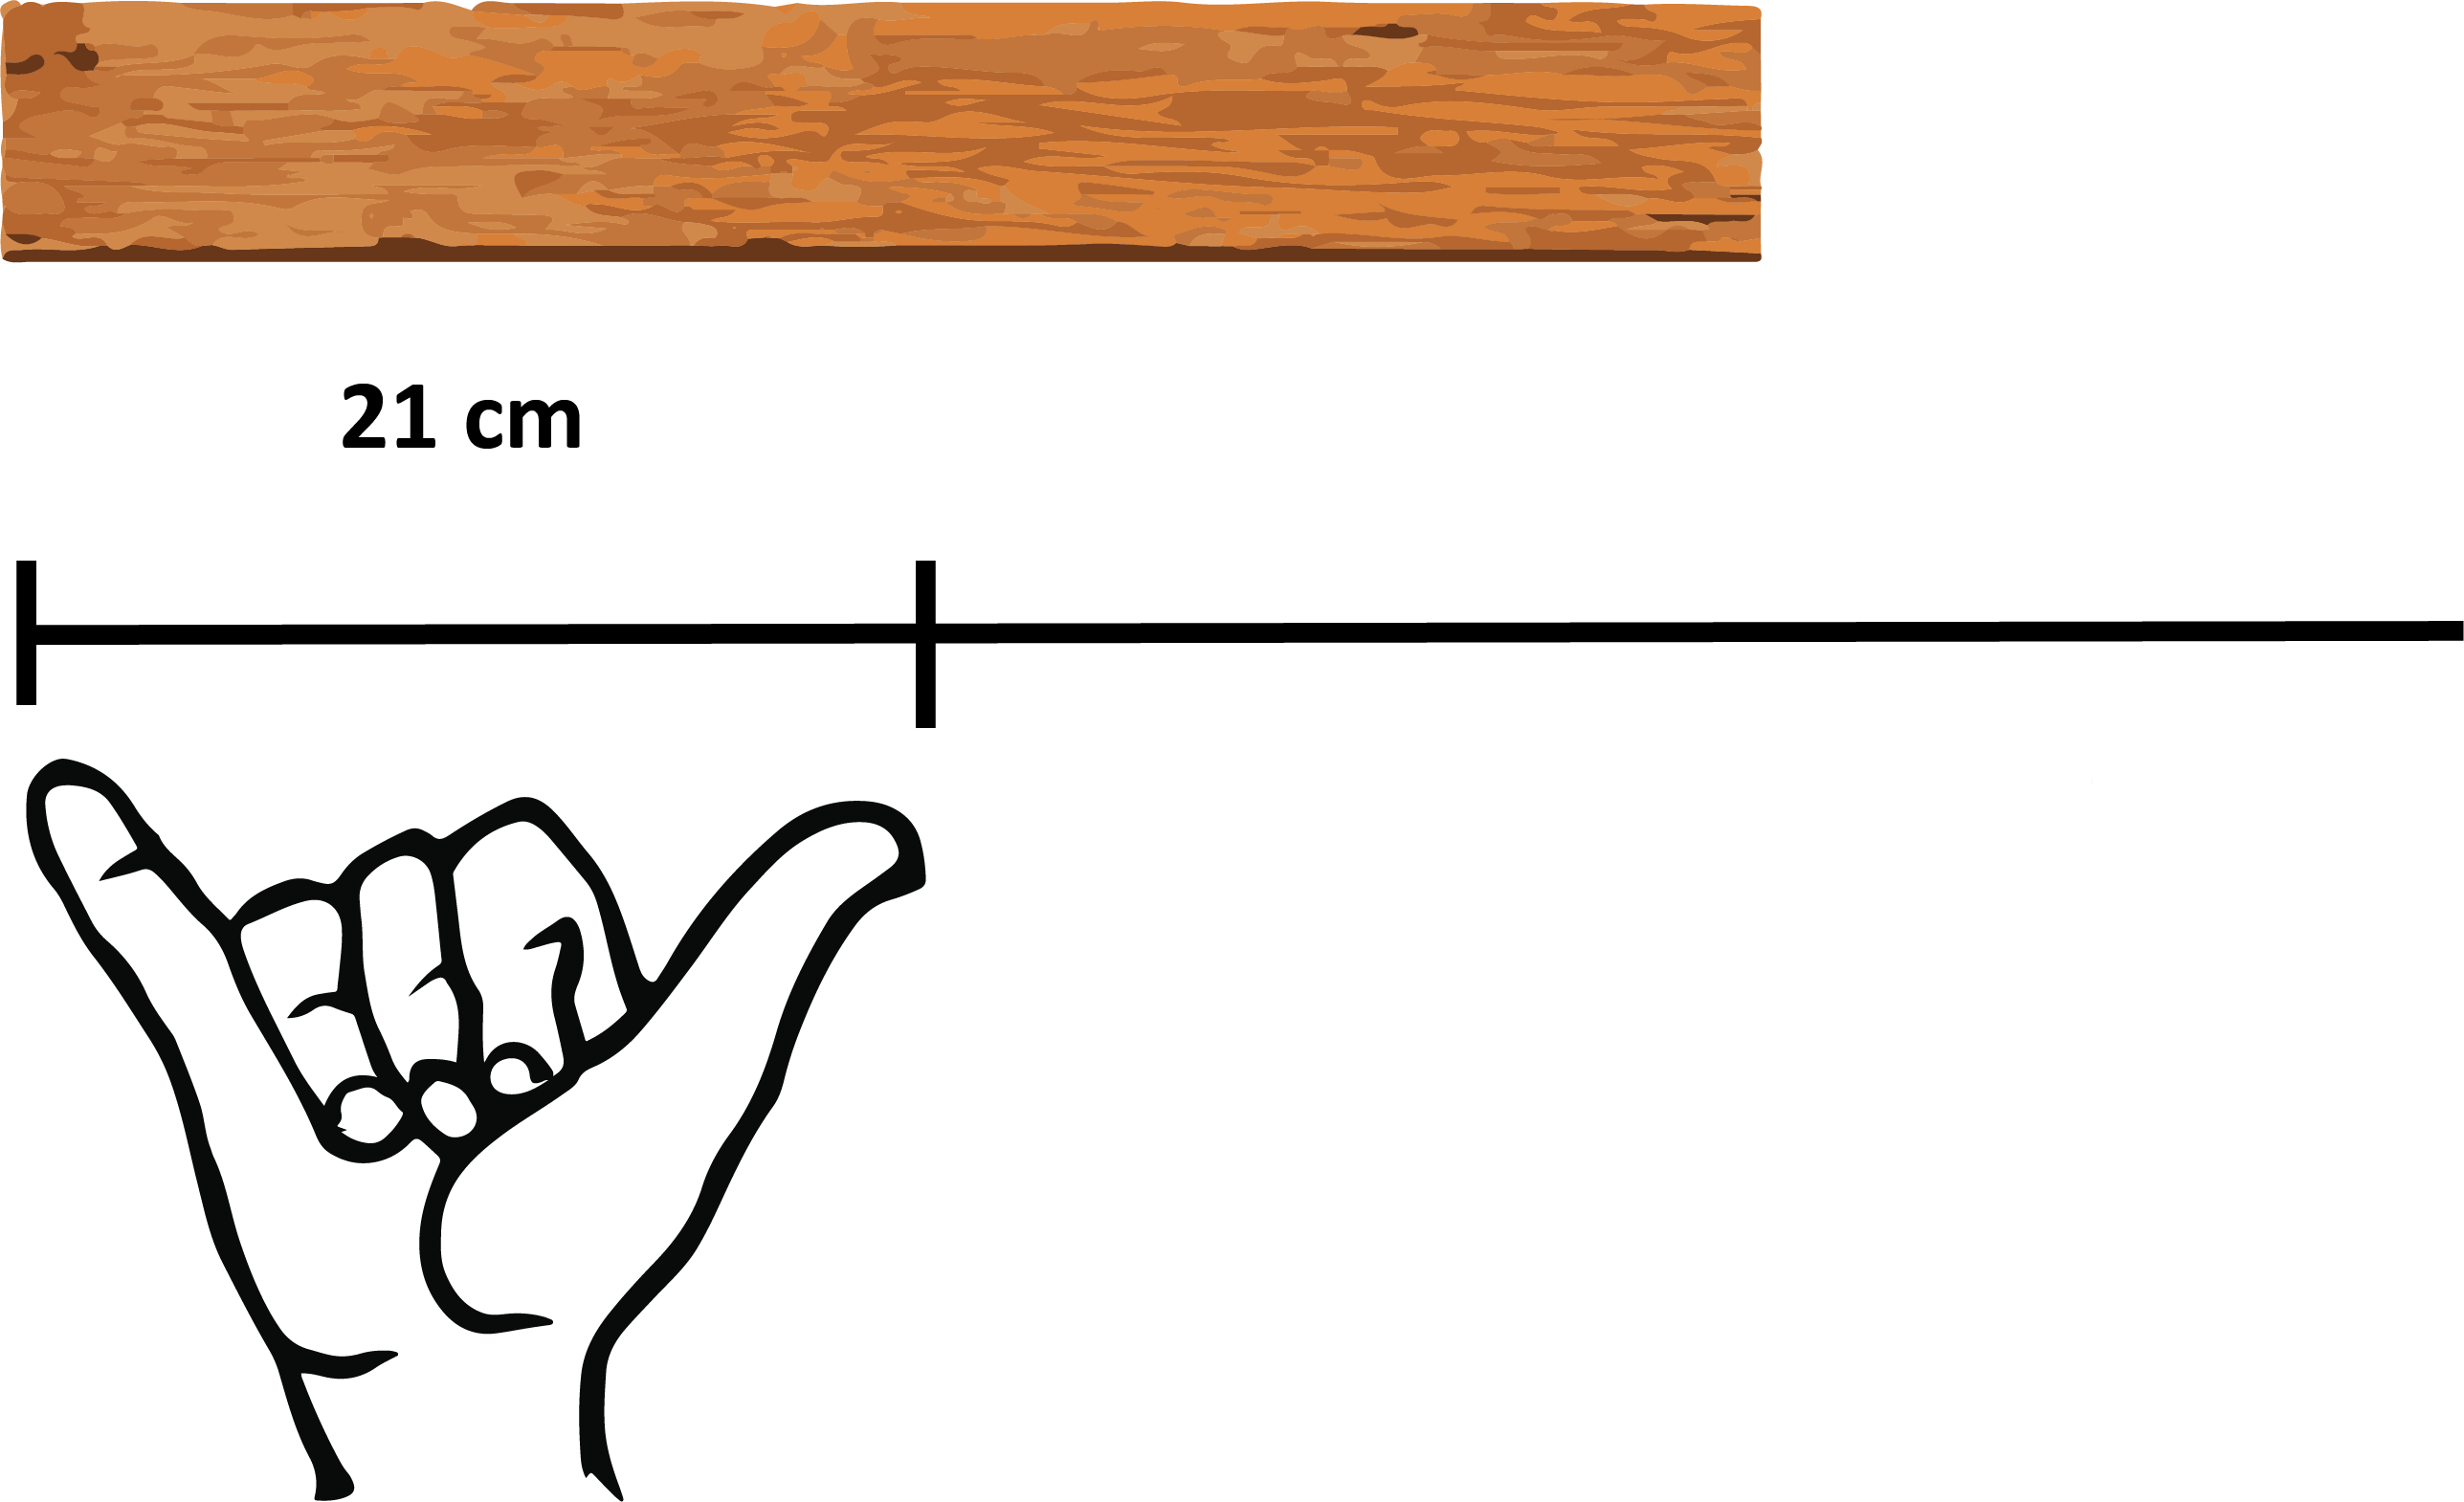
\includegraphics[width=.5\textwidth]{./media/image104.png}
\end{figure}

Sabendo-se que ele chegou à conclusão de que a tábua possui o comprimento de 7 palmos seus, podemos afirmar que a tábua terá uma medida aproximada de

\begin{multicols}{2}
\begin{escolha}
\item
  1,10 m.
\item
  1,30 m.
\item
  1,50 m.
\item
  1,60 m.
\end{escolha}
\end{multicols}

\num{8} Observando um calendário, José queria lembrar-se de qual é o mês que pode ter 28 ou 29 dias. Após pensar um pouquinho, ele chegou à conclusão de que era o mês de

\begin{escolha}
\item
  janeiro.
\item
  fevereiro.
\item
  junho.
\item
  agosto.
\end{escolha}

\pagebreak

\num{9} Maria Luísa resolveu trocar as moedas que ganhou de seu avô por notas de
2 reais com o seu primo, Francisco. No cofre da menina havia 12 moedas de 50
centavos e 8 moedas de 25 centavos. Quantas notas de 2 reais ela recebeu
de seu primo nessa troca?

\begin{escolha}
\item
  4.
\item
  6.
\item
  8.
\item
  20.
\end{escolha}

\num{10} Isac estava conferindo o estoque de mercadorias de sua loja e percebeu que, inicialmente, ele tinha 200 peças; depois vendeu 2 caixas com peças para Carlos. Em cada uma das caixas havia um pacote com 5 unidades de peças e dois pacotes com 7 peças.

Para saber a quantidade de peças que restavam no estoque, Isac fez a seguinte anotação:

\begin{myquote}
\centering
\textbf{200 -- 2 x (1 x 5 + 2 x 7)}
\end{myquote}

O resultado dessa expressão era exatamente igual à quantidade de peças que restavam em seu estoque após a venda para Carlos. Qual é a quantidade de peças que Isac possui agora em seu estoque?

\begin{multicols}{2}
\begin{escolha}
\item
  72.
\item
  94.
\item
  126.
\item
  162.
\end{escolha}
\end{multicols}

\pagebreak

\num{11} O gráfico mostra a quantidade de bolas que uma loja de artigos esportivos vendeu durante os meses que antecederam uma edição da copa do mundo de futebol.

\begin{figure}[htpb!]
\centering
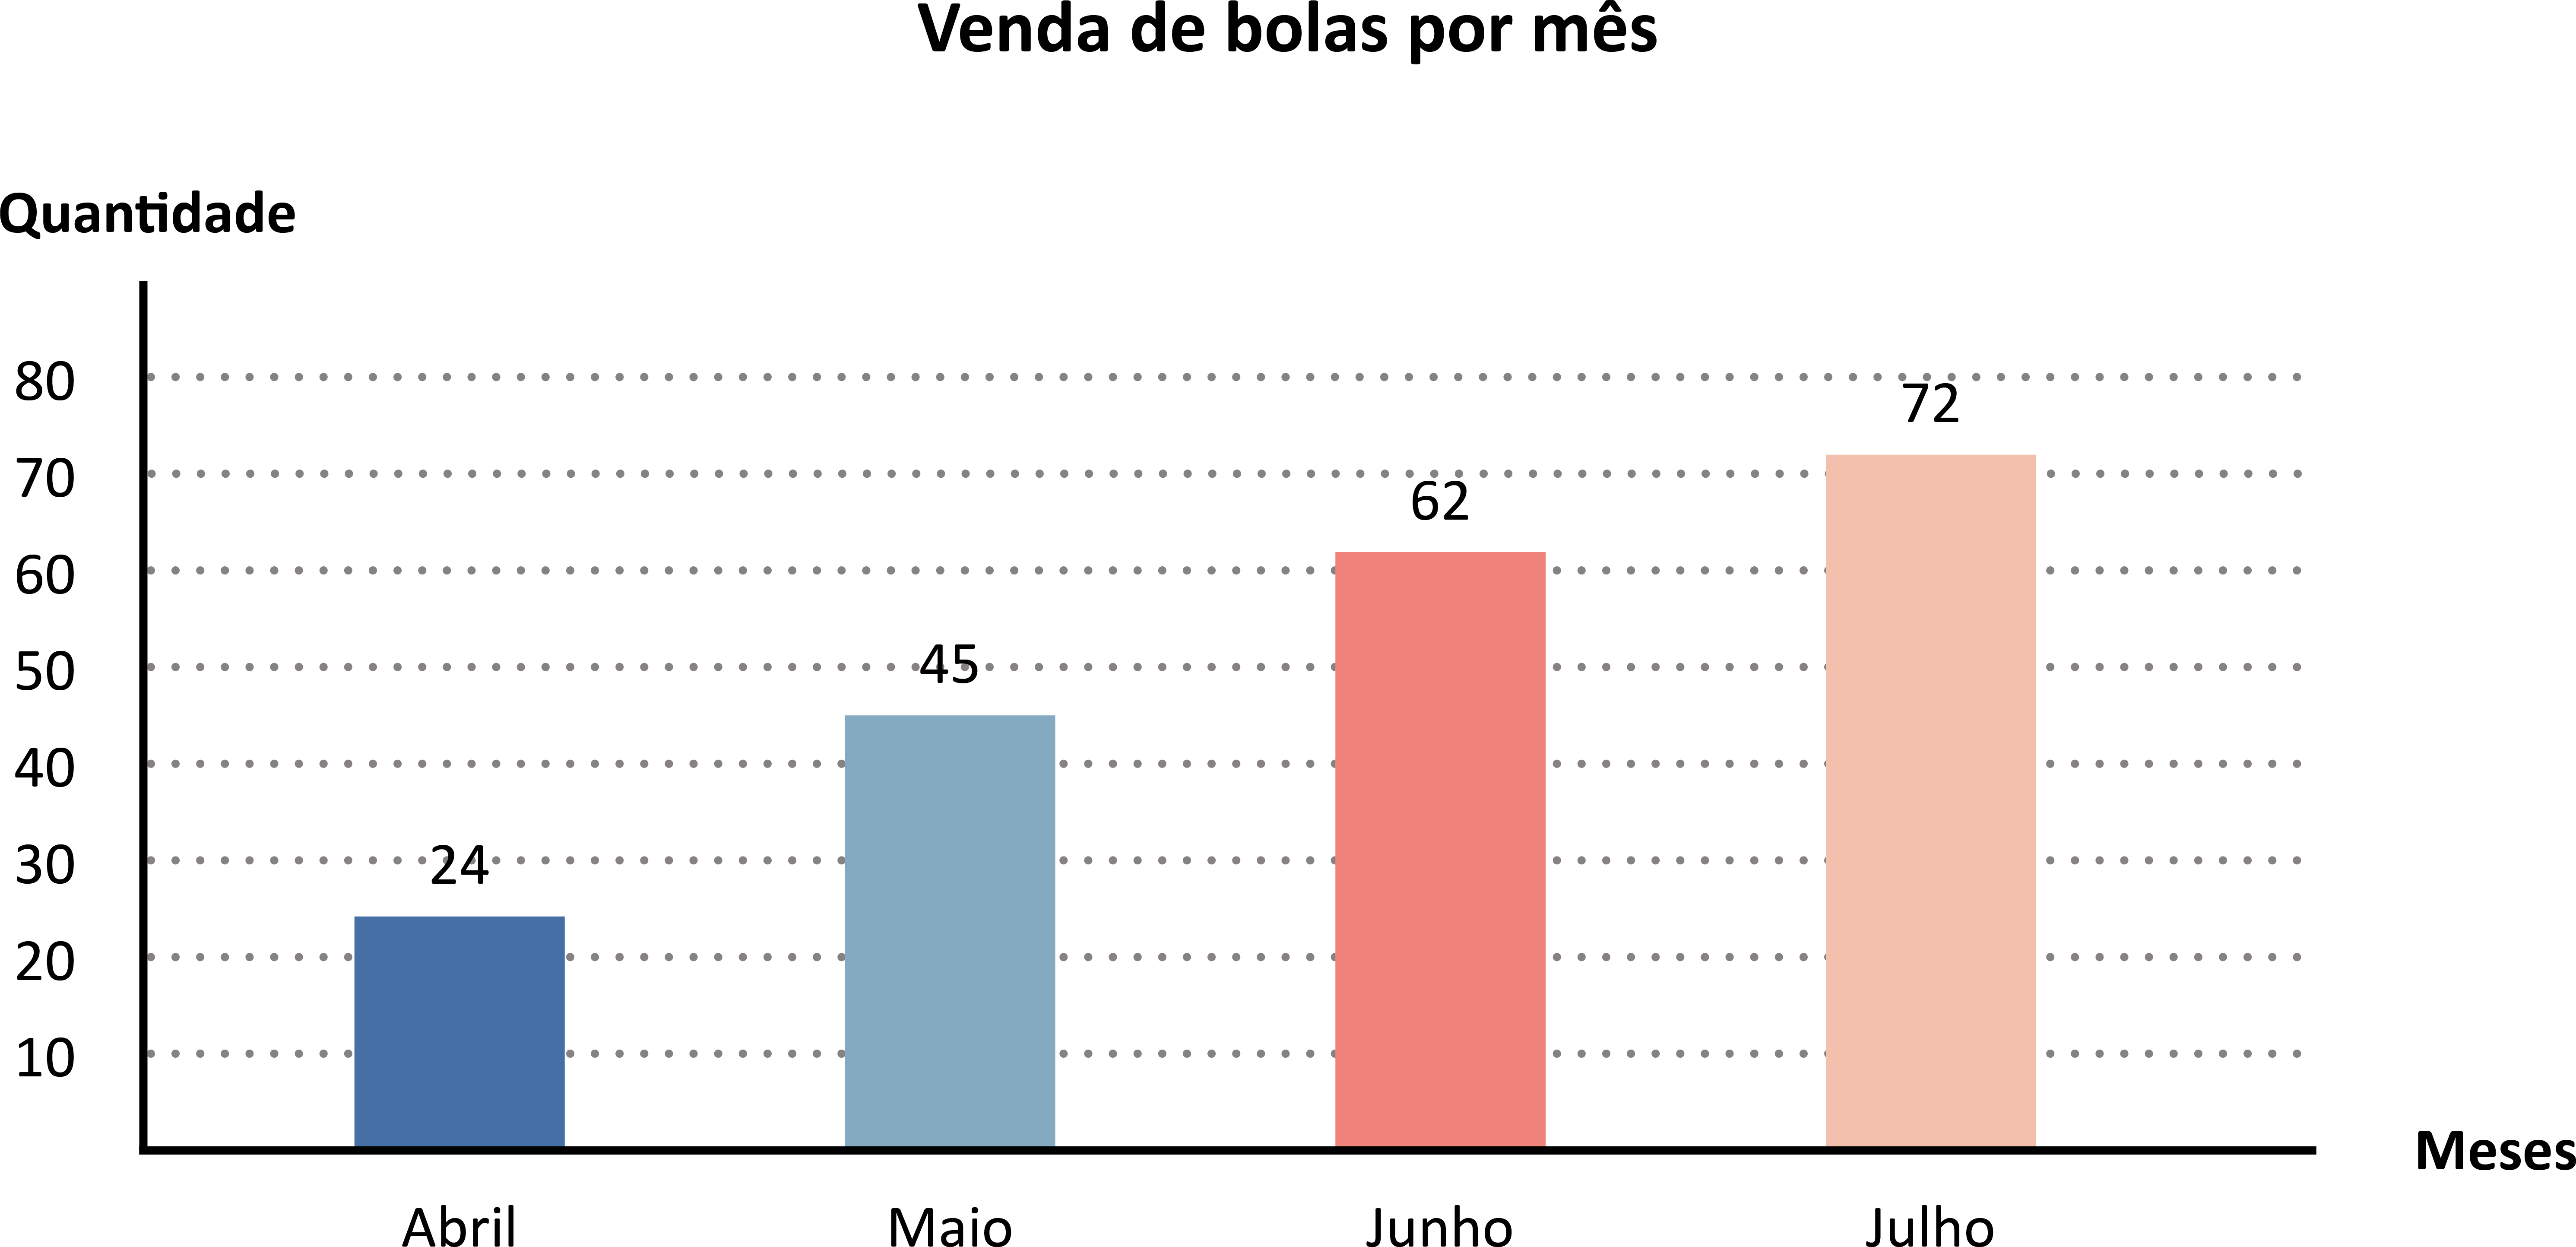
\includegraphics[width=\textwidth]{./media/image105.png}
\end{figure}

Analise o gráfico e responda: em qual mês a quantidade de bolas vendidas foi exatamente o triplo daquela vendida em outro mês?

%\begin{multicols}{2}
\begin{escolha}
\item
  Abril.
\item
  Maio.
\item
  Junho.
\item
  Julho.
\end{escolha}
%\end{multicols}

\pagebreak

\num{12} A biblioteca municipal de uma cidade do interior do Ceará fez uma pesquisa sobre a quantidade de livros retirados pelas pessoas em determinados meses. Veja o resultado:

\begin{figure}[htpb!]
\centering
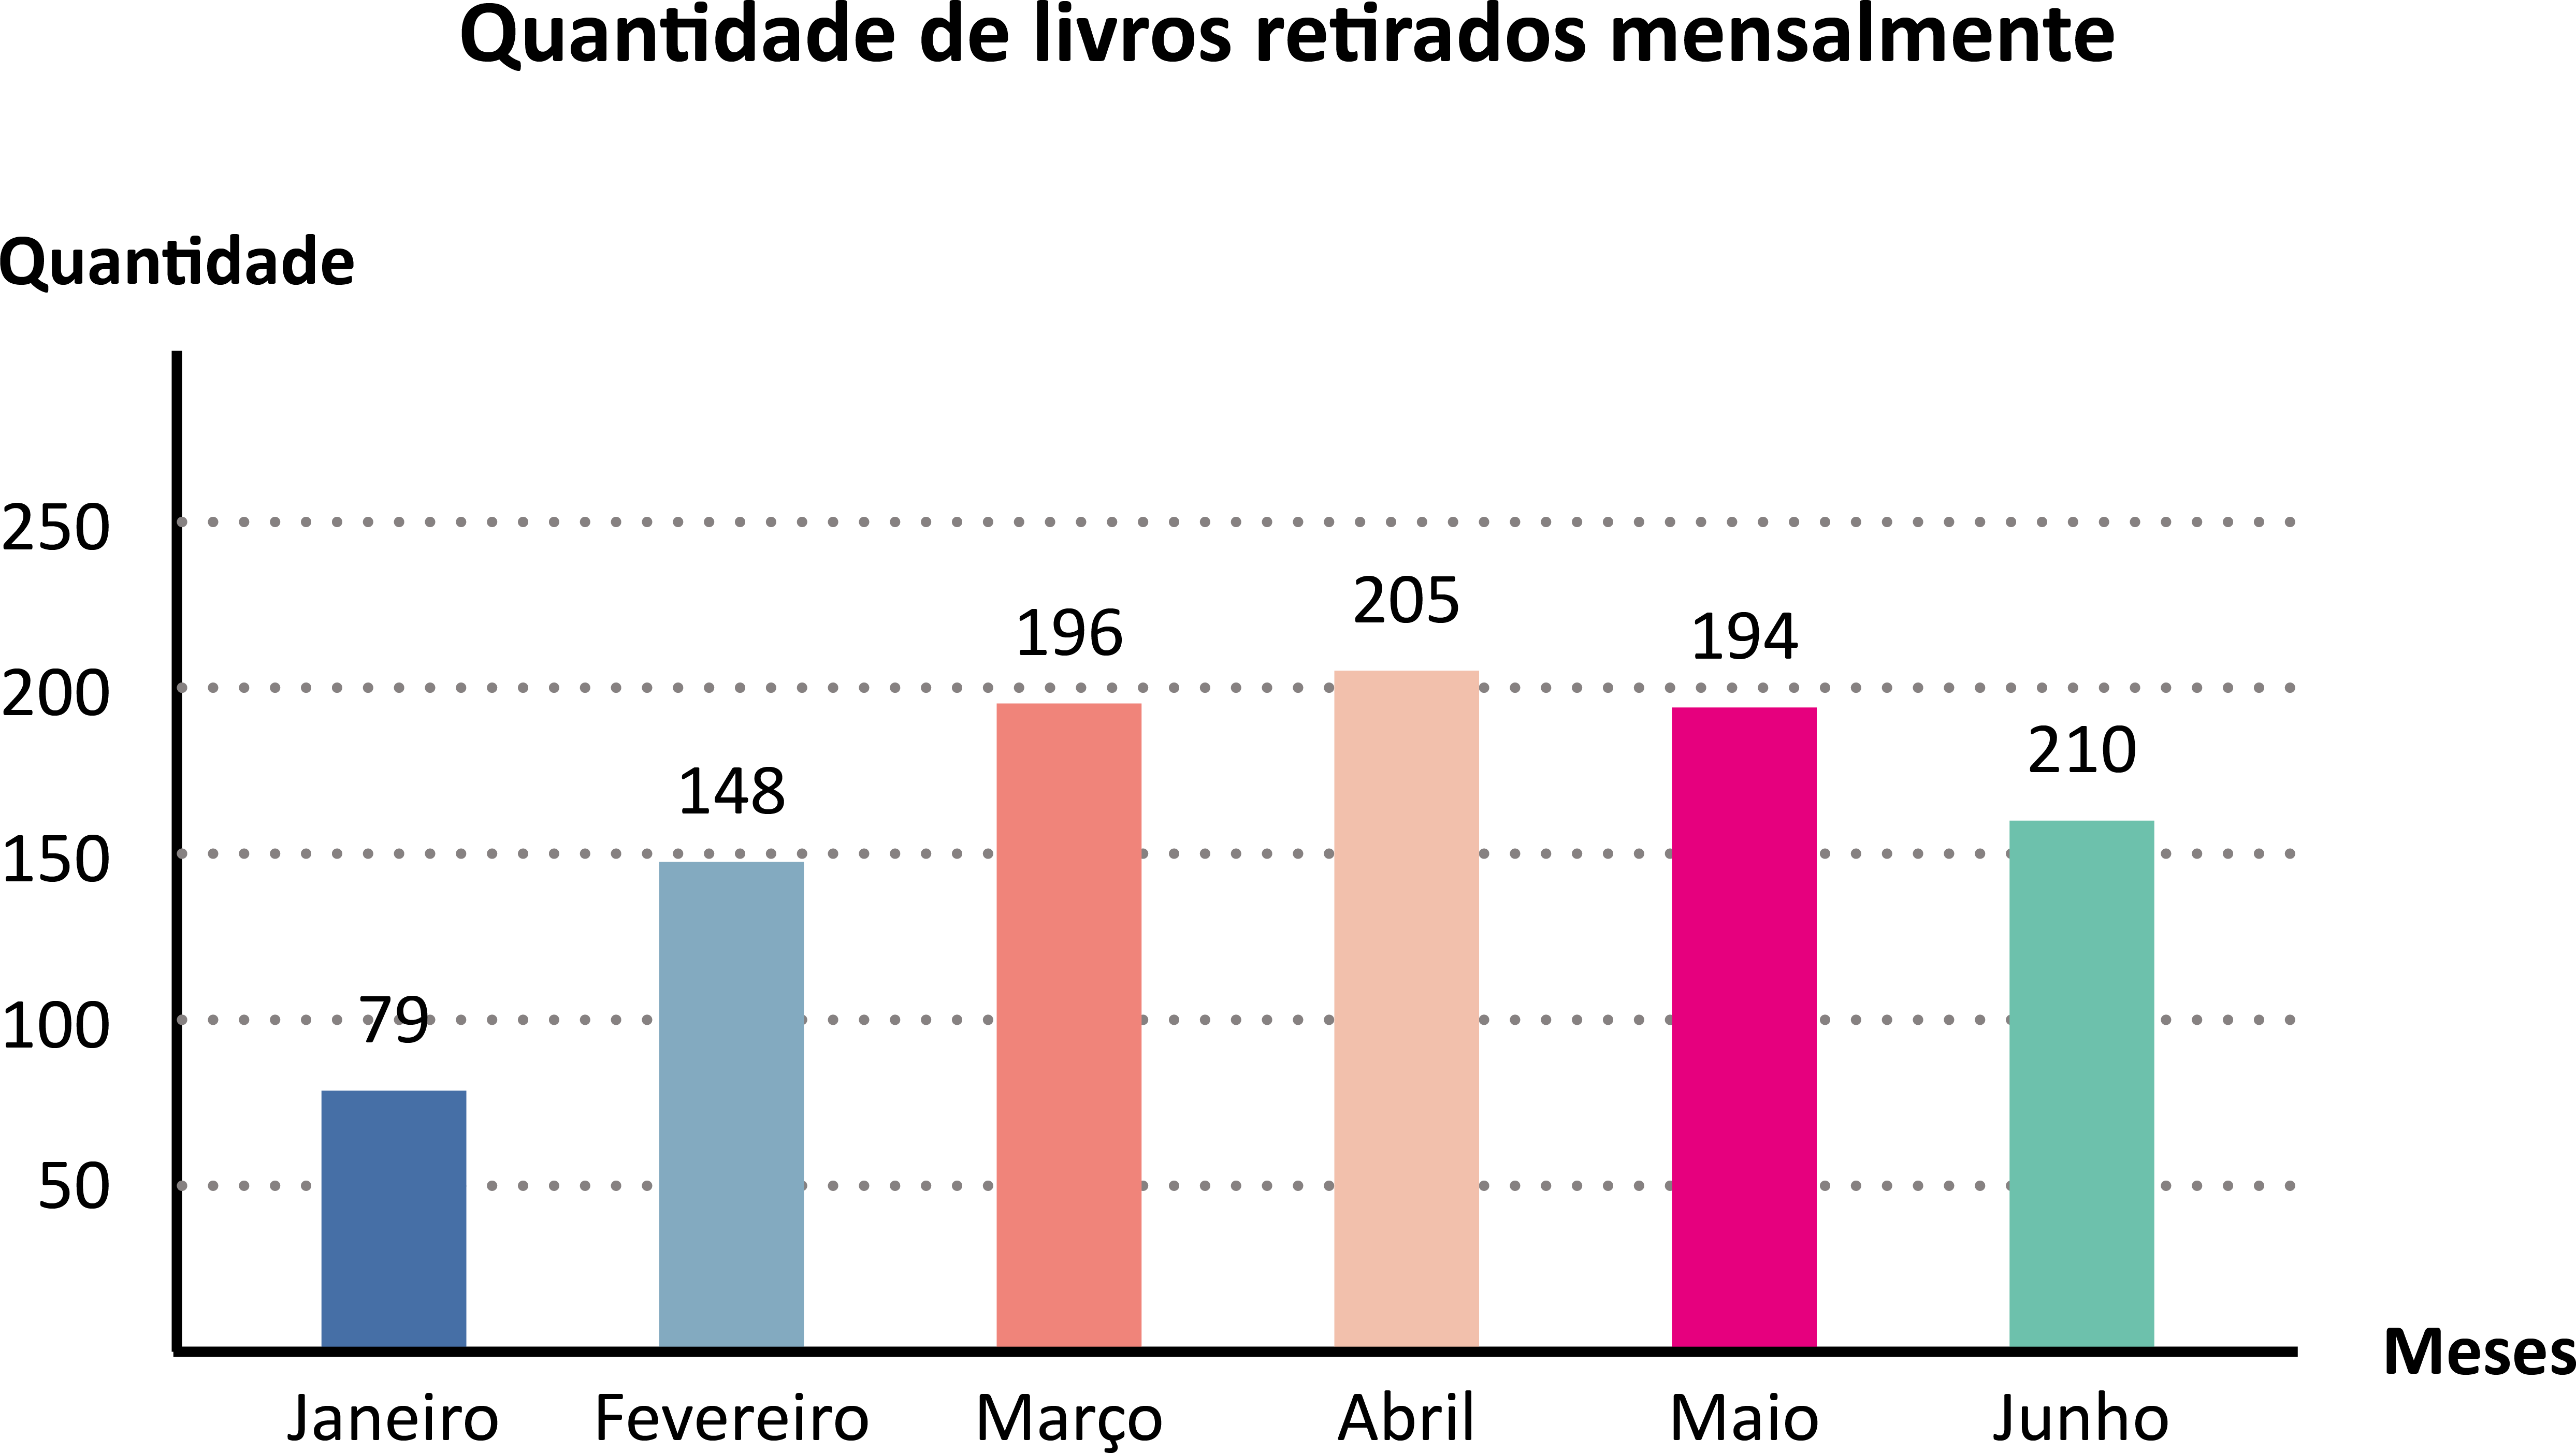
\includegraphics[width=\textwidth]{./media/image106.png}
\end{figure}

Pela análise dos dados, é possivel concluir que

\begin{escolha}
\item
  A quantidade de livros foi crescente mês a mês, de forma linear.
\item
  A quantidade de livros foi decrescente mês a mês, de forma linear.
\item
  Em todos os meses, a quantidade de livros retirados foi praticamente a mesma.
\item
  Com exceção de maio, em todos os demais meses houve aumento crescente nos números.
\end{escolha}
%NOTE: A informação gráfica não corresponde à informação do mês de julho. Pedir correção se for o caso. Checar imagem final.

\pagebreak

\num{13} Maria é especialista em fazer um café delicioso. Segundo a receita que ela segue, utiliza-se uma colher de sopa de pó de café para cada 250 mL de água. Se você, utilizando a receita de Maria, pretende utilizar 750 mL de água, quantas colheres de sopa de pó de café deverá utilizar?

%\begin{multicols}{2}
\begin{escolha}
\item
  2.
\item
  3.
\item
  4.
\item
  5.
\end{escolha}
%\end{multicols}

\num{14} Gabriel foi a um estádio de futebol assistir a um jogo ao vivo pela primeira vez. Os ingressos eram numerados, mas, chegando próximo ao seu
lugar, percebeu que sua cadeira estava sem o número de identificação.

\begin{figure}[htpb!]
\centering
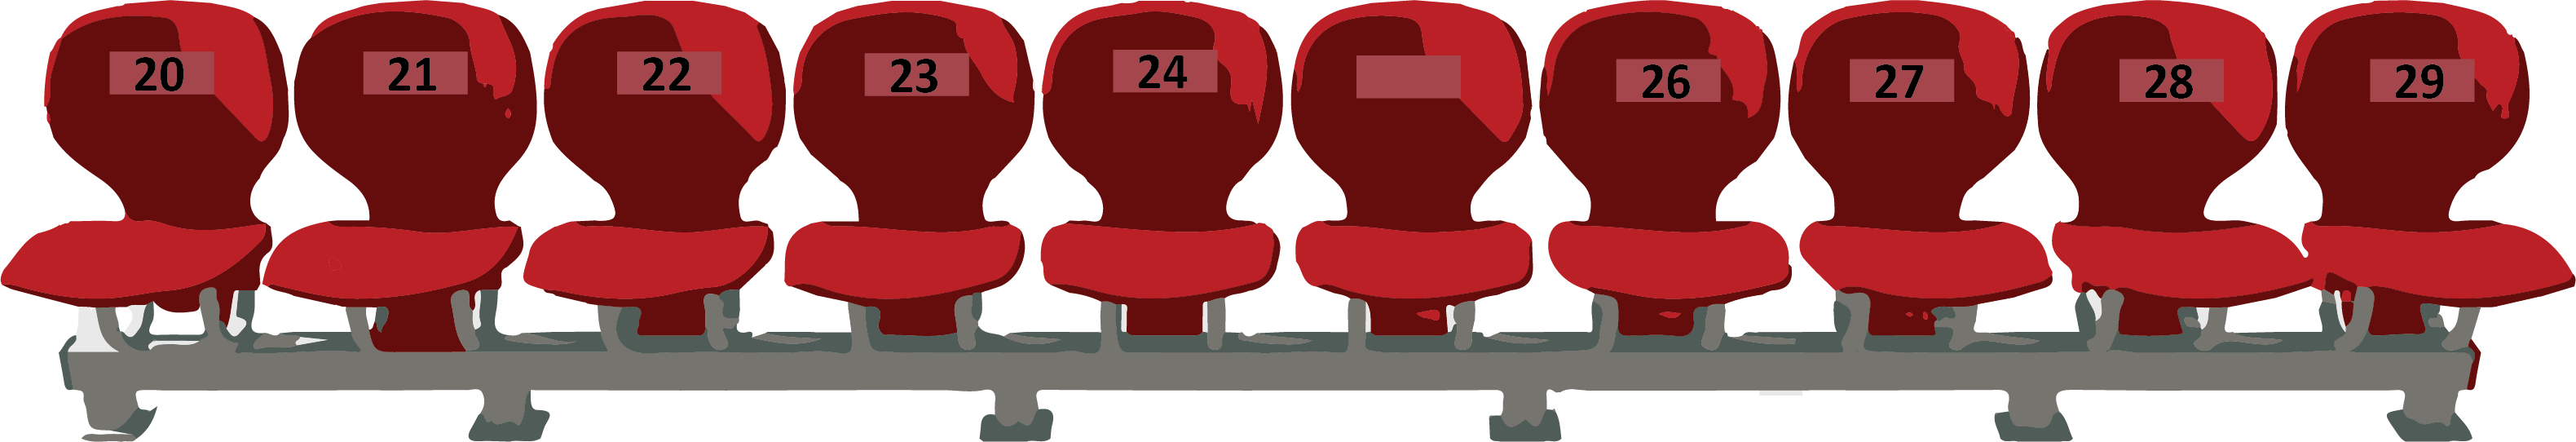
\includegraphics[width=\textwidth]{./media/image107.png}
\end{figure}

Ele parou alguns instantes, relembrando de suas aulas de matemática e concluiu que aquela cadeira sem número era realmente a cadeira que deveria estar com o número impresso em seu ingresso. Qual o número que
deveria estar fixado na cadeira que está sem a placa?
%\begin{multicols}{2}

\begin{escolha}
\item
  30.
\item
  19.
\item
  35.
\item
  25.
\end{escolha}
%\end{multicols}

\pagebreak
\num{15} Dois aplicativos exigem uma senha numérica para serem acessados. Breno criou a senha 6081 para o primeiro e para o segundo utilizou como senha o sucessor do sucessor do número escolhido para a primeira senha. Qual a senha utilizada por Breno para o segundo aplicativo?

%\begin{multicols}{2}
\begin{escolha}
\item
  6.079.
\item
  6.080.
\item
  6.082.
\item
  6.083.
\end{escolha}
%\end{multicols}

\pagebreak

\vspace*{-3.4cm}
%\hspace*{-3.7cm}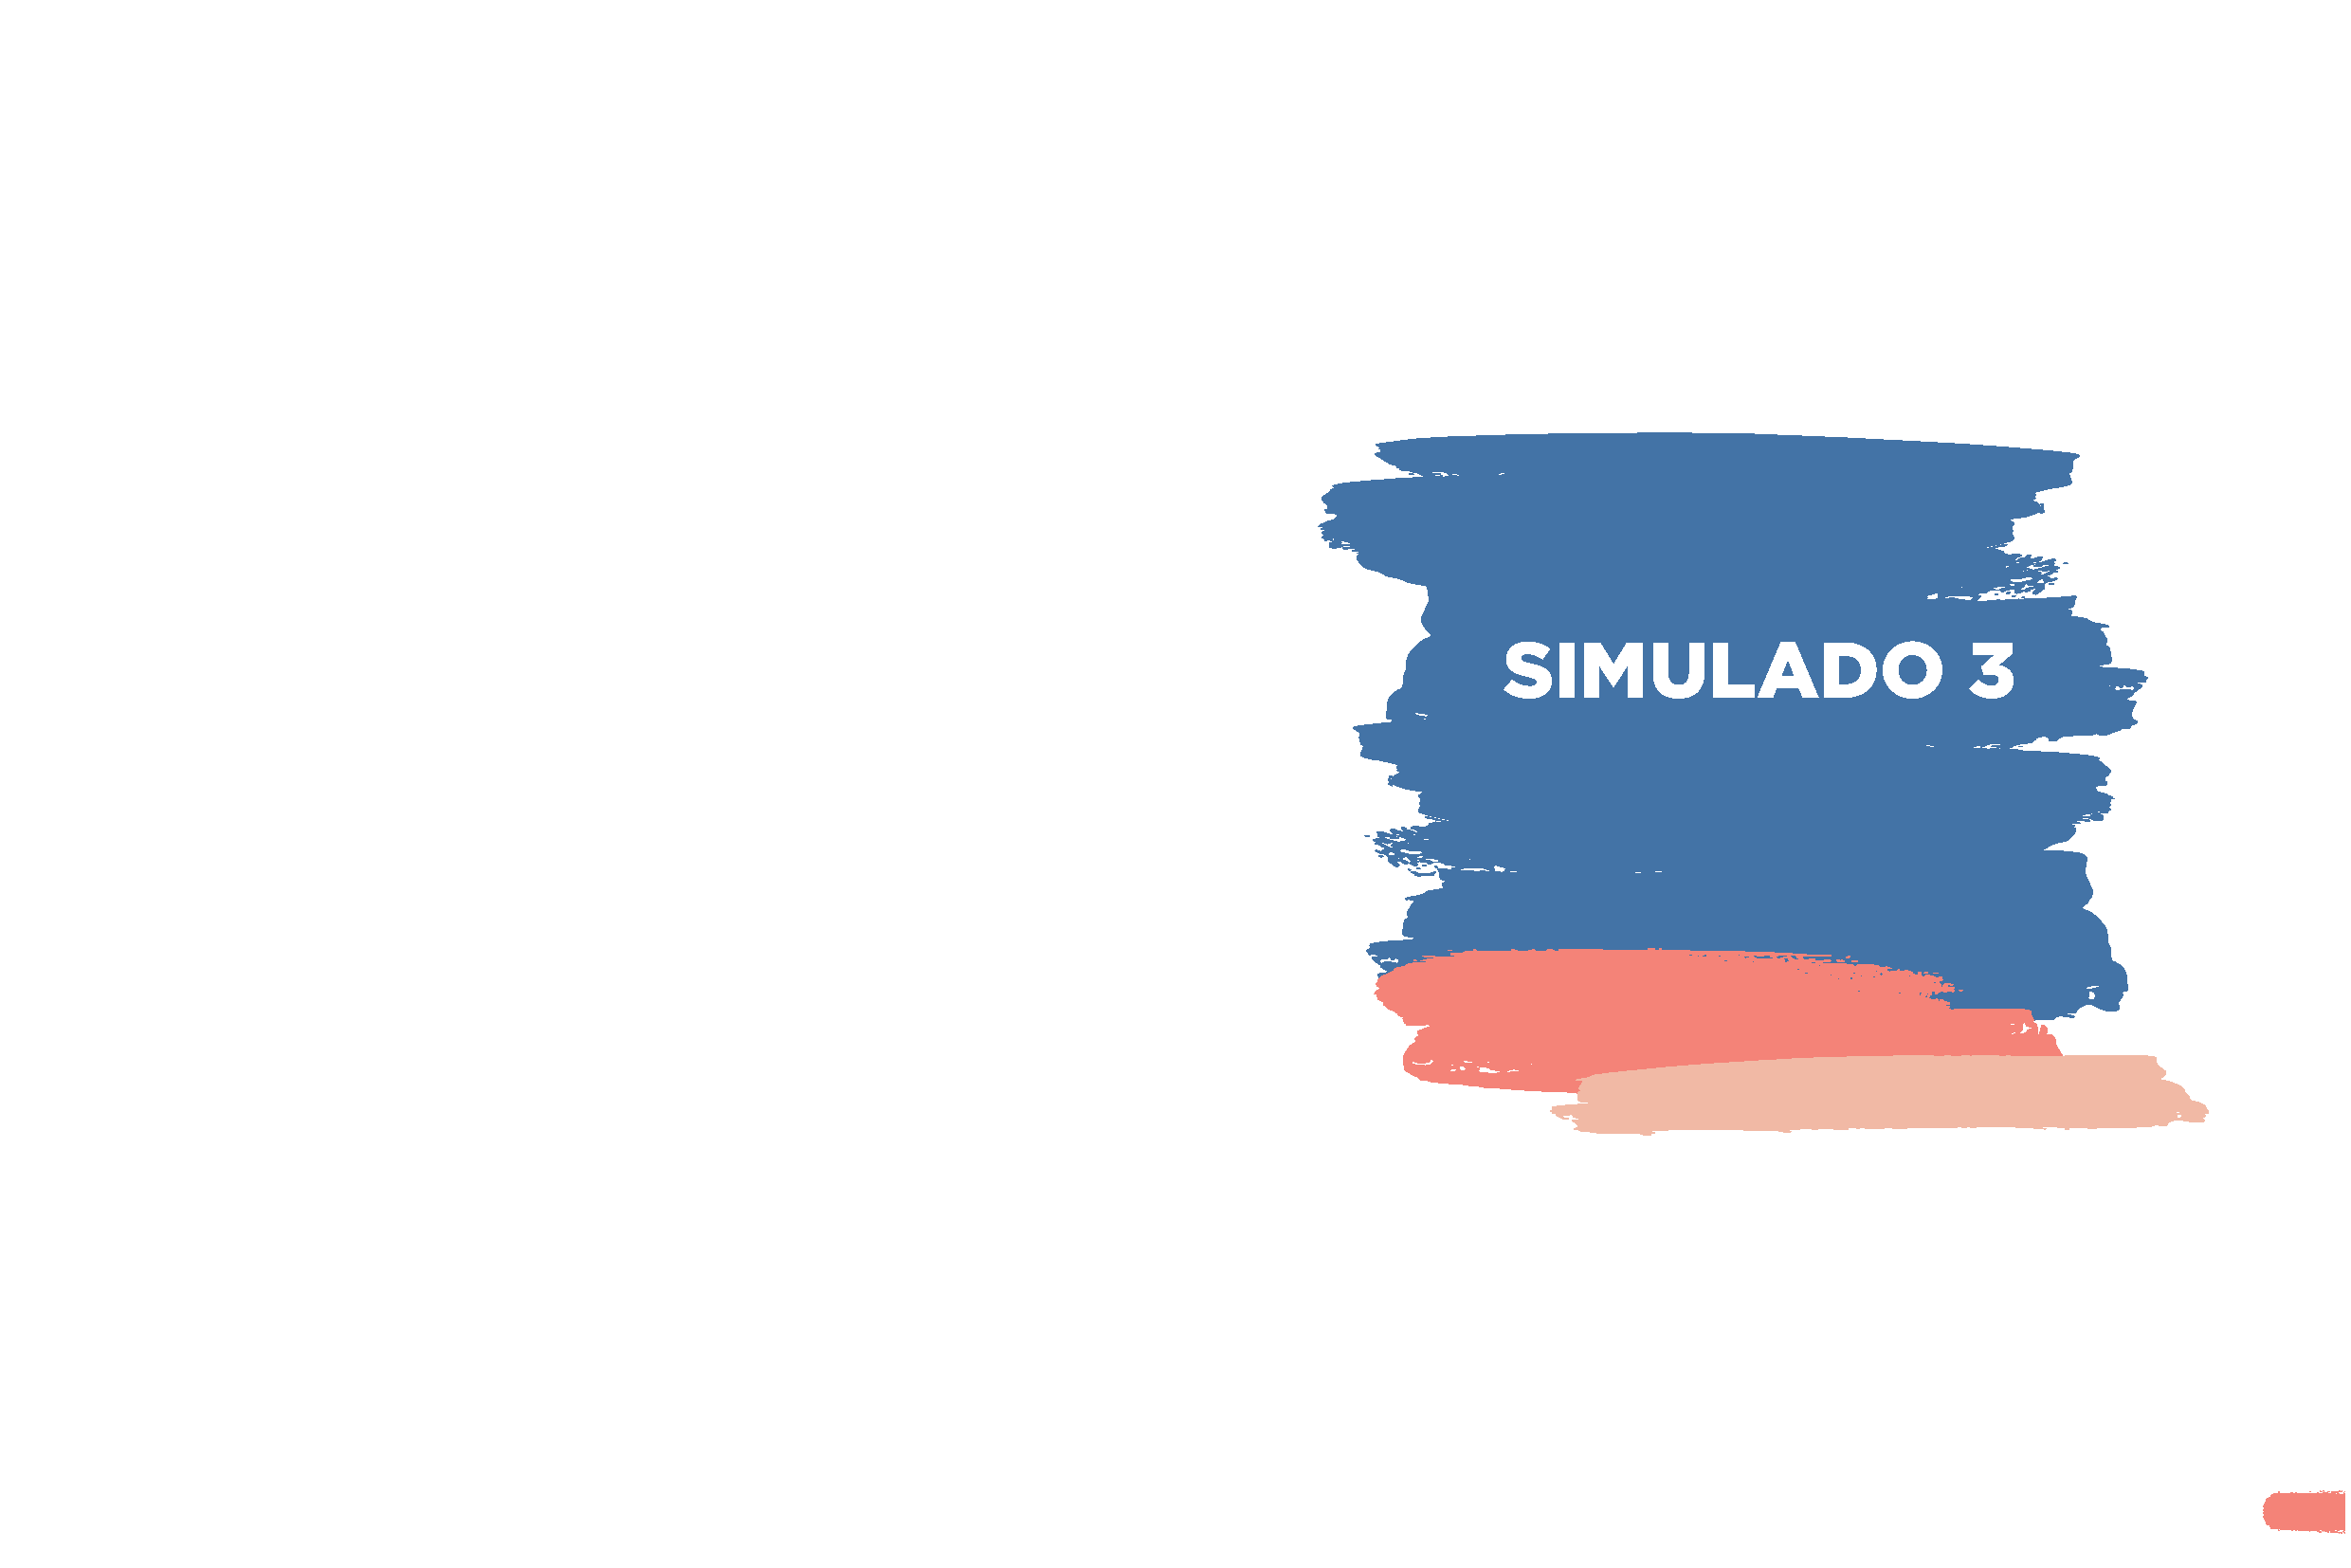
\includegraphics[scale=1]{../watermarks/3simulado5ano.pdf}
\addcontentsline{toc}{chapter}{Simulado 3}
\markboth{Simulado 3}{}

\pagebreak

\num{1} Durante a aula de matemática, a professora colocou na lousa a seguinte decomposição de um número:

\begin{myquote}
\centering
\textbf{4 x 1.000 + 3 x 100 + 3 x 10 + 5 x 1}
\end{myquote}

Muito rapidamente, Artur levantou a mão e disse que sabia qual era o número. Qual o número representado por essa decomposição?

\begin{escolha}
\item
  4.035.
\item
  4.335.
\item
  5.034.
\item
  5.304.
\end{escolha}

\num{2} Ricardo deseja escrever o maior número possível utilizando os algarismos 1, 2, 4, 5 e 7 sem repeti-los nenhuma vez. Qual é o número que ele irá escrever?

\begin{escolha}
\item
  Setecentos e cinquenta mil e quatrocentos e vinte um.
\item
  Setenta e cinco mil e quatrocentos e vinte um.
\item
  Quarenta e cinco mil e duzentos e cinquenta e sete.
\item
  Dezessete mil e quinhetos e quarenta e cinco.
\end{escolha}


\num{3} Cláudio separou 7 cubinhos e 6 barras do material dourado. Sendo assim, o maior número que ele conseguirá formar com essas peças será

\begin{multicols}{2}
\begin{escolha}
\item
  13.
\item
  76.
\item
  67.
\item
  21.
\end{escolha}
\end{multicols}

\num{4} Um grande circo chegou à cidade em que Rafael mora e logo uma fila enorme se formou com pessoas querendo assistir ao espetáculo. Os ingressos começaram a ser vendidos e as pessoas começaram a entrar. Em certo instante, sabia-se que 540 pessoas já tinham entrado e que a capacidade máxima por espetáculo nesse circo era de 1.200 pessoas. Como ainda temos 932 pessoas na fila, quantas pessoas não conseguirão entrar para assistir a essa seção do circo?

\begin{multicols}{2}
\begin{escolha}
\item
  660.
\item
  272.
\item
  268.
\item
  1.472.
\end{escolha}
\end{multicols}

\num{5} Alex estava observando a seguinte sequência numérica: 

\begin{myquote}
\centering
\textbf{3; 9; 27, 81; 243; 729.}
\end{myquote}

Pode-se dizer que, para encontrarmos um elemento qualquer da sequência, devemos 

\begin{multicols}{2}
\begin{escolha}
\item
  Somar 6 a um termo anterior.
\item
  Dividir por 3 um termo anterior.
\item
  Multiplicar por 3 um termo anterior.
\item
  Somar 9 a um termo anterior.
\end{escolha}
\end{multicols}

\num{6} O zoológico da cidade em que Fabiana mora abre às 9 horas da manhã e fica aberto apenas 8 horas e meia por dia. Qual o horário em que o zoológico fecha, sabendo-se que ele não fecha no horário do almoço?

\begin{escolha}
\item
  16 horas e trinta minutos.
\item
  17 horas e 30 minutos.
\item
  17 horas e 45 minutos.
\item
  18 horas e 30 minutos.
\end{escolha}

\pagebreak
\num{7} Para a festa de aniversário de Camila, sua avó preparou um bolo de um tamanho adequado para receber 25 convidados, mas, olhando novamente a lista, percebeu que iria receber mais do que 25 pessoas. Assim sendo, um bolo maior seria necessário.

O que a avó de Camila deverá fazer para ter um bolo que sirva adequadamente ao número de pessoas que irão à festa de aniversário de sua neta?

\begin{escolha}
\item
  Apenas comprar mais pratos descartáveis.
\item
  Aumentar a quantidade de alguns ingredientes.
\item
  Diminuir alguns ingredientes e aumentar outros.
\item
  Ampliar a quantidade de todos os ingredientes na mesma proporção inicial.
\end{escolha}


\num{8} Marina quer colocar um carpete de madeira no quarto de sua única filha.
Para isso, representou o quarto da menina numa malha quadriculada, onde a parte escura corresponde ao carpete de madeira que será
colocado.

\begin{figure}[htpb!]
\centering
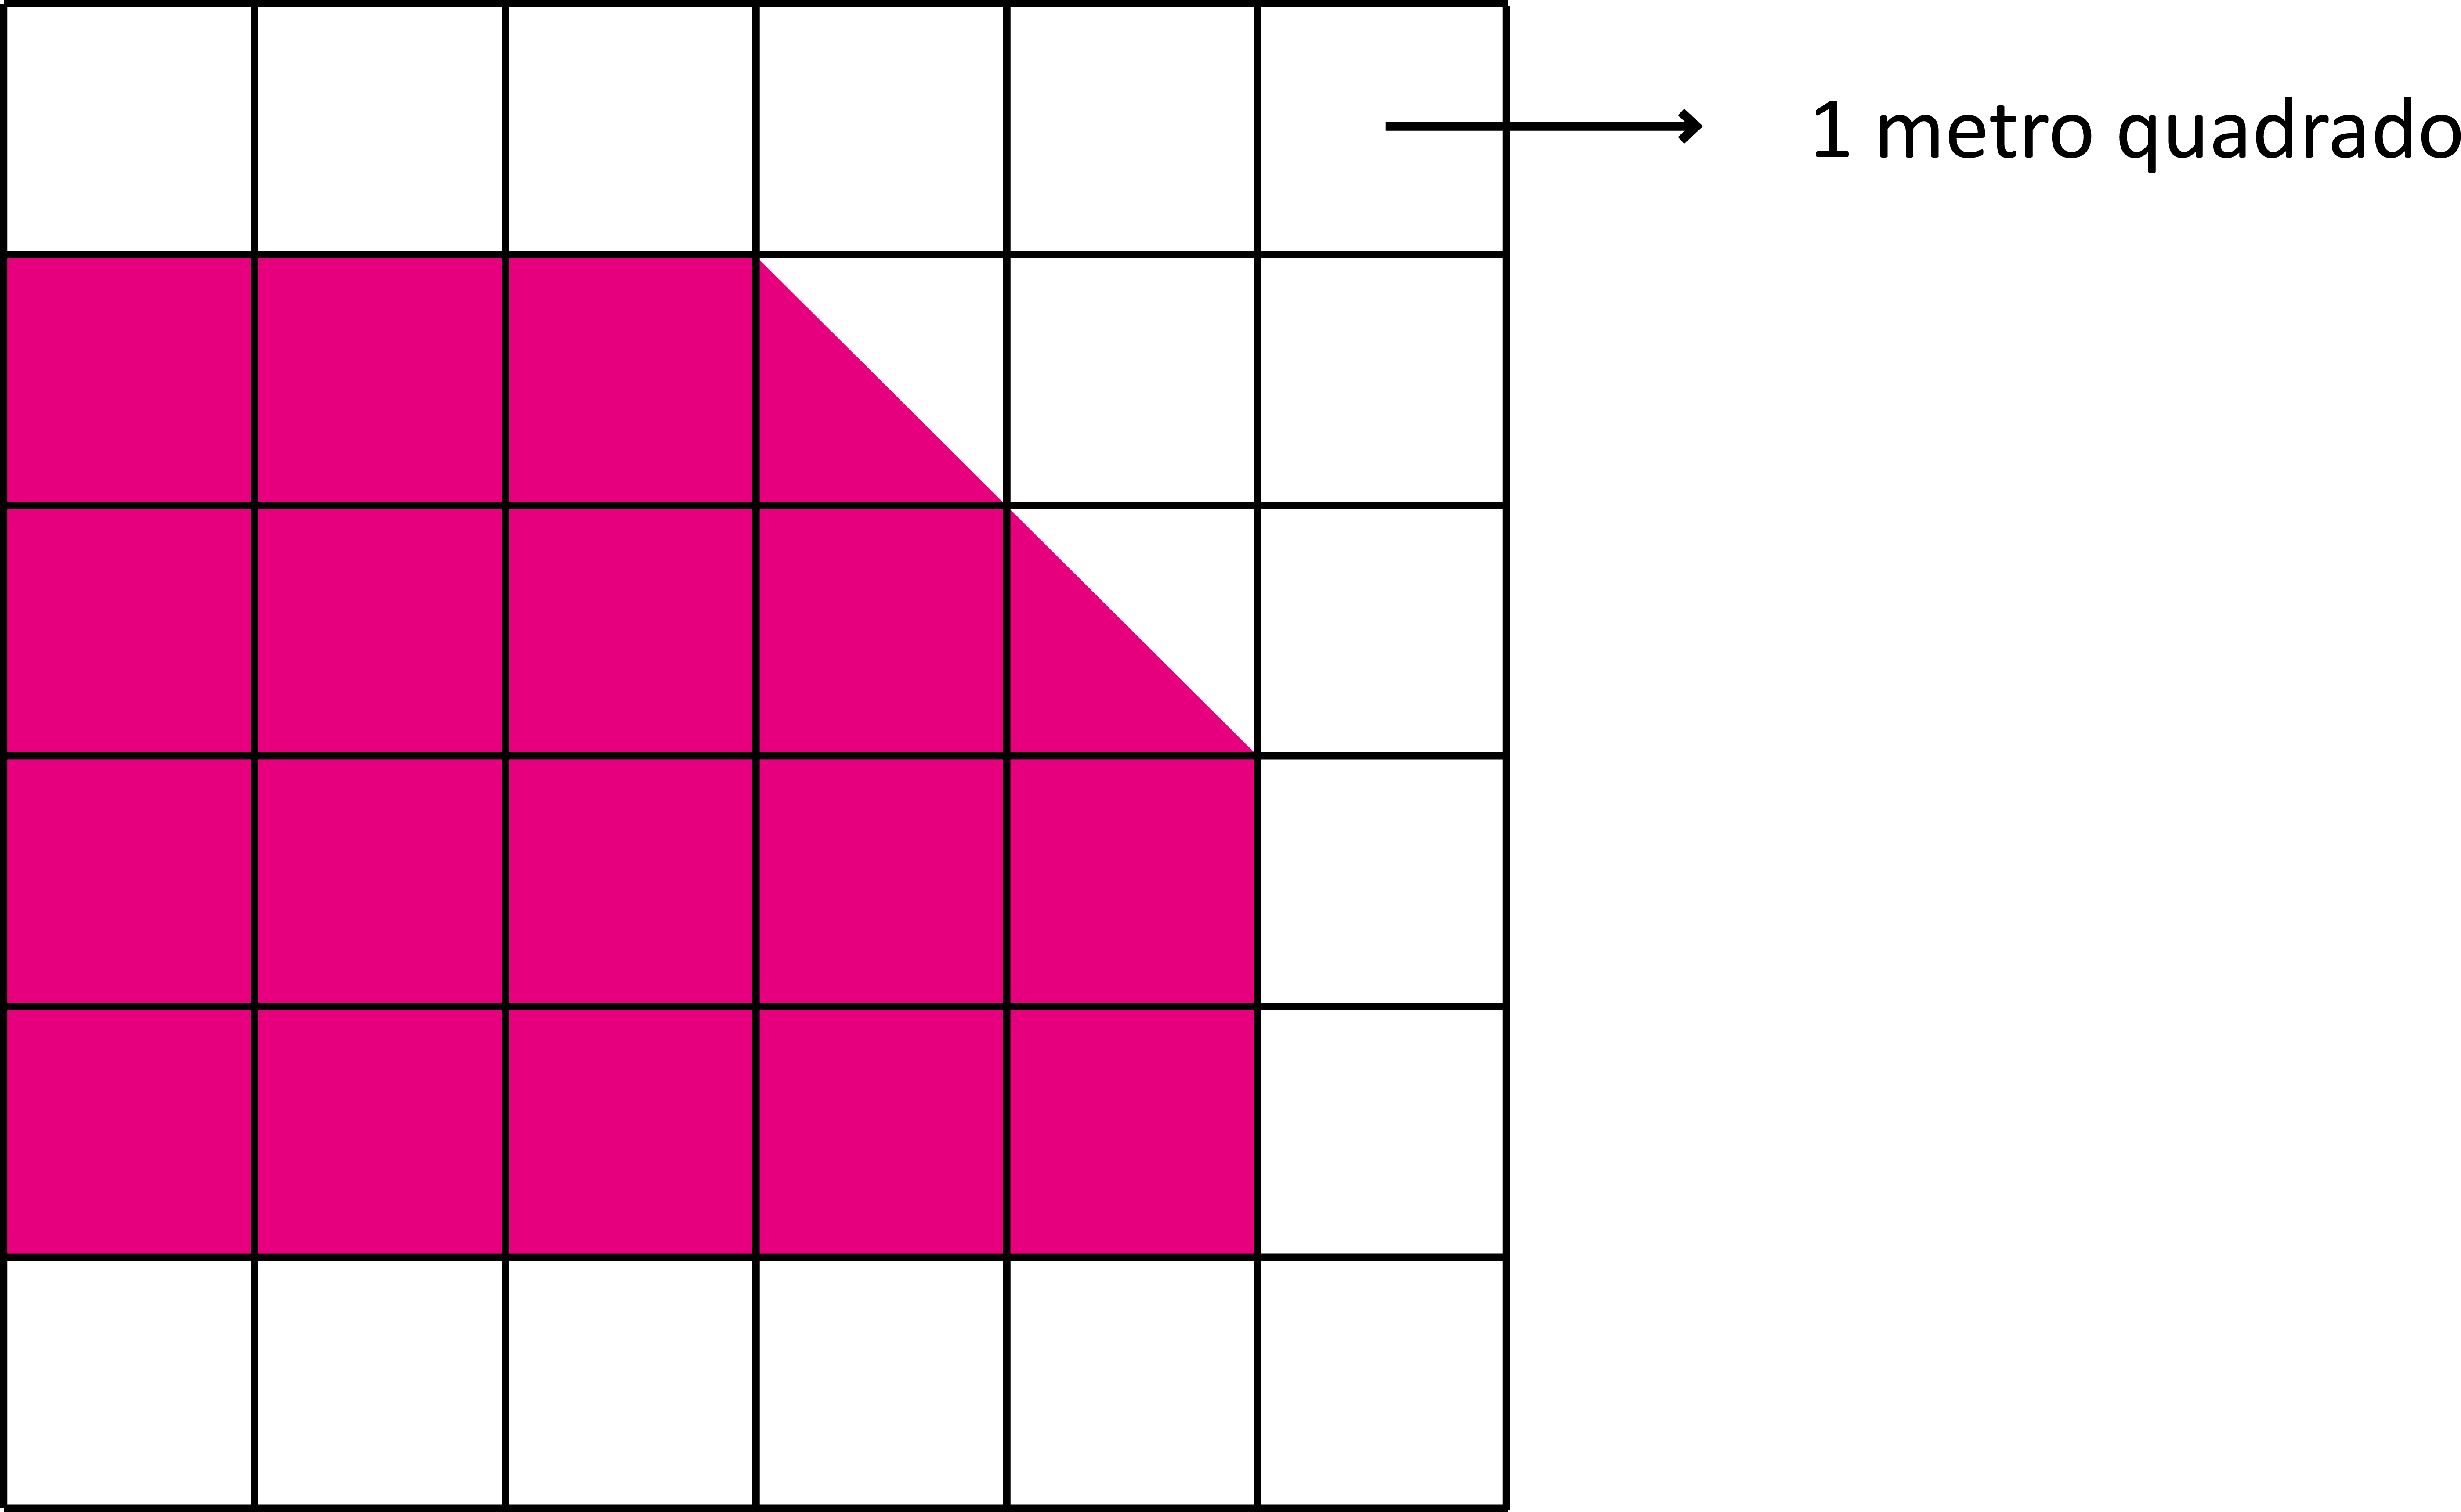
\includegraphics[width=.5\textwidth]{./media/image108.png}
\end{figure}

Como cada quadradinho possui 1 metro quadrado de área, qual a área total de carpete de madeira que ela terá que encomendar para colocar no quarto da filha sem que falte nenhum pedaço e também não sobre material?

\begin{multicols}{2}
\begin{escolha}
\item
  12 metros quadrados.
\item
  17 metros quadrados.
\item
  18 metros quadrados.
\item
  20 metros quadrados.
\end{escolha}
\end{multicols}

\num{9} Sara está montando uma biblioteca pessoal em sua casa. Ela possui 12 livros de romance, 6 de aventura e 14 de histórias em quadrinhos. Contando-se todos os livros, podemos afirmar que a biblioteca de Sara terá

\begin{multicols}{2}
\begin{escolha}
\item
  20 livros.
\item
  18 livros.
\item
  26 livros.
\item
  32 livros.
\end{escolha}
\end{multicols}

\num{10} Uma lanchonete construiu um gráfico sobre a quantidade de sanduíches
naturais vendidos em alguns dias.

\begin{figure}[htpb!]
\centering
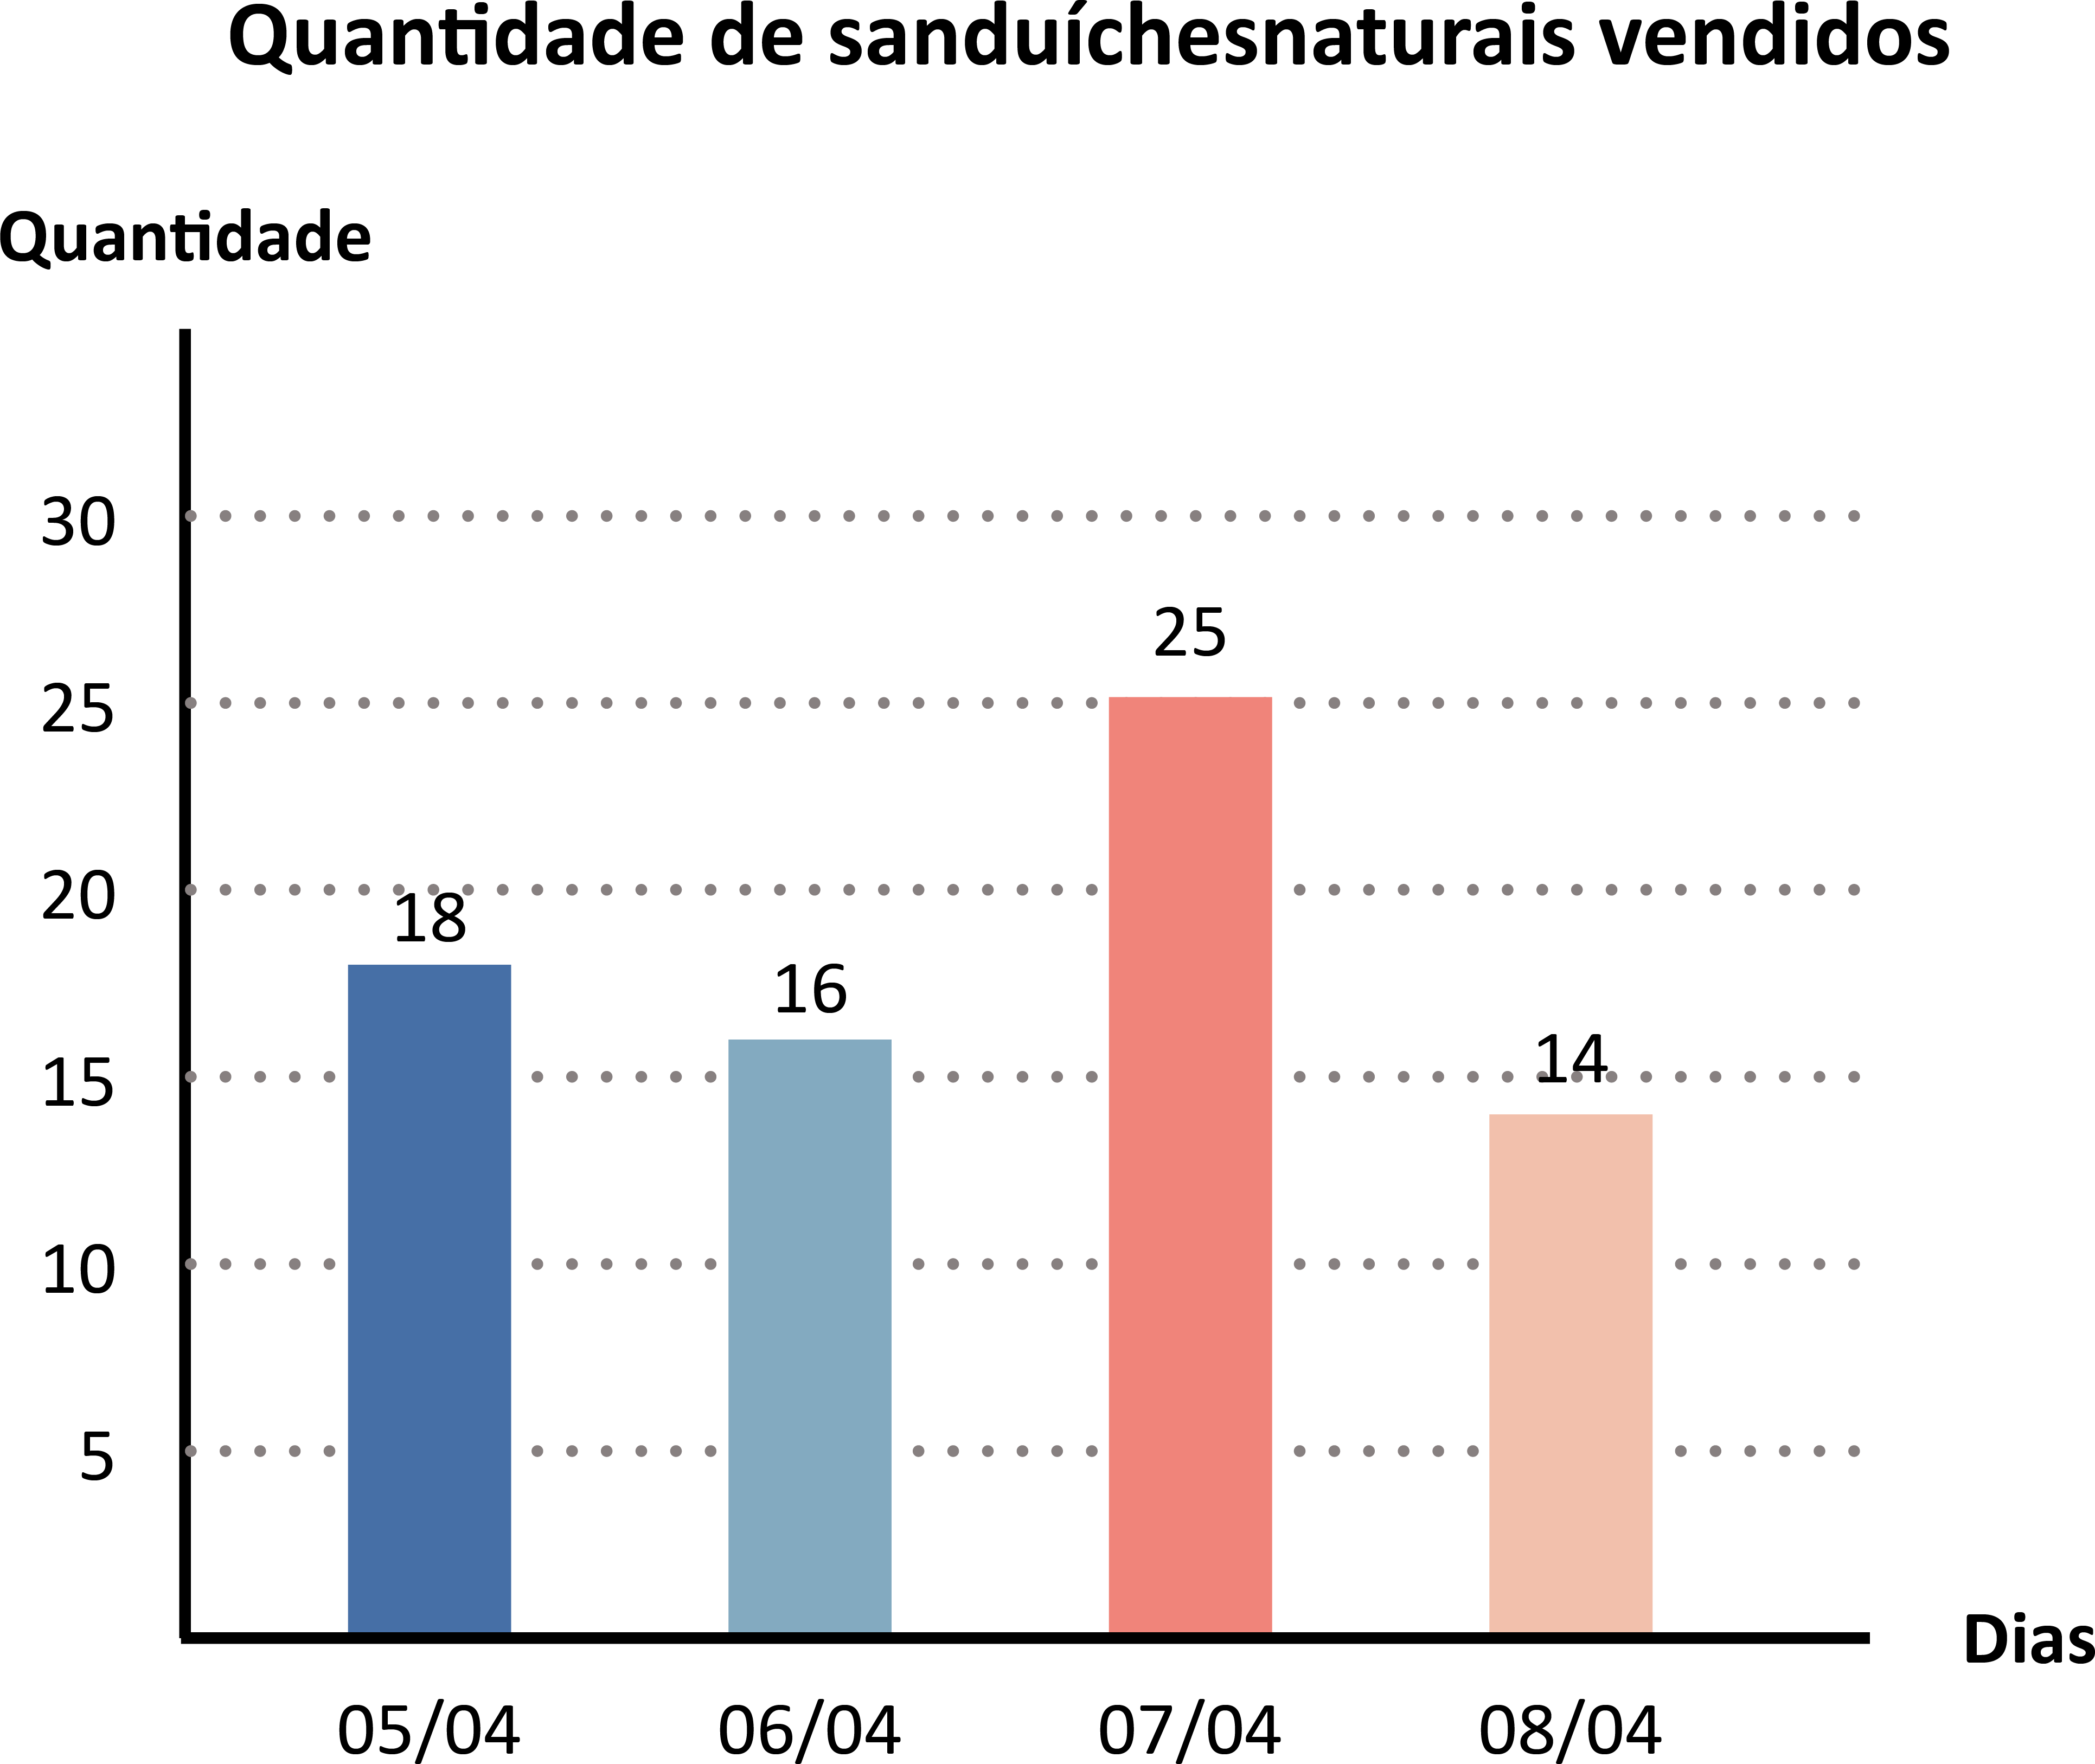
\includegraphics[width=0.7\textwidth]{./media/image109.png}
\end{figure}

Por meio da análise dos dados apresentados no gráfico, podemos concluir que o dia em que se teve a maior quantidade de vendas foi

\begin{multicols}{2}
\begin{escolha}
\item
  05/04.
\item
  06/04.
\item
  07/04.
\item
  08/04.
\end{escolha}
\end{multicols}

\num{11} Letícia resolveu arrumar as coisas que estavam em sua bolsa e encontrou os seguintes valores:

\begin{figure}[htpb!]
\centering
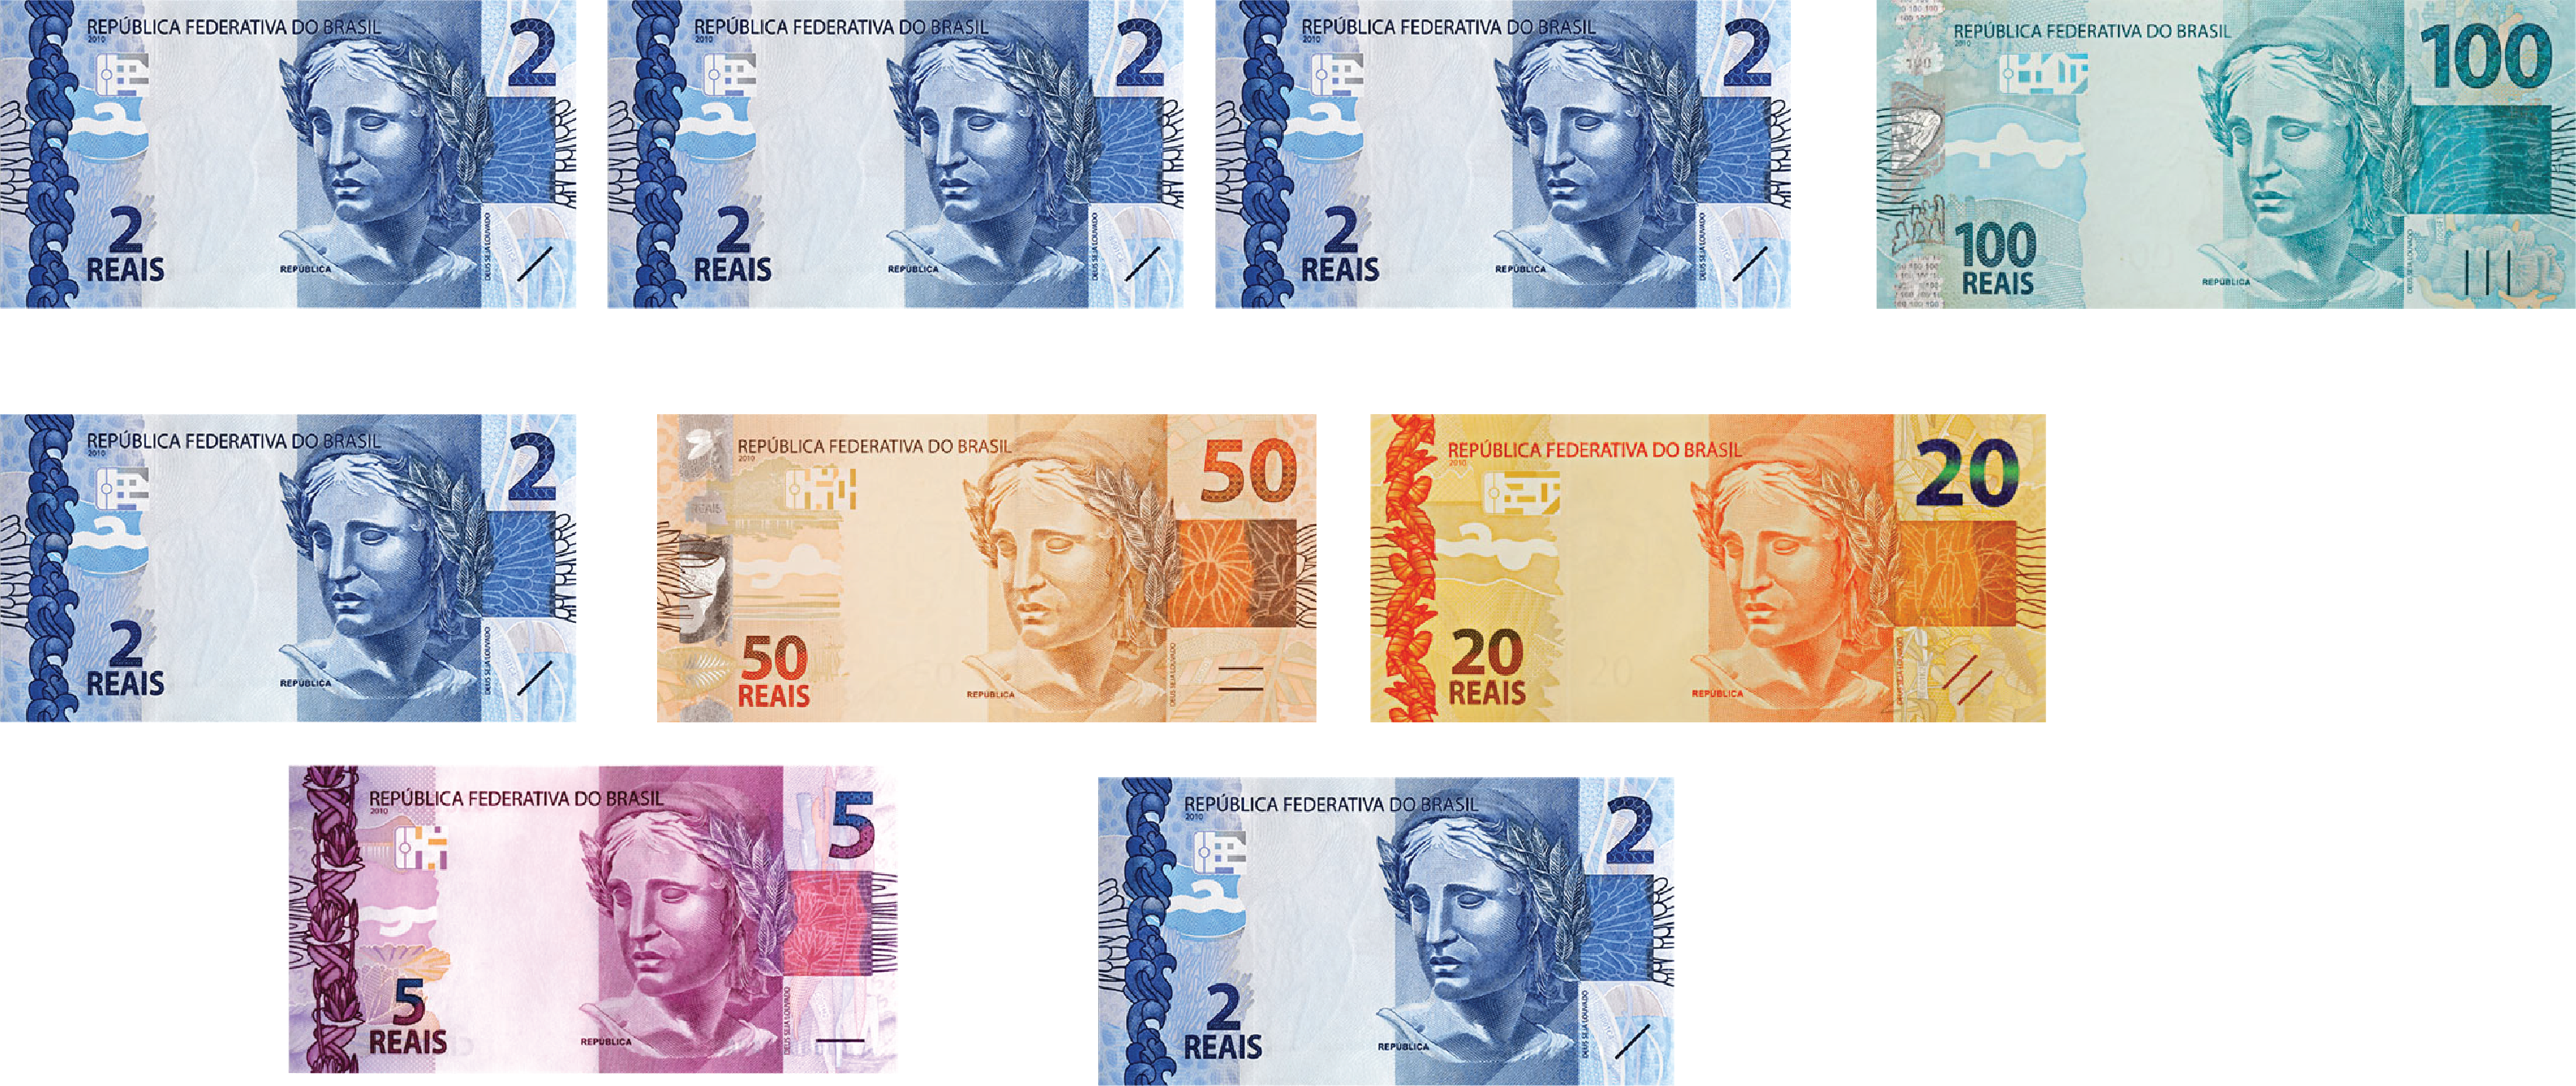
\includegraphics[width=0.7\textwidth]{./media/image110.png}
\end{figure}

Após uma contagem rápida ela concluiu que possuía em sua bolsa a quantia de

\begin{escolha}
\item
  R\$ 136,00.
\item
  R\$ 149,00.
\item
  R\$ 185,00.
\item
  R\$ 200,00.
\end{escolha}


\num{12} Maria está assando um bolo para sua filha e disse que ele ficará pronto às 3 horas e 25 minutos da tarde.

O relógio que traz a hora correta em que o bolo ficará pronto é:

\begin{figure}[htpb!]
\centering
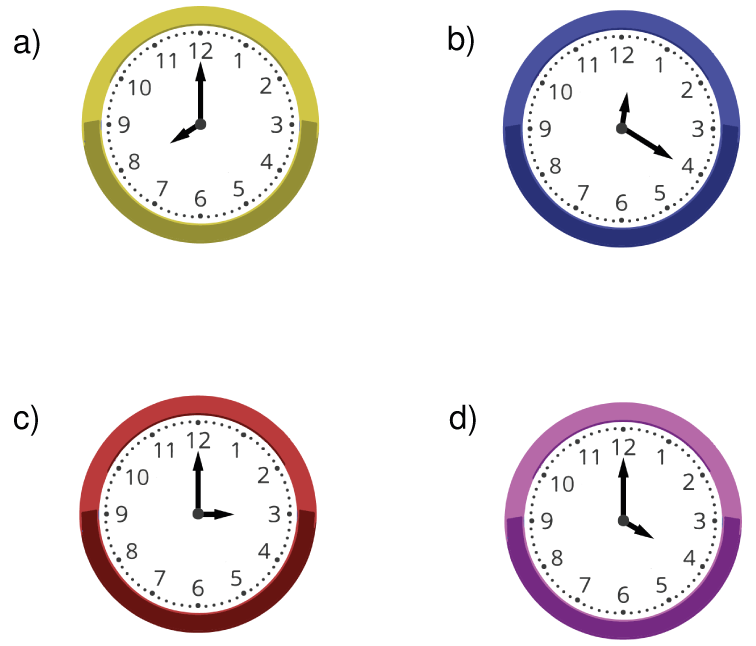
\includegraphics[width=.45\textwidth]{./media/image111.png}
\end{figure}
%NOTE. Verificar se a imagem final apresenta as alternativas.

\pagebreak
\num{13} Foi feito um levantamento sobre o tempo de vida, aproximado, em anos, de alguns animais e os dados foram colocados no seguinte gráfico:

\begin{figure}[htpb!]
\centering
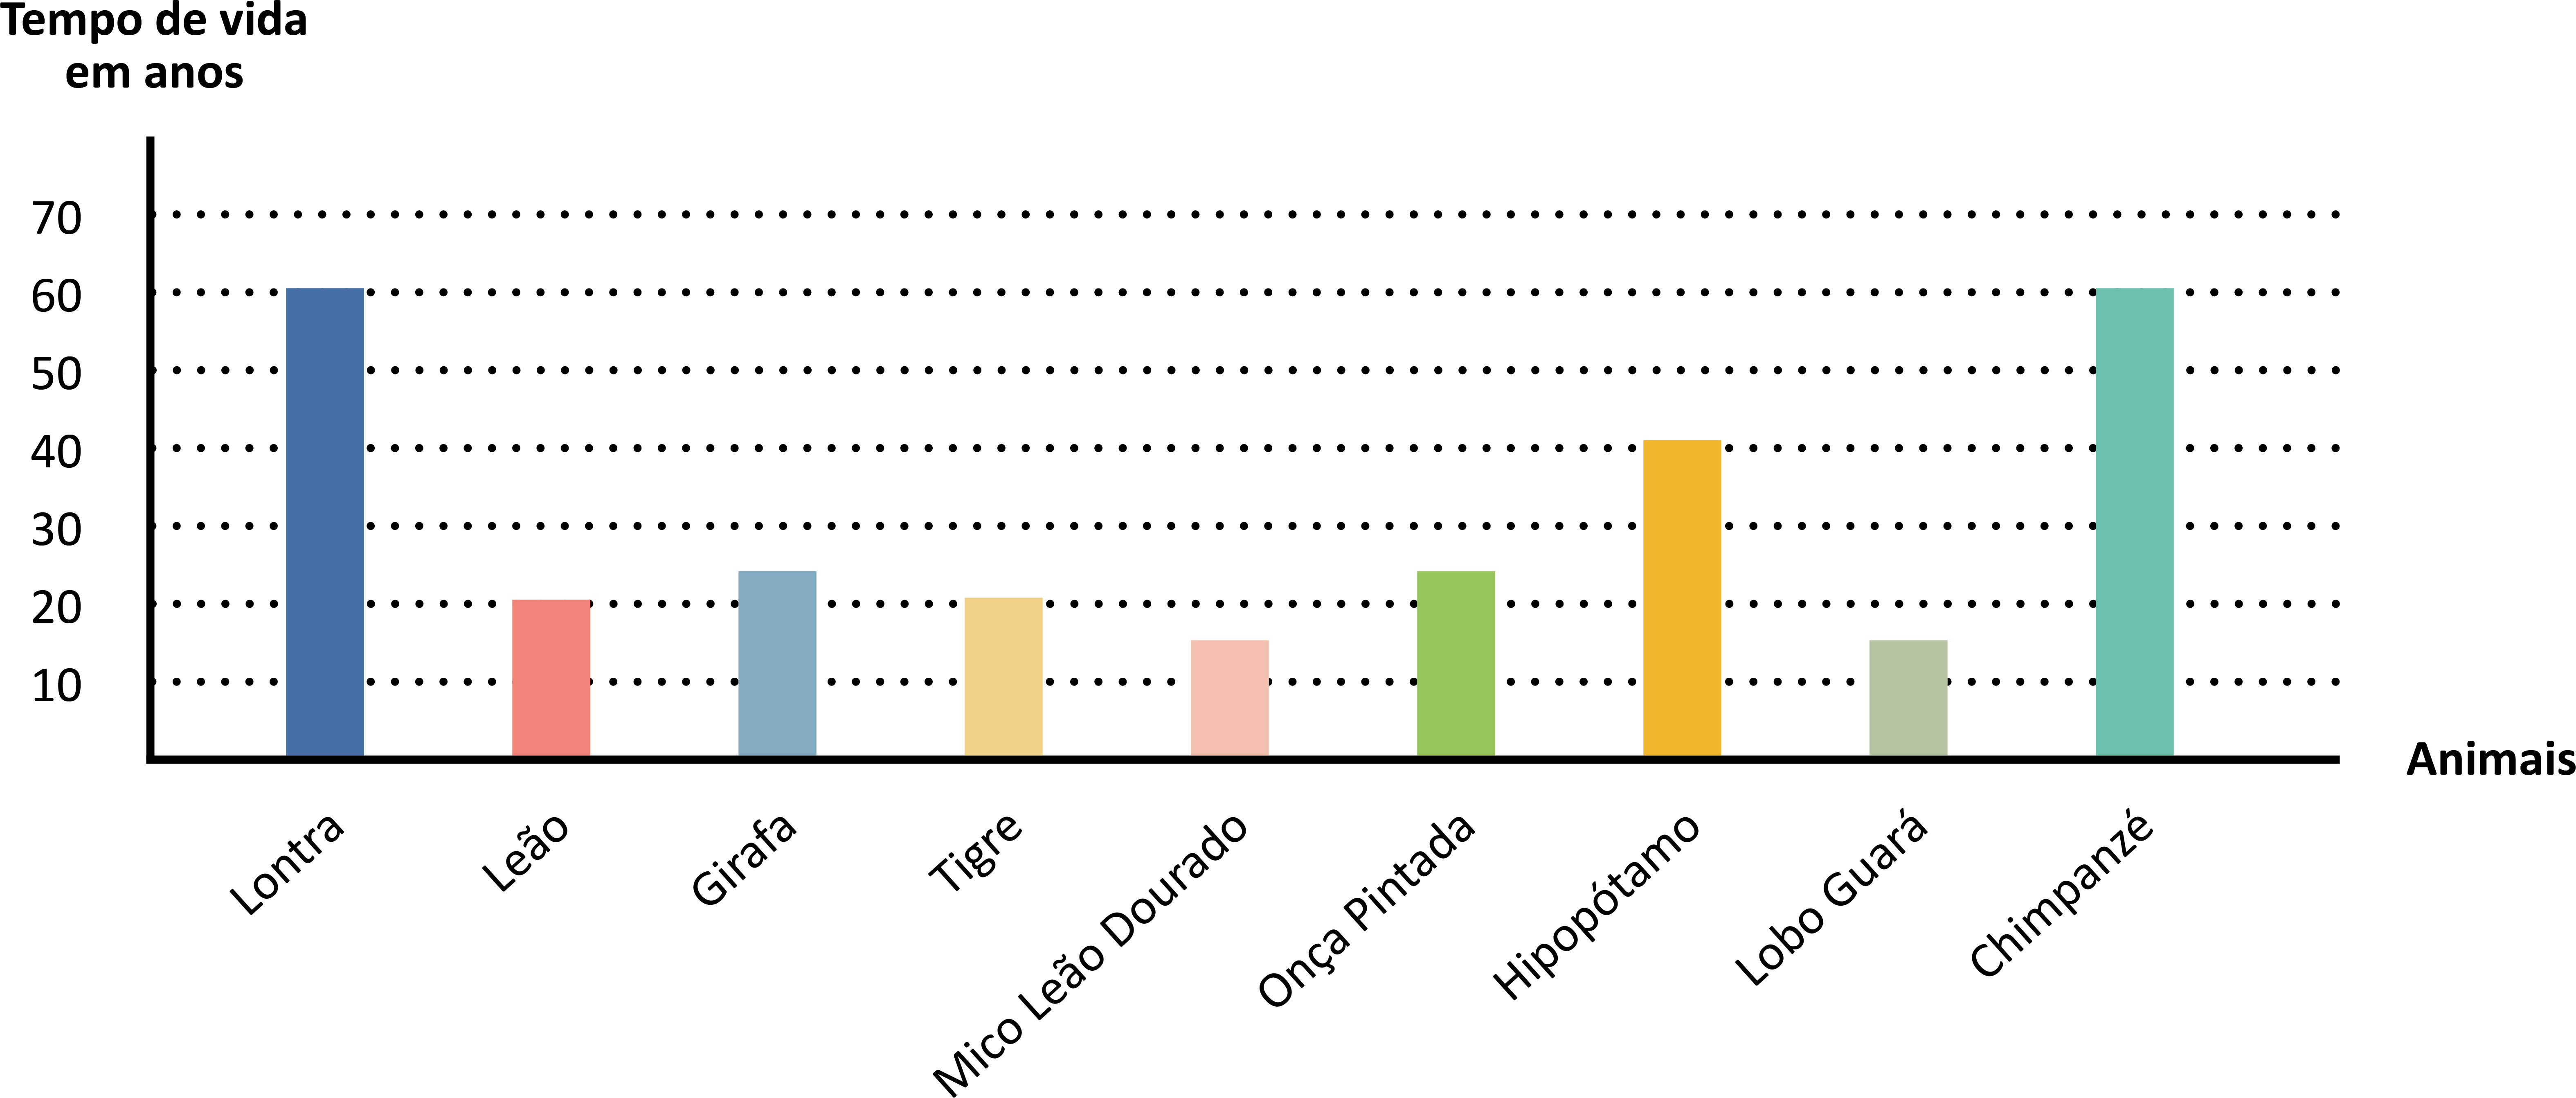
\includegraphics[width=\textwidth]{./media/image112.png}
\end{figure}

Analisando atentamete o gráfico, pode-se afirmar que os animais que vivem menos que o tigre e o leão são

\begin{multicols}{2}[\setlength{\columnsep}{-1cm}]
\begin{escolha}
\item
  Lontra e chimpanzé.
\item
  Hipopótamo e Girafa.
\item
  Mico-leão-dourado e lobo-guará.
\item
  Lontra e Mico-leão-dourado.
\end{escolha}
\end{multicols}


\num{14} Seis alunos foram à secretaria da escola e pegaram 8 folhas de sulfite cada um. Essas folhas serão para realizarem um trabalho em grupo. Sabendo-se que os 6 alunos que foram buscar as folhas são do mesmo grupo
e que não desperdiçaram nenhuma folha, conclui-se que o trabalho terá, no total

\begin{multicols}{2}
\begin{escolha}
\item
  8 folhas.
\item
  6 folhas.
\item
  14 folhas.
\item
  48 folhas.
\end{escolha}
\end{multicols}

\pagebreak

\num{15} Quatro amigos resolveram realizar uma medida das suas respectivas massas corpóreas. Veja a imagem de cada uma das balanças.

\begin{figure}[htpb!]
\centering
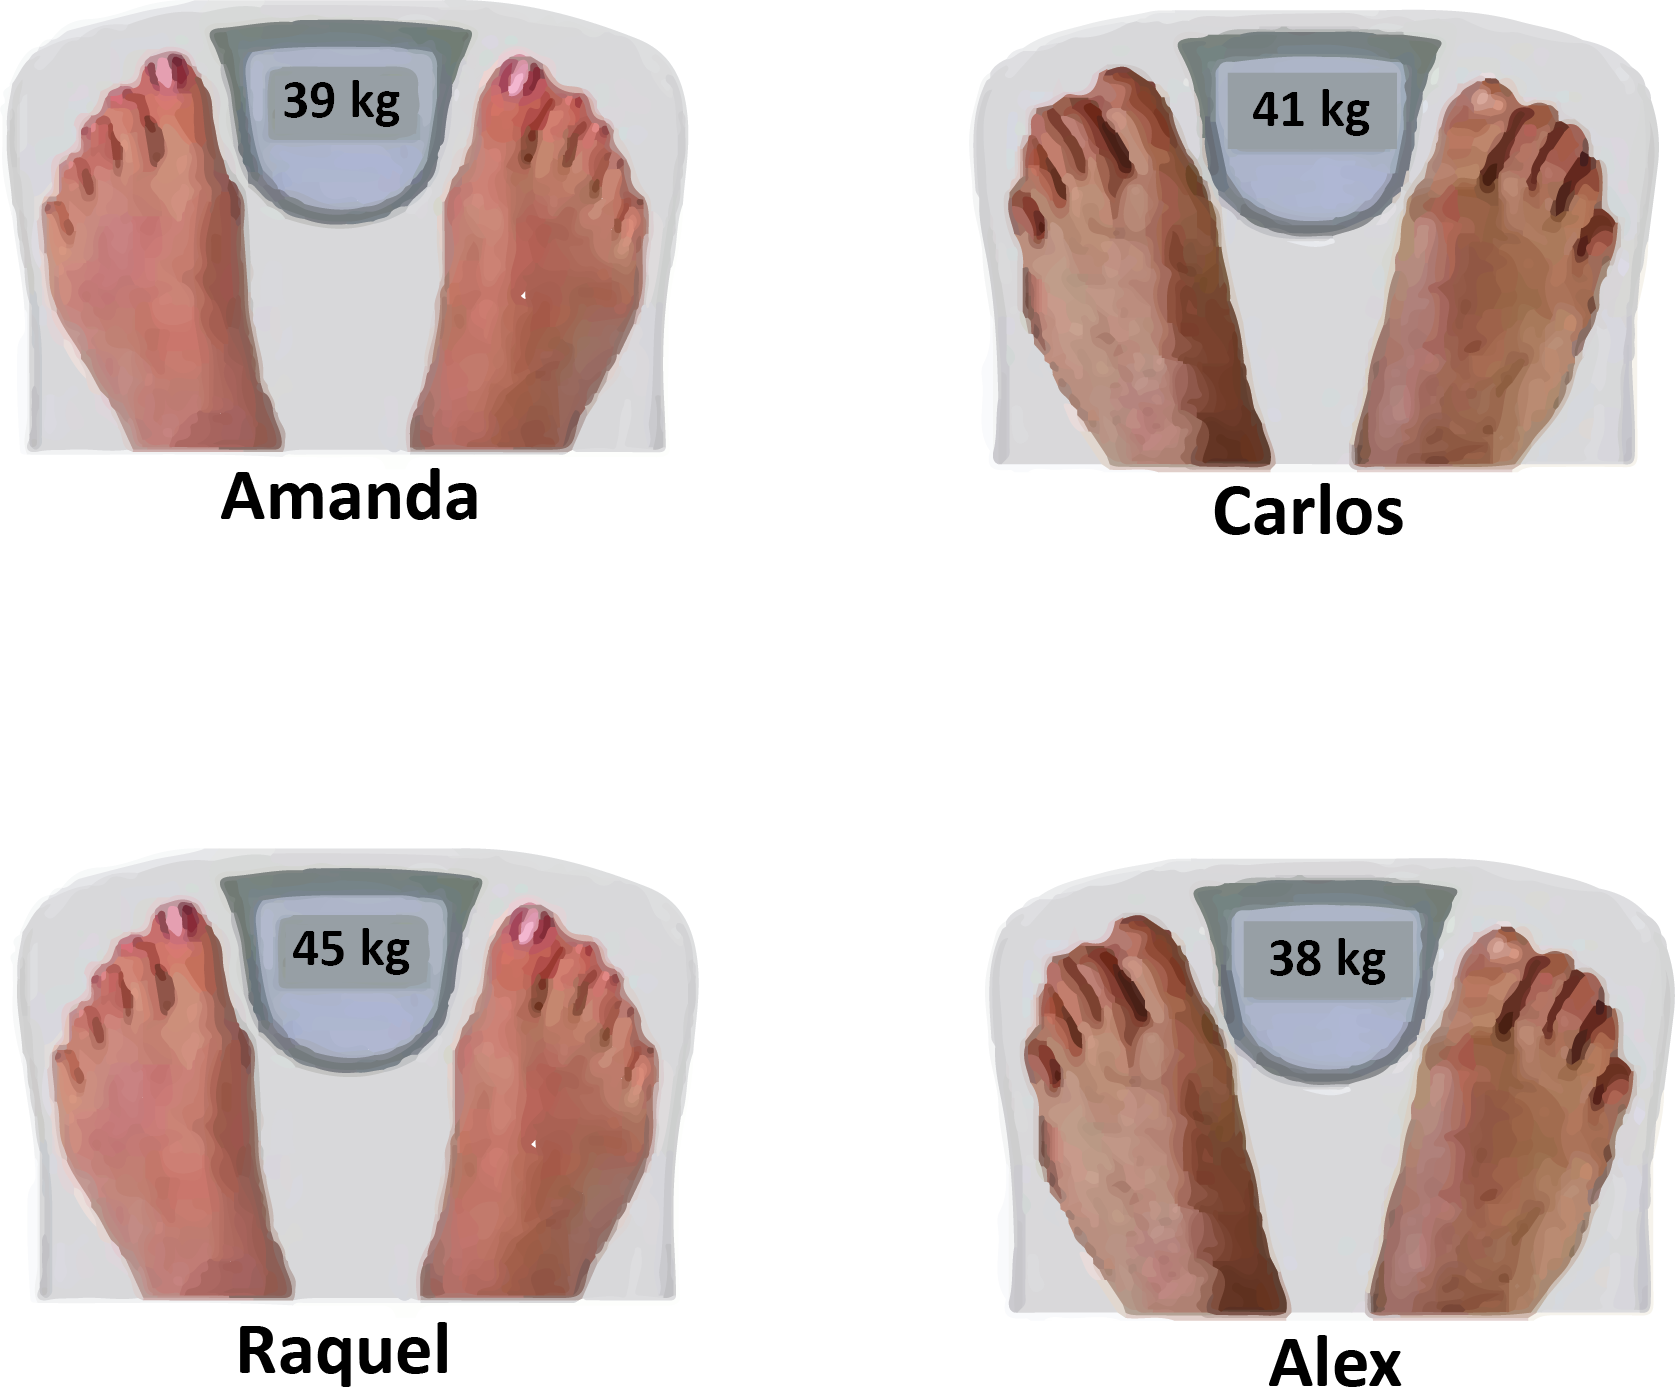
\includegraphics[width=.8\textwidth]{./media/image113.png}
\end{figure}

Observando as imagens das balanças, pode-se afirmar que a pessoa que apresenta a maior massa é

%\begin{multicols}{2}
\begin{escolha}
\item
  Amanda.
\item
  Raquel.
\item
  Carlos.
\item
  Alex.
\end{escolha}
%\end{multicols}
%NOTE. INVERTER GABARITO 14 pelo 15
\pagebreak

\vspace*{-3.4cm}
%\hspace*{-3.7cm}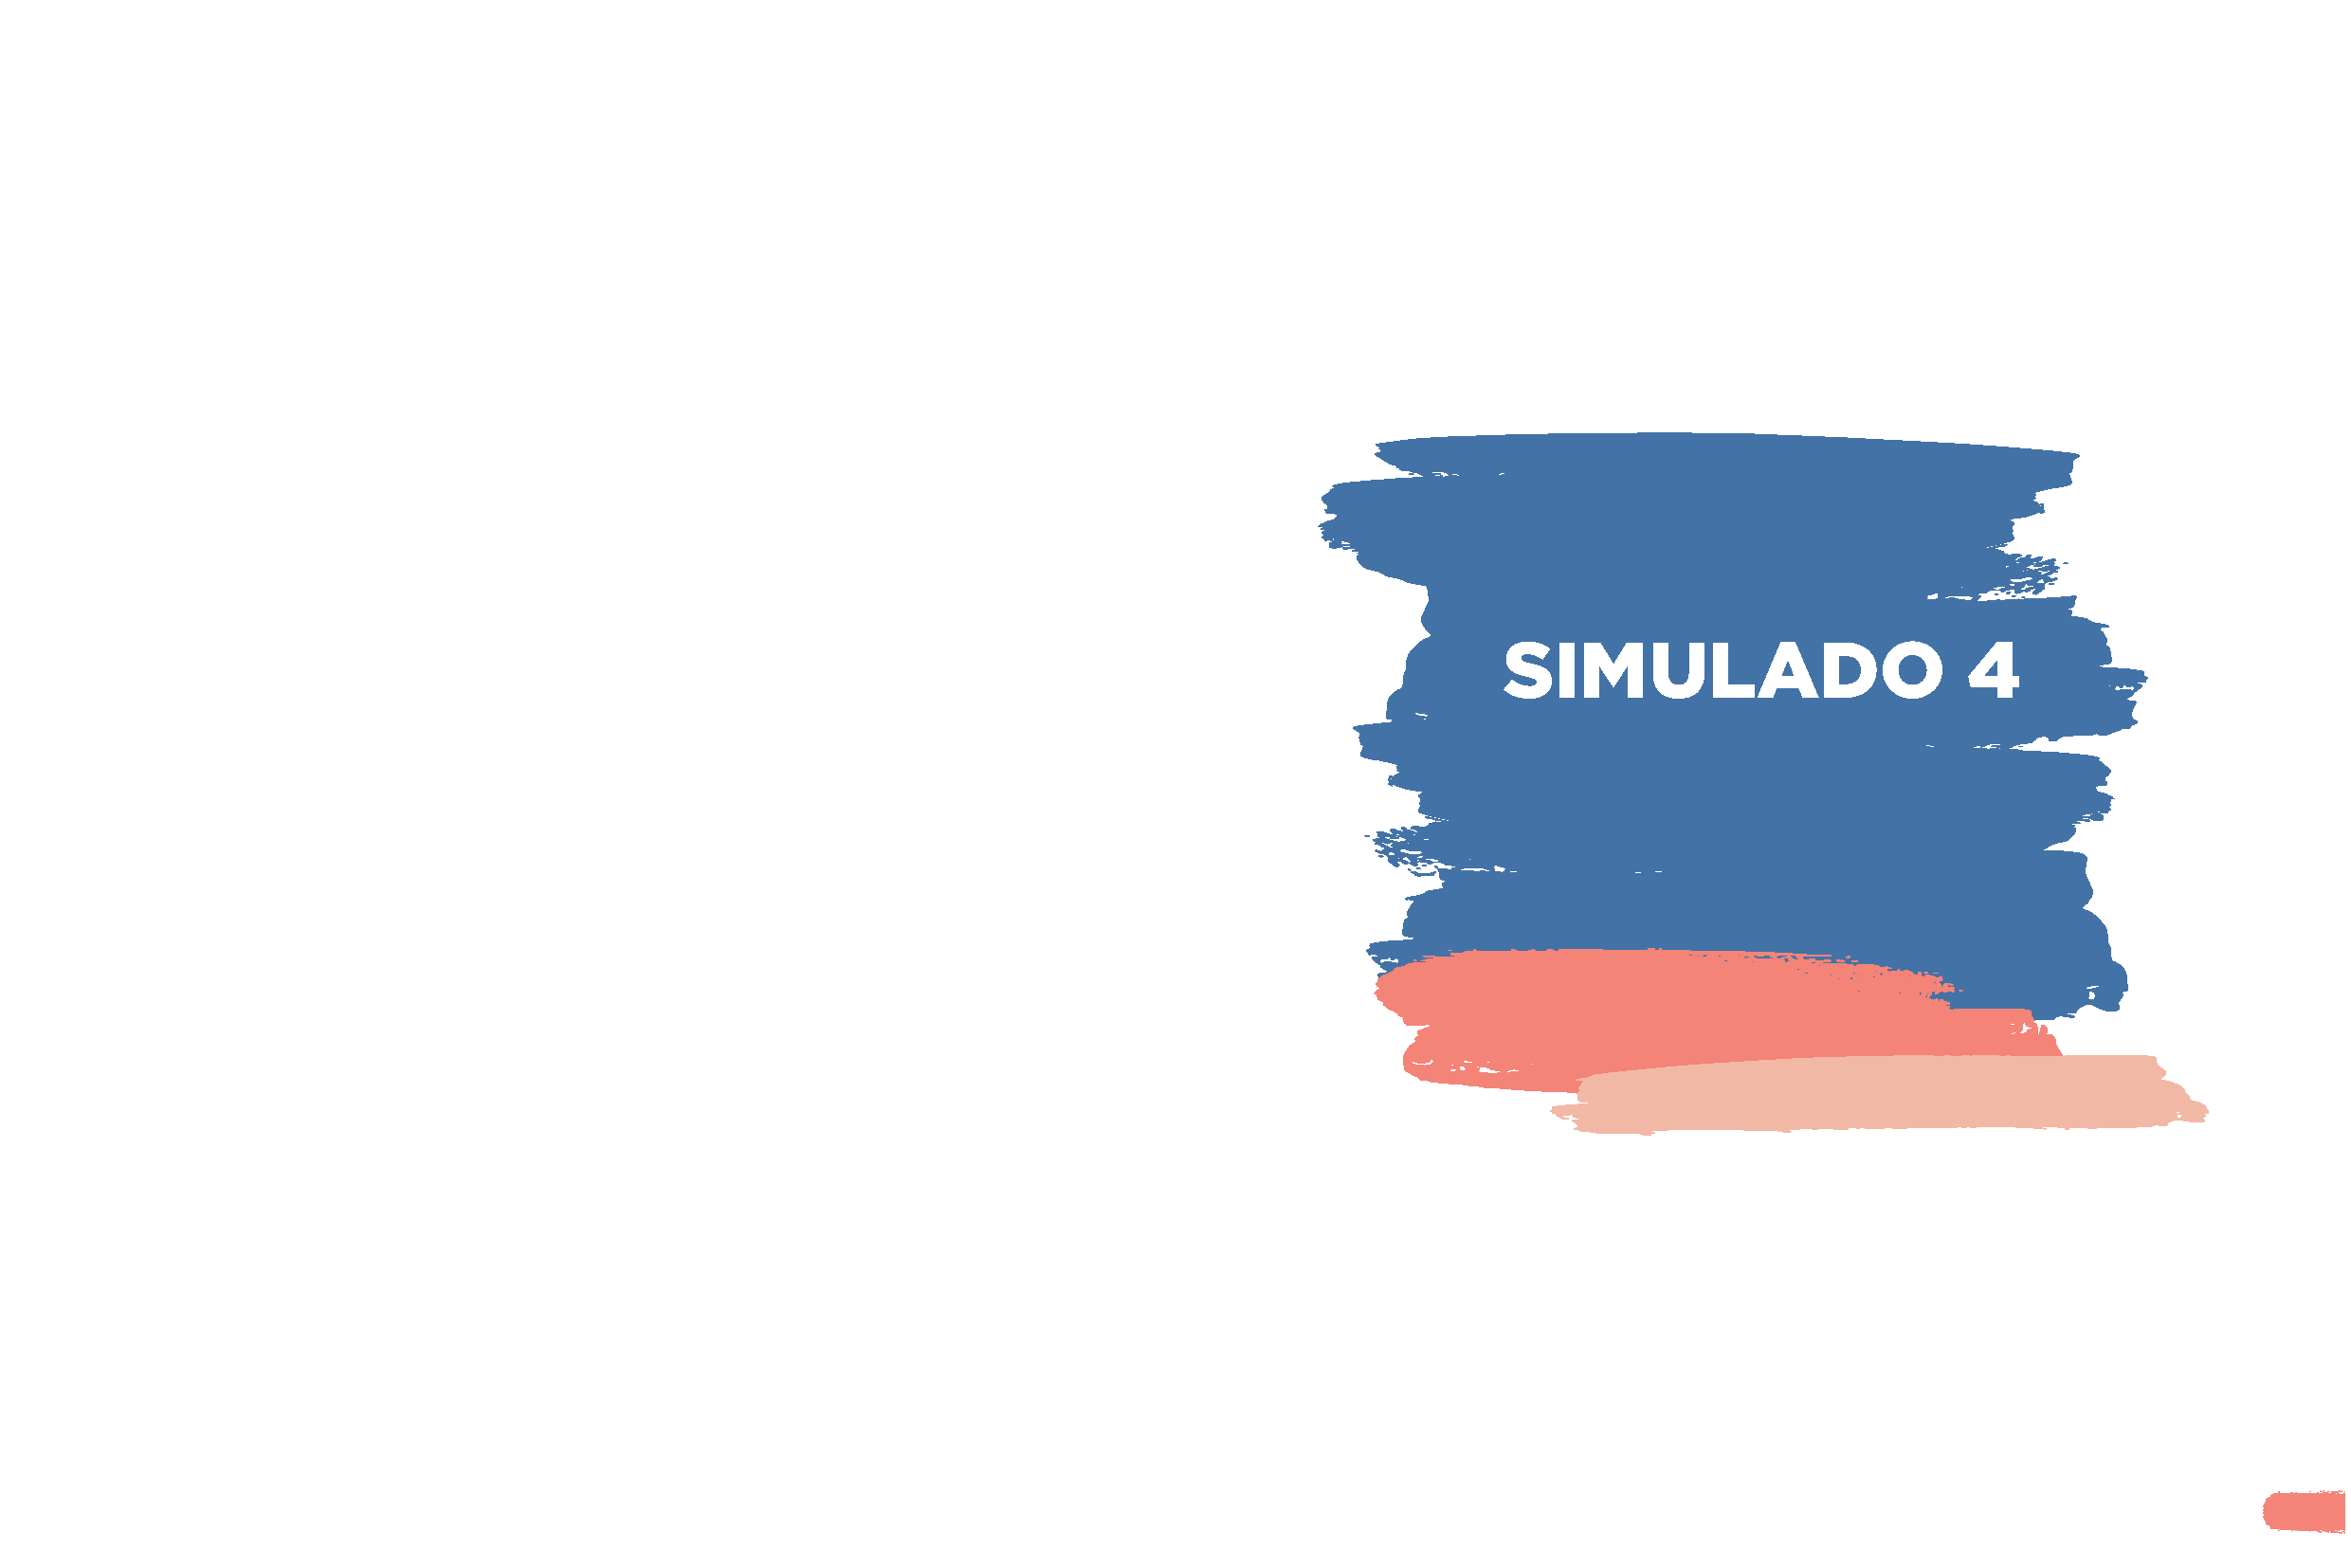
\includegraphics[scale=1]{../watermarks/4simulado5ano.pdf}
\addcontentsline{toc}{chapter}{Simulado 4}
\markboth{Simulado 4}{}

\pagebreak

\num{1} Um jogo consiste em uma pessoa sortear um número e, após ver qual número foi, pensar por alguns instantes e dizer em qual potinho deve ser colocado cada algarismo do número.


O número que acabou de ser sorteado foi 3.756. Qual o algarismo que será colocado no potinho com rótulo centenas?

\begin{escolha}
\item
  7.
\item
  6.
\item
  5.
\item
  3.
\end{escolha}

\num{2} Fred foi comemorar a promoção que recebeu de seu chefe em uma pizzaria. Inicialmente, resolveram pedir 2 pizzas e perceberam que o valor total seria de R\$ 81,60. Se após alguns cálculos resolvessem comprar 6
pizzas, o valor pago seria de


\begin{escolha}
\item
  R\$ 40,80.
\item
  R\$ 81,60.
\item
  R\$ 122,40.
\item
  R\$ 244,80.
\end{escolha}


\num{3} Henrique leu hoje 60 páginas de um livro. Podemos afirmar que o número de dezenas que ele leu hoje foi de

\begin{multicols}{2}
\begin{escolha}
\item
  4
\item
  5
\item
  6
\item
  7
\end{escolha}
\end{multicols}

\pagebreak
\num{4} A mãe de Joana está fazendo uma deliciosa salada de frutas e para terminar só falta colocar uva e morango. A quantidade de cada uma dessas frutas está representada na imagem.

\begin{figure}[htpb!]
\centering
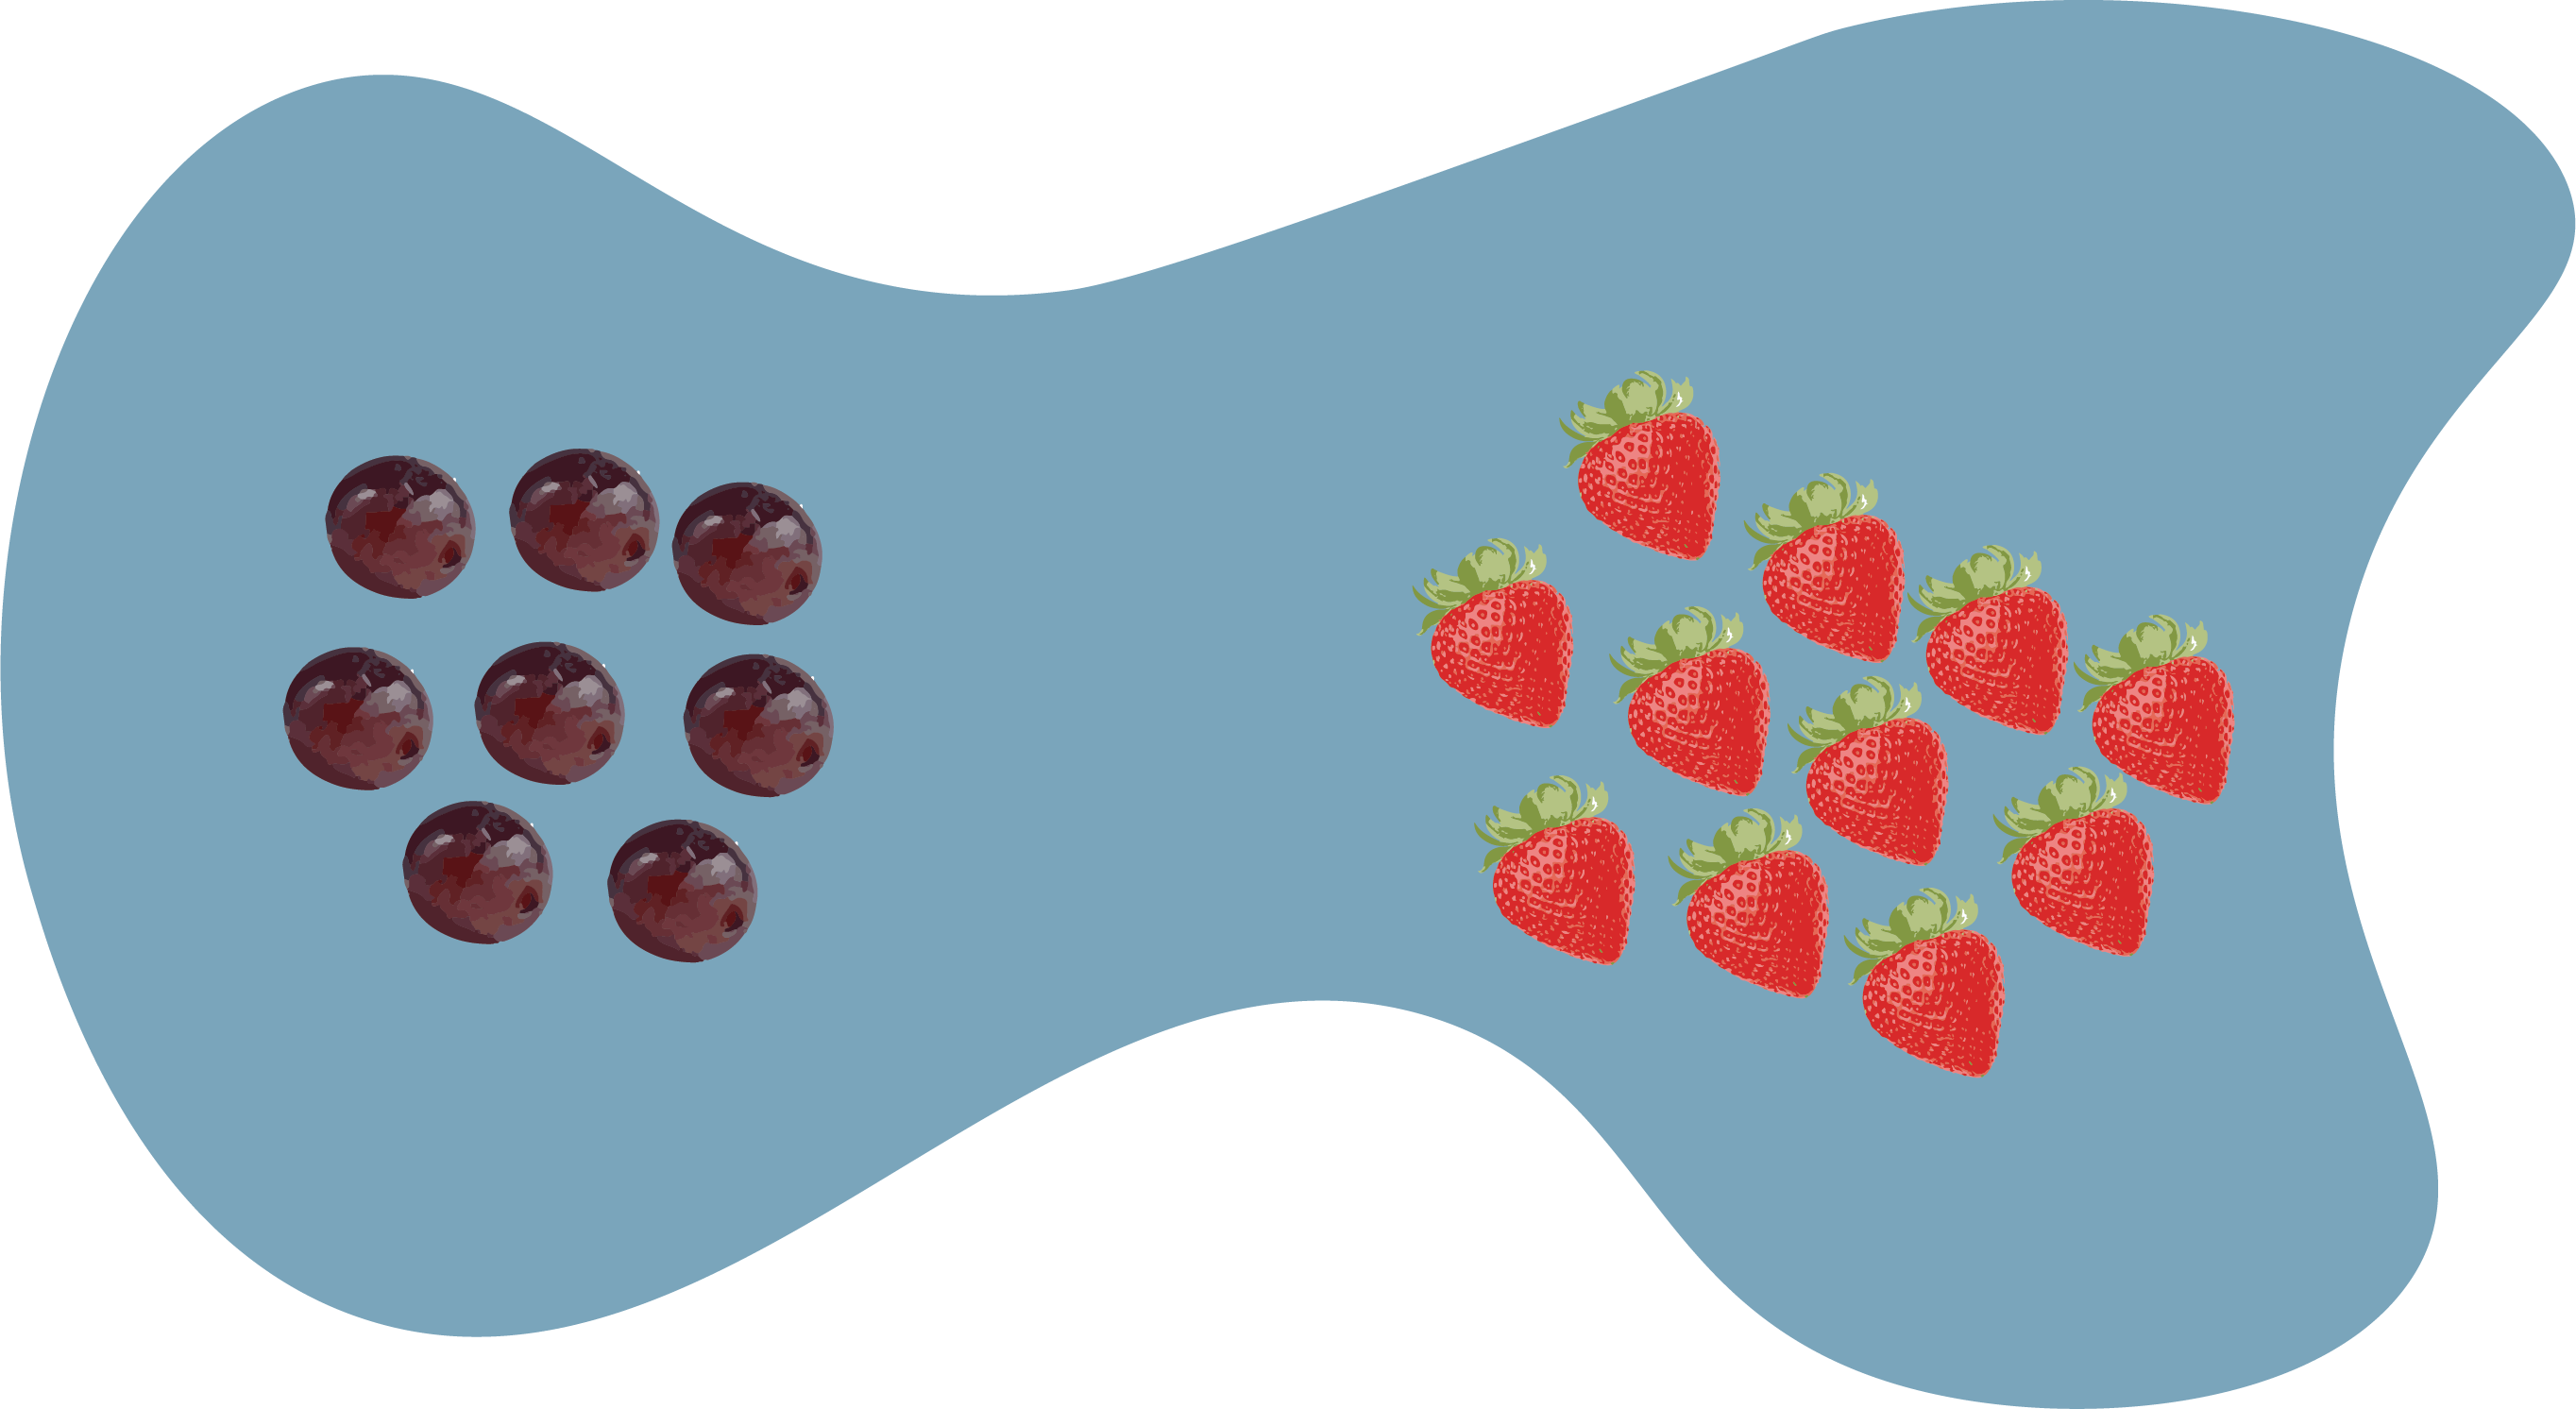
\includegraphics[width=.8\textwidth]{./media/image114.png}
\end{figure}

Somando-se as unidades de uvas e morangos que ainda serão adicionadas, podemos afirmar que ainda faltam

\begin{escolha}
\item
  25 unidades de uvas e morangos para serem adicionadas.
\item
  20 unidades de uvas e morangos para serem adicionadas.
\item
  23 unidades de uvas e morangos para serem adicionadas.
\item
  12 unidades de uvas e morangos para serem adicionadas.
\end{escolha}


\num{5} Arnaldo esqueceu um dos números que faz parte da senha do cofre que
possui em sua casa. Ele lembra que a senha era composta por 6 números e
que os números da senha formam a seguinte sequência (2, 102, 202,
\_\_A\_\_, 402, 502).
%NOTE. Ver como melhorar esse a sublinhado.

Pela análise da sequência, podemos afirmar que o número A, o qual ele esqueceu, é

\begin{multicols}{2}
\begin{escolha}
\item
  O dobro de 150.
\item
  O antecessor de 303.
\item
  O sucessor de 251.
\item
  Metade de 500.
\end{escolha}
\end{multicols}

\pagebreak
\num{6} Observando atentamente as figuras, pode-se perceber que a figura que possui a menor área é:

\begin{figure}[htpb!]
\centering
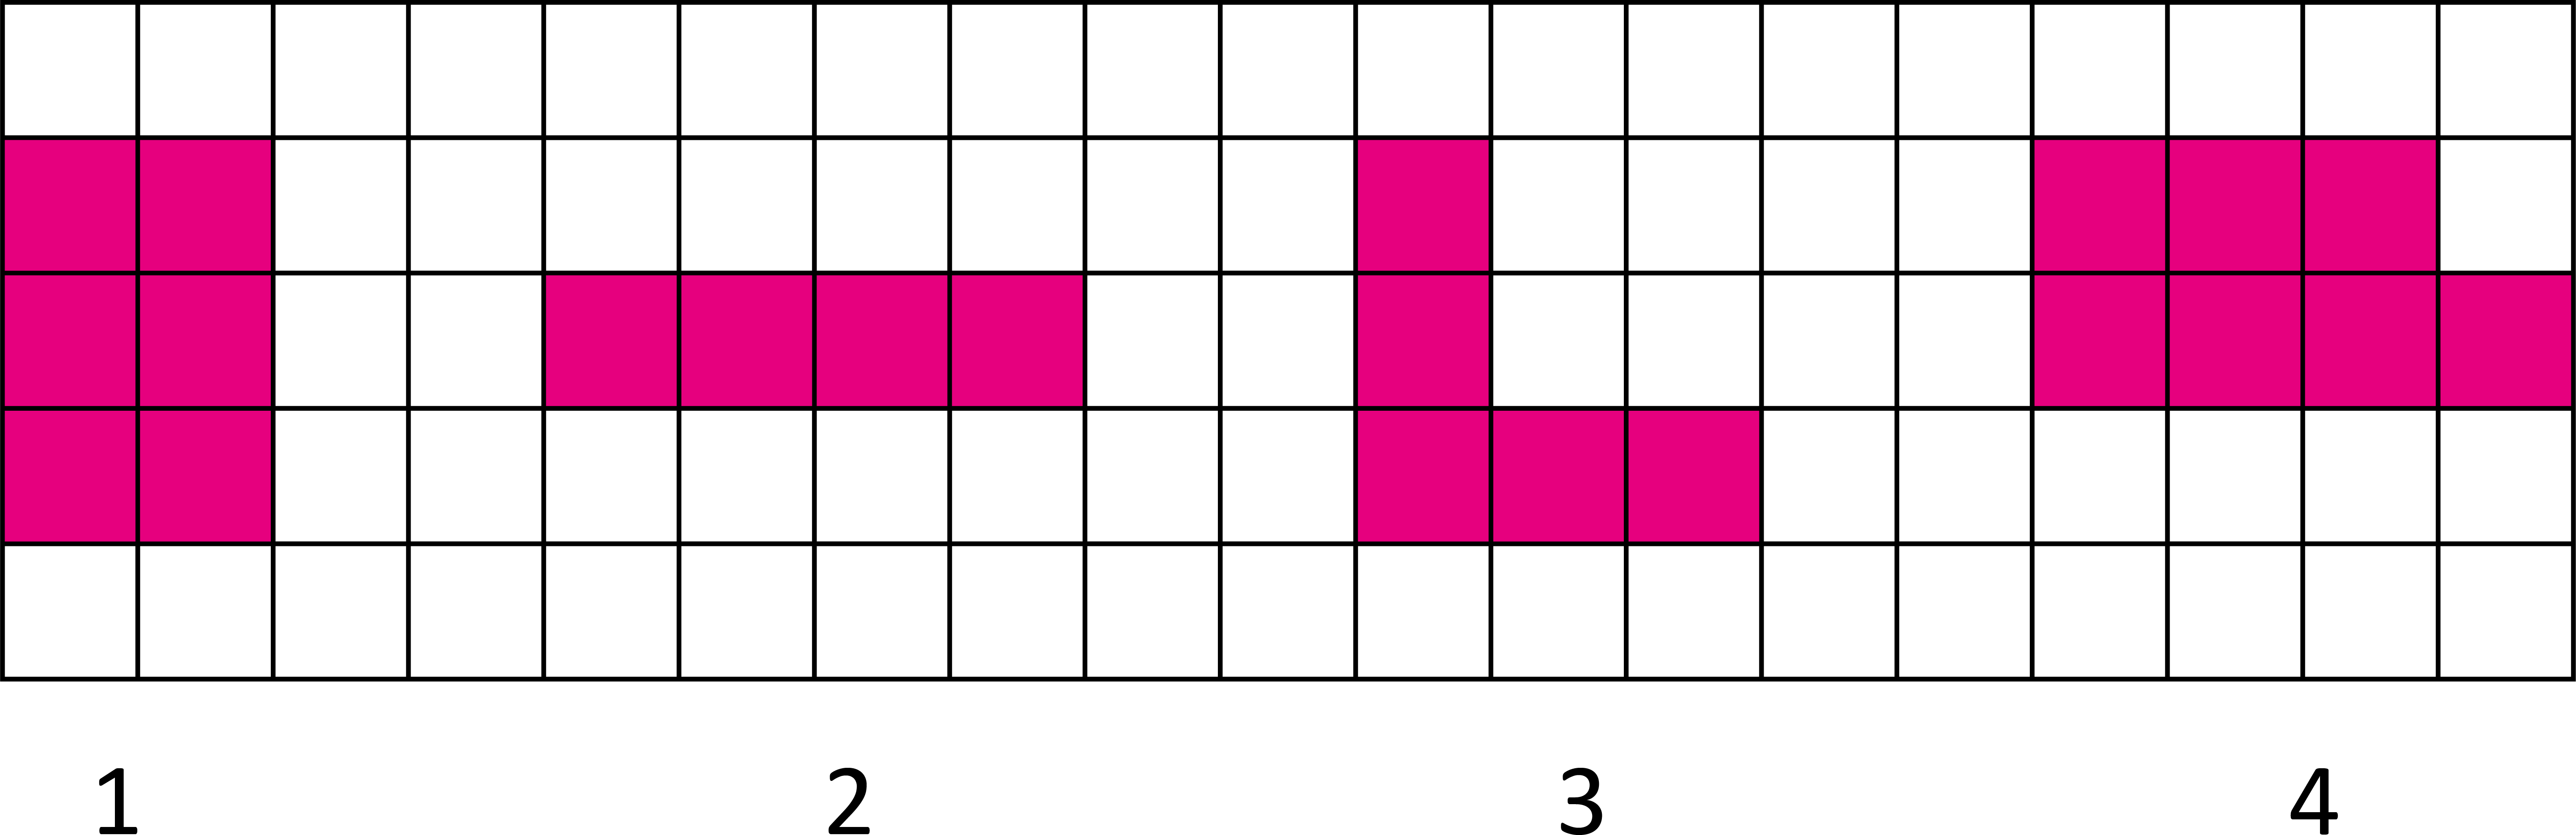
\includegraphics[width=\textwidth]{./media/image115.png}
\end{figure}

\begin{escolha}
\item
  1.
\item
  2.
\item
  3.
\item
  4.
\end{escolha}


\num{7} Maria começou a se arrumar para um passeio com suas amigas quando o relógio mostra a seguinte representação das horas:

\begin{figure}[htpb!]
\centering
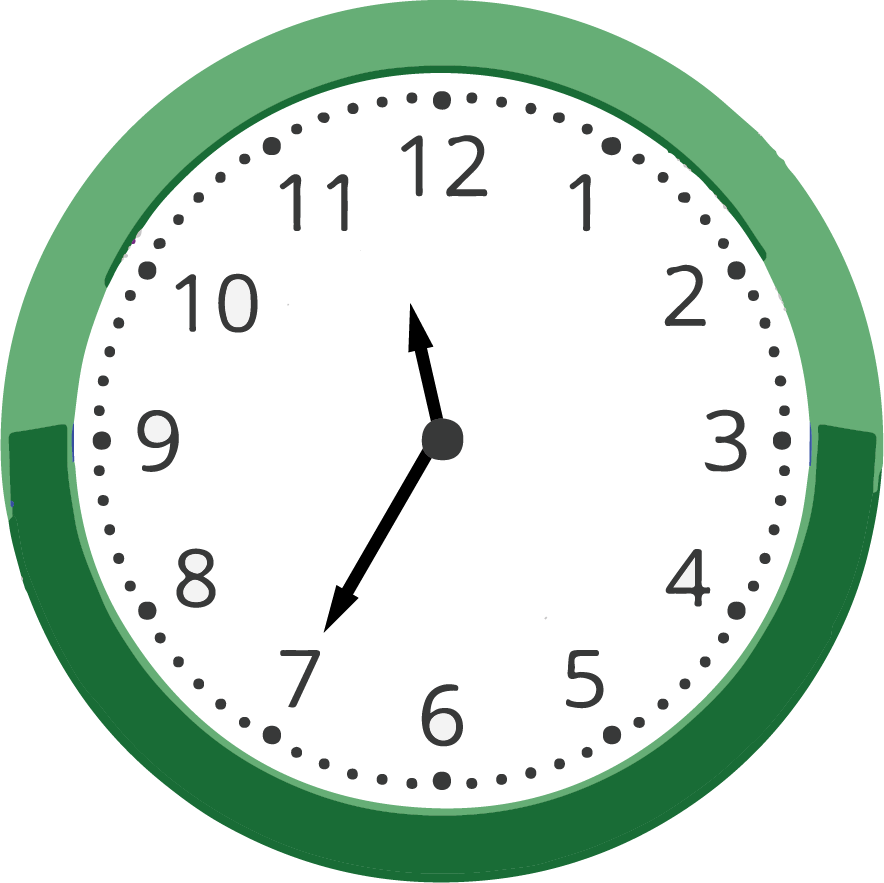
\includegraphics[width=.5\textwidth]{./media/image116.png}
\end{figure}

\pagebreak
Sabendo-se que ela terminou de se arrumar em 35 minutos, qual o horário que o relógio estava marcando quando ela terminou de se arrumar?

\begin{escolha}
\item
  11 horas e 50 minutos.
\item
  12 horas.
\item
  12 horas e 5 minutos.
\item
  12 horas e 10 minutos.
\end{escolha}


\num{8} Rafael foi a uma papelaria e comprou um livro por R\$ 35,00 e uma caneta
por R\$ 3,00. Das alternativas a seguir, qual pode representar as cédulas
e moedas que Rafael utilizou para pagar, sabendo-se que não terá troco?

\begin{escolha}

\item
  1 cédula de 10 reais, 5 cédulas de 5 reais e 3 moedas de 1 real.
\item
  1 cédula de 10 reais, 4 cédulas de 5 reais e 3 moedas de 1 real.
\item
  2 cédulas de 10 reais, 1 cédula de 5 reais e 3 moedas de 1 real.
\item
  2 cédulas de 10 reais, 2 cédulas de 5 reais e 2 moedas de 1 real.
\end{escolha}


\num{9} Alana resolveu trocar todas as moedas que estavam em seu cofrinho por uma única cédula. Ela tinha no cofrinho 10 moedas de 5 centavos, 5 moedas de
50 centavos, 70 moedas de 10 centavos.

\pagebreak
Marque a alternativa que traz a nota correta que substituiu em valor todas as moedas que Alana tinha em seu cofrinho.

\begin{figure}[htpb!]
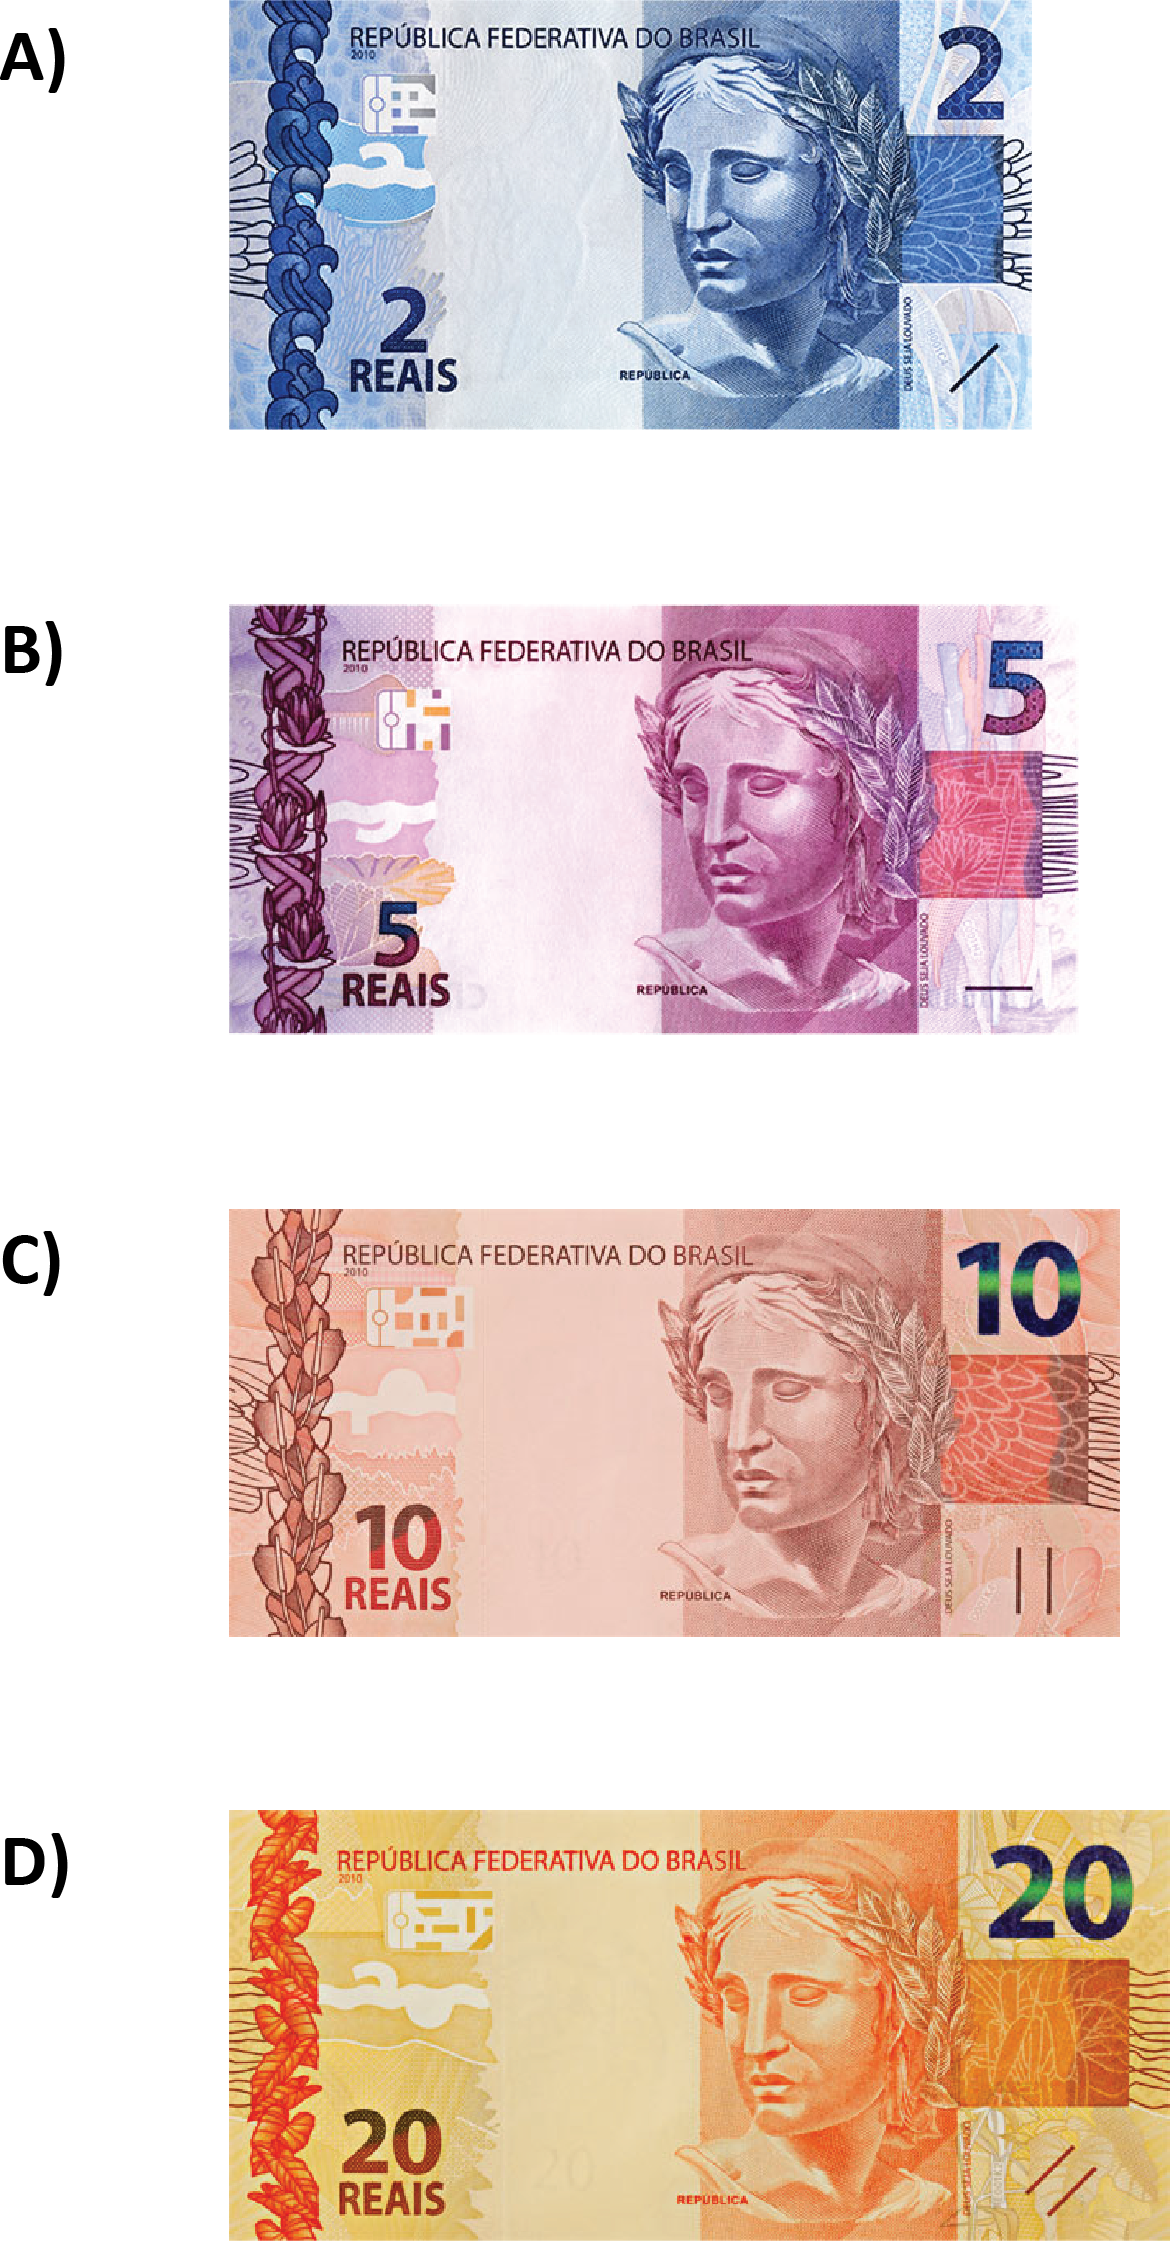
\includegraphics[width=.45\textwidth]{./media/image117.png}
\end{figure}

\num{10} O enfeite encomendado pela mãe de Joaquina para a festa de aniversário da filha era composto por 8 bexigas brancas e o triplo dessa quantidade de bexigas vermelhas. Qual é o total de bexigas presentes no enfeite?

\begin{escolha}
\item
  8.
\item
  16.
\item
  24.
\item
  32.
\end{escolha}

\num{11} Uma loja de brinquedos efetuou uma pesquisa em determinado dia para saber a faixa etária das crianças que visitaram a loja e os dados foram
colocados em um gráfico.

\begin{figure}[htpb!]
\centering
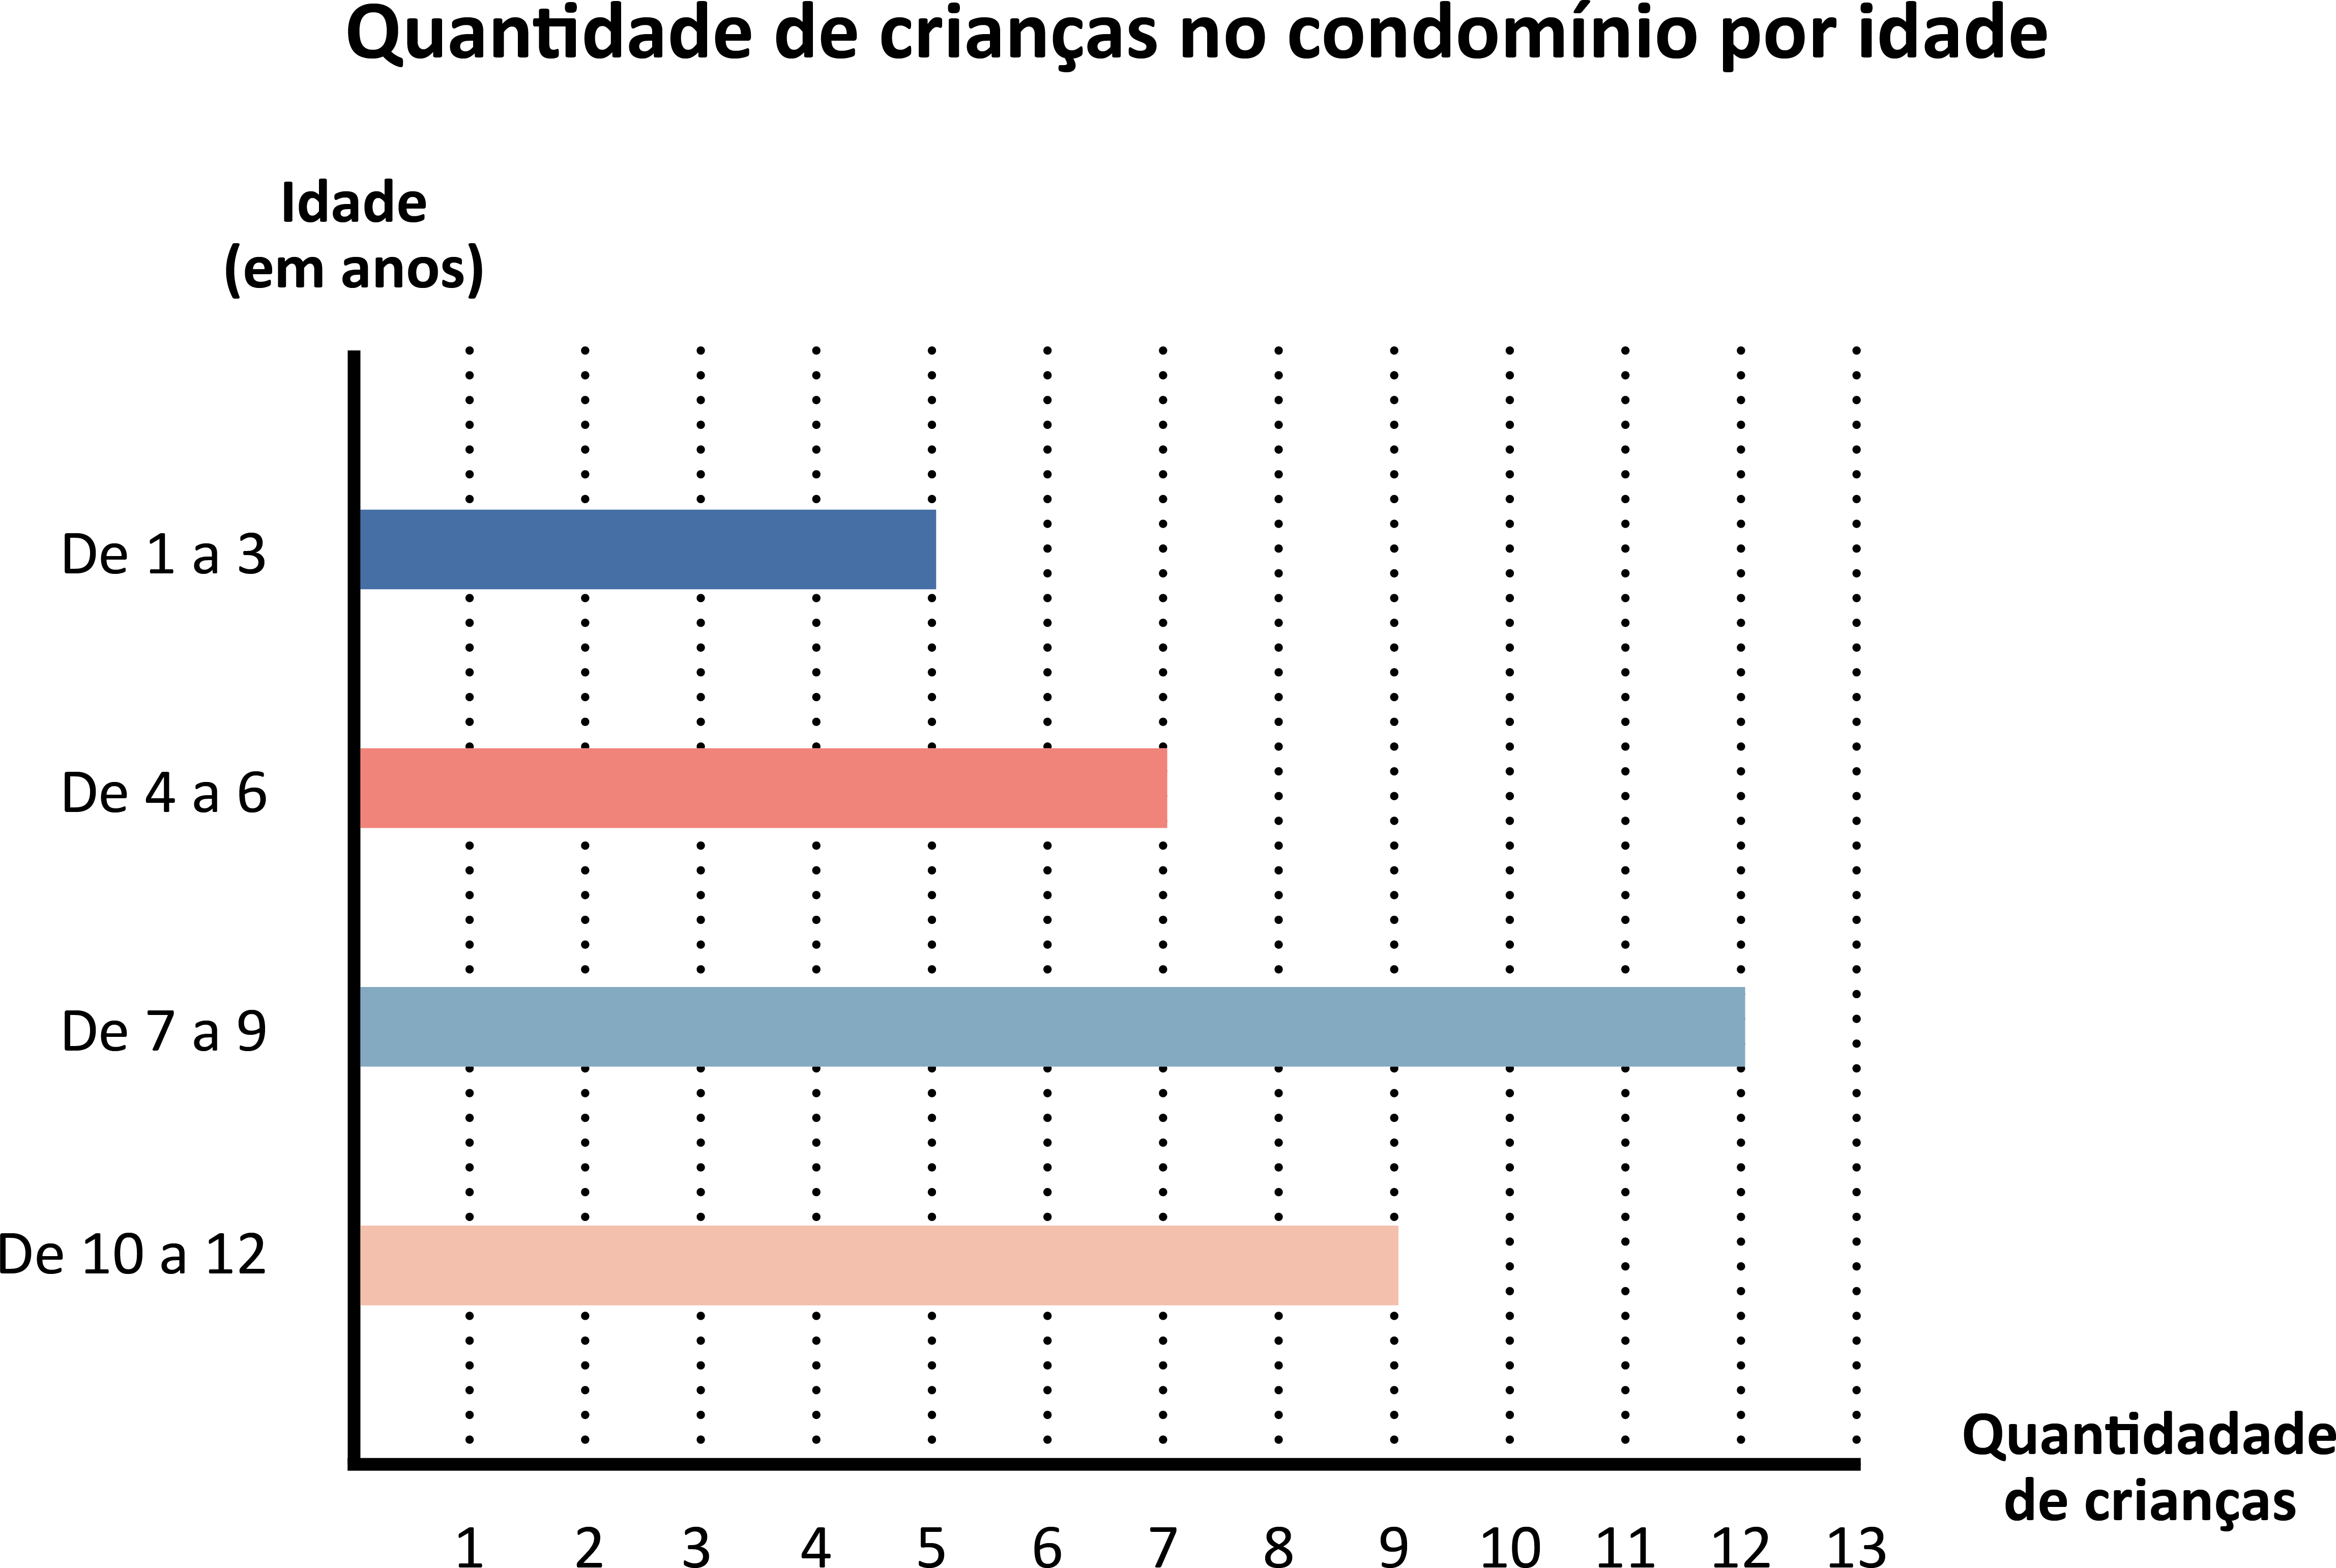
\includegraphics[width=\textwidth]{./media/image118.png}
\end{figure}

Por meio da análise do gráfico, podemos afirmar que o total de crianças de 7 a 12 anos que visitaram a loja foi de

\begin{escolha}
\item
  7.
\item
  12.
\item
  16.
\item
  21.
\end{escolha}


\pagebreak
\num{12} Um empresa de brinquedos fez um levantamento dos produtos mais vendidos e suas quantidades em um determinado mês. Esses dados foram colocados em um gráfico.


\begin{figure}[htpb!]
\centering
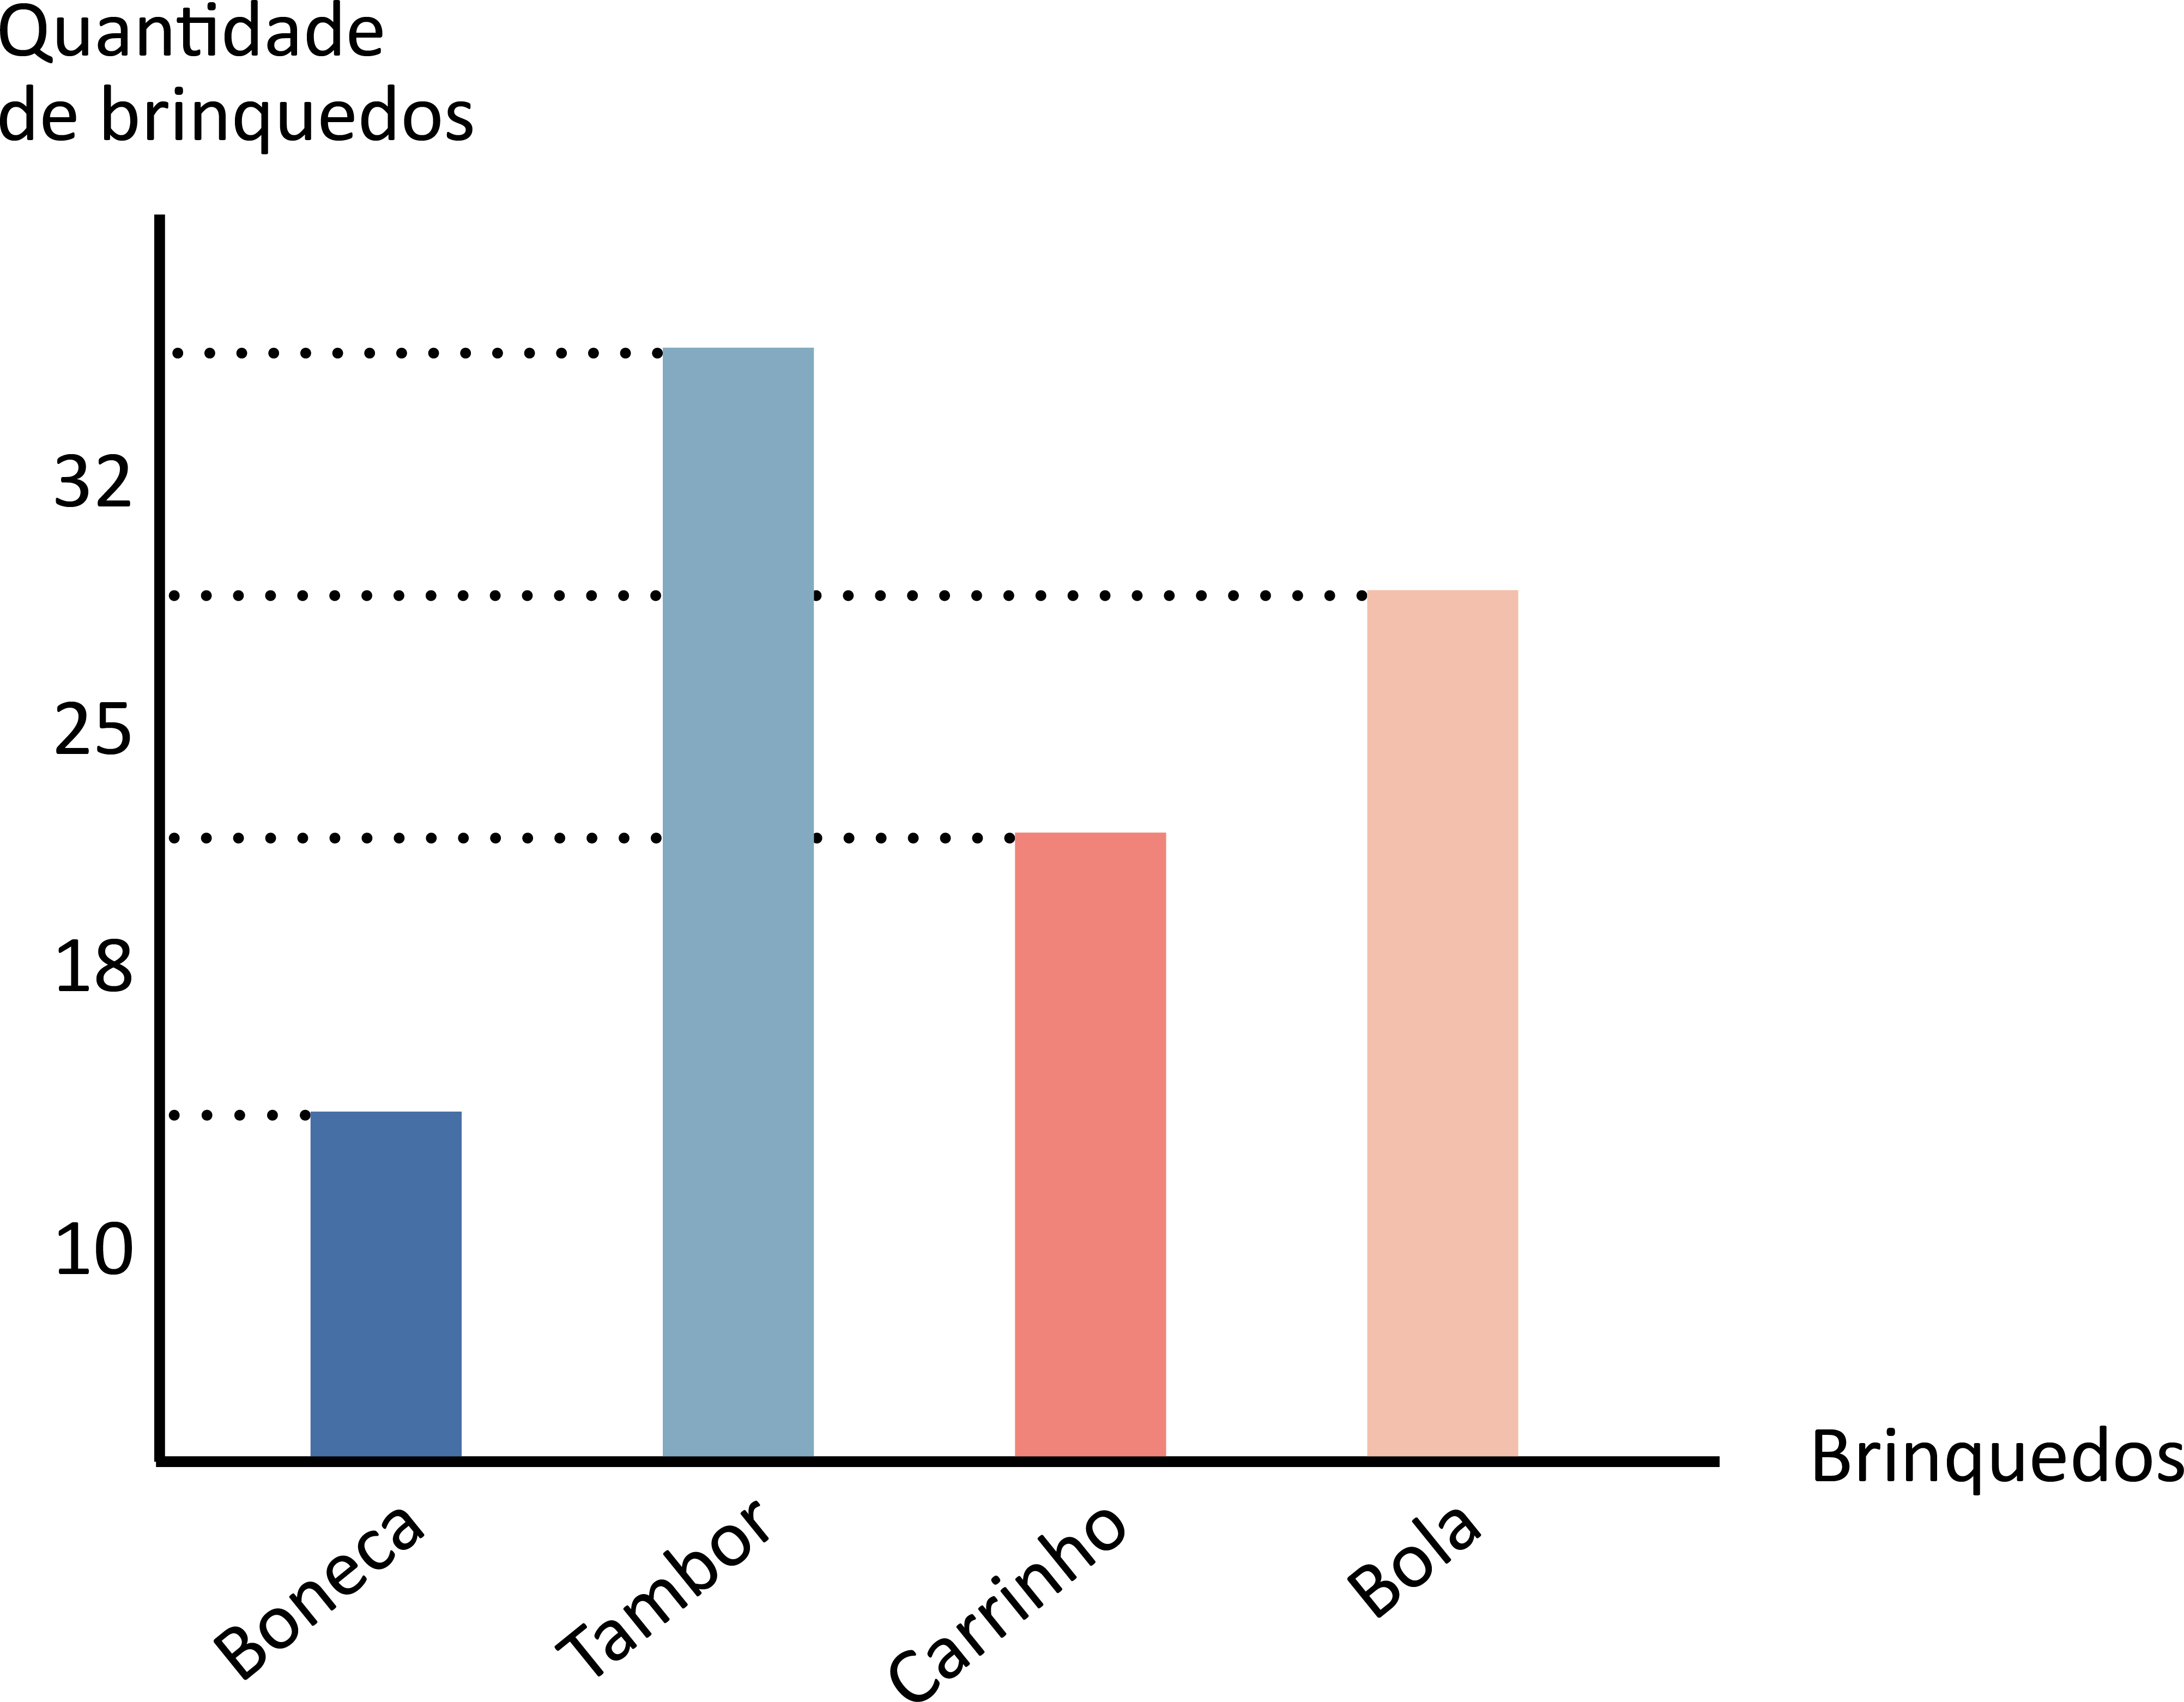
\includegraphics[width=\textwidth]{./media/image119.png}
\end{figure}

Observando o gráfico, pode-se afirmar que o produto menos vendido nesse período foi

\begin{escolha}
\item
  Boneca.
\item
  Tambor.
\item
  Carrinho.
\item
  Bola.
\end{escolha}

\pagebreak
\num{13} Observe o preço dos produtos vendidos na loja da senhora Marina:

\begin{figure}[htpb!]
\centering
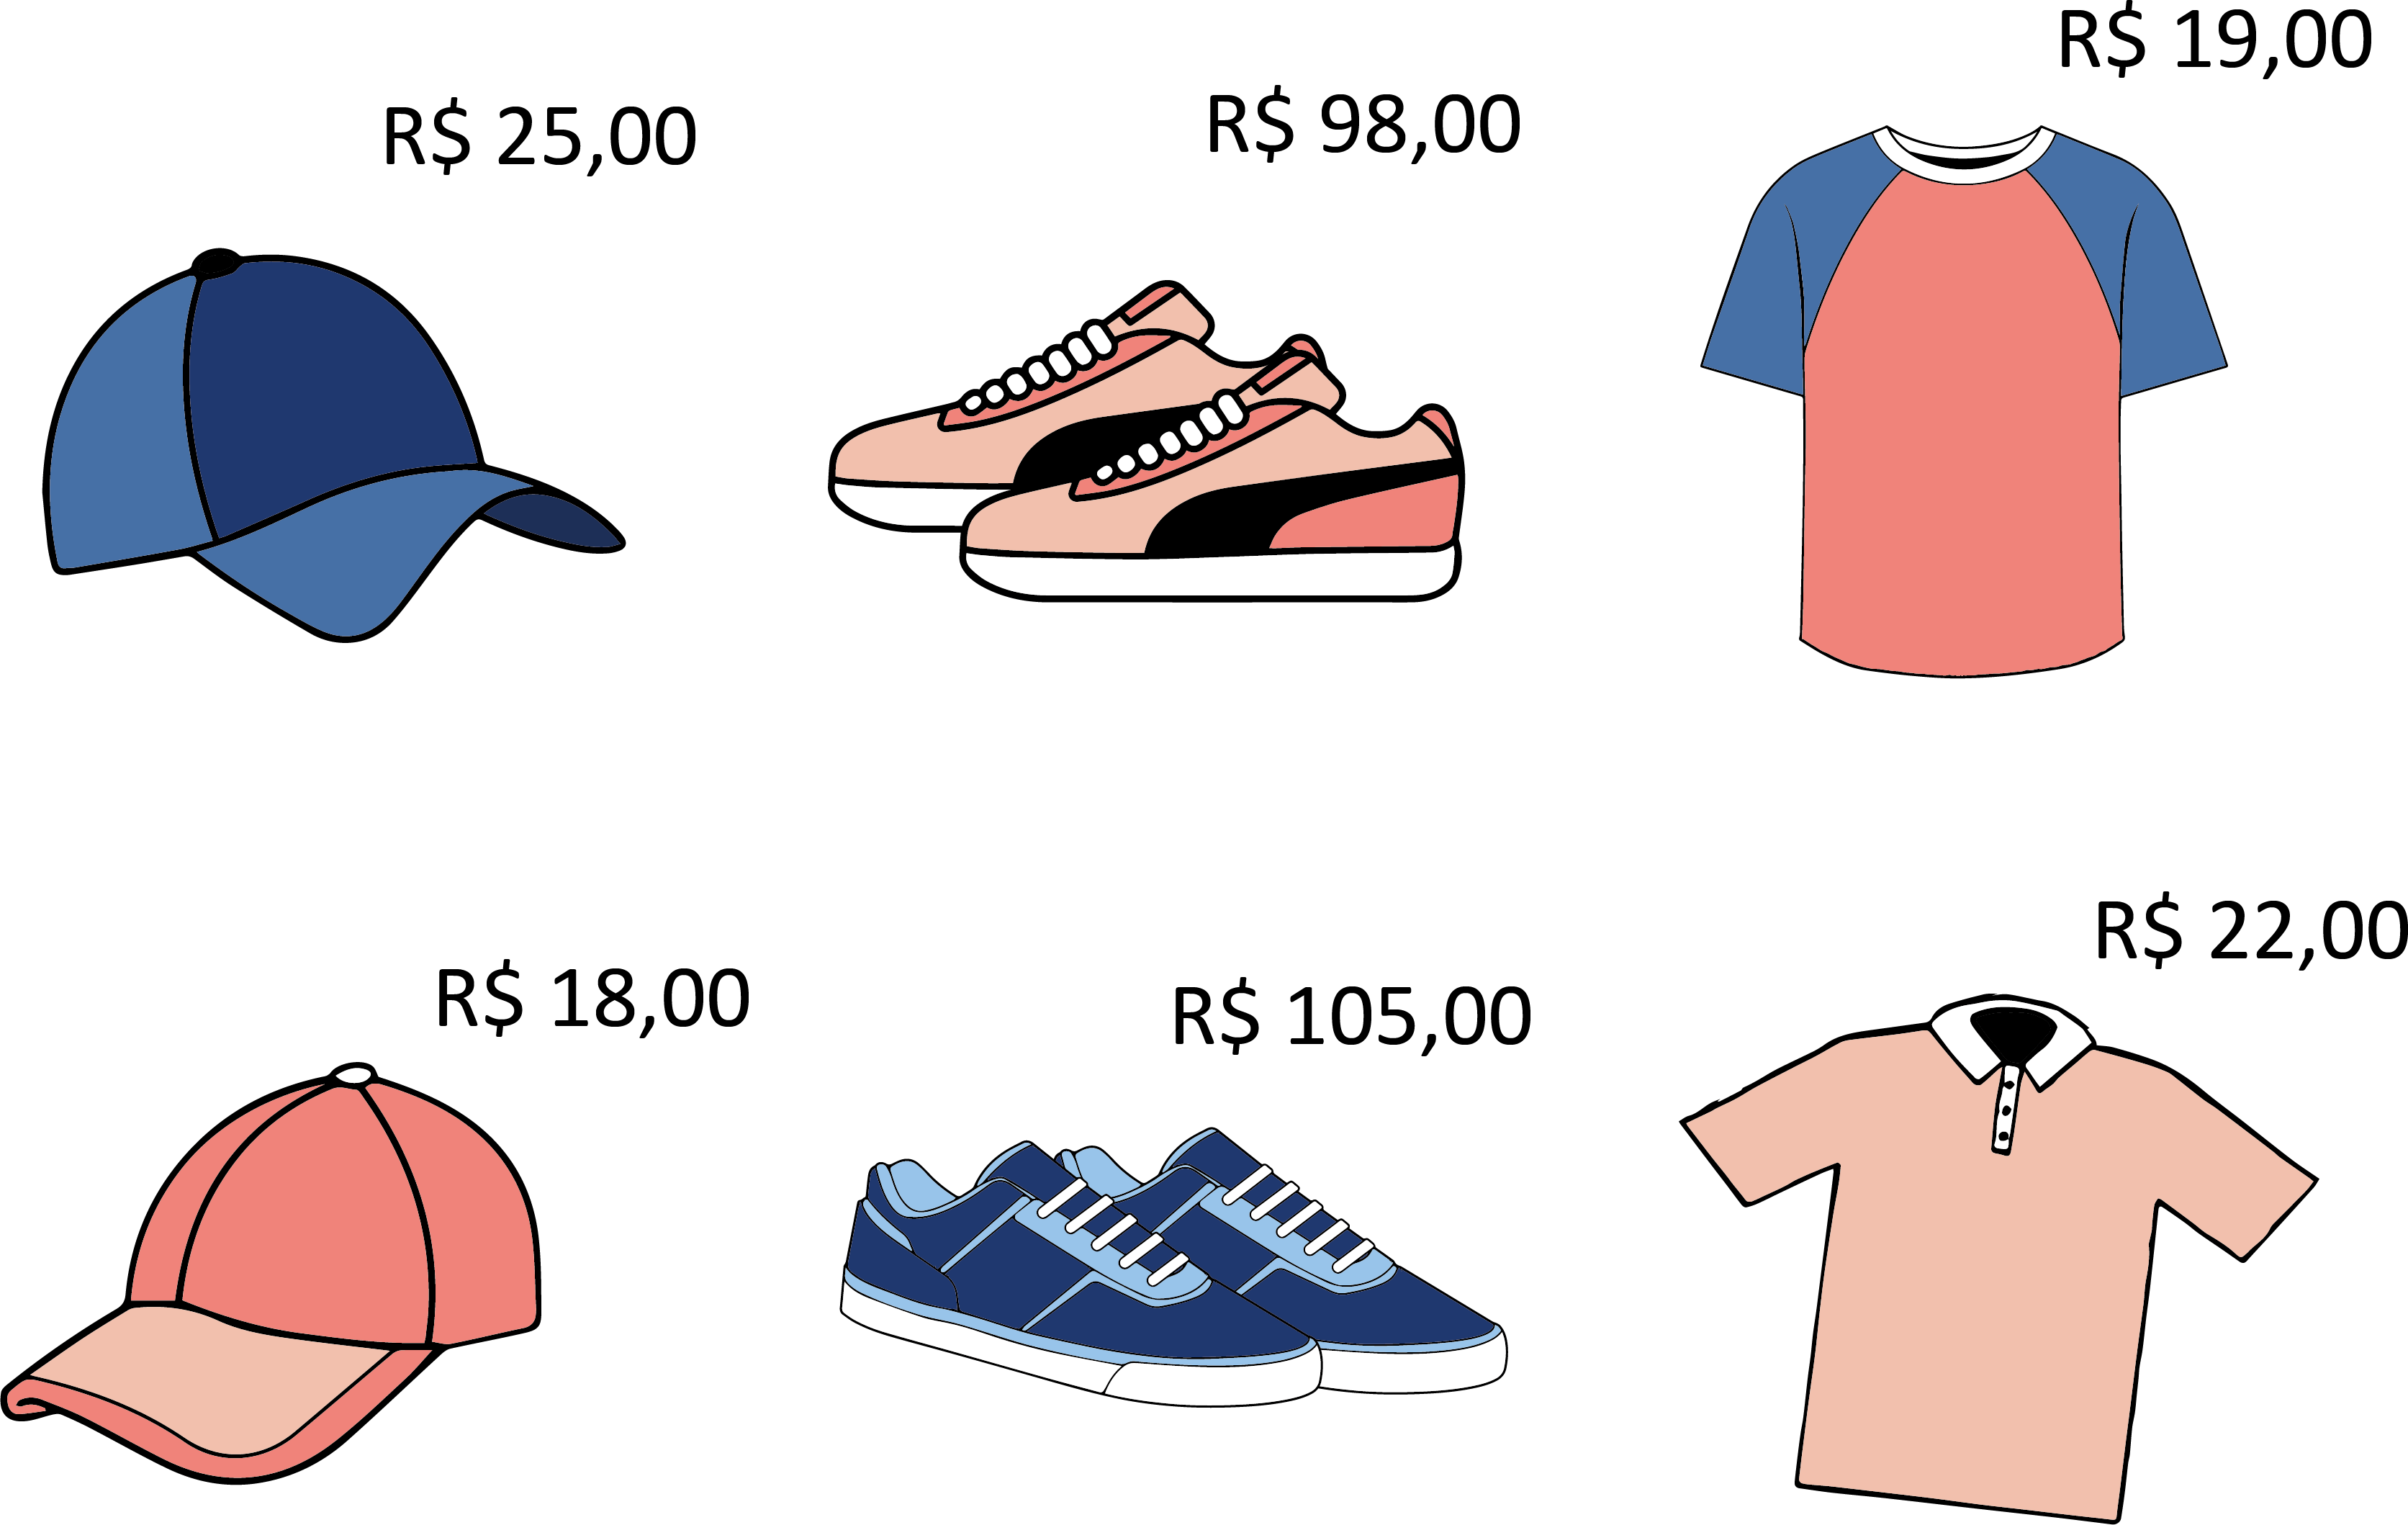
\includegraphics[width=\textwidth]{./media/image120.png}
\end{figure}

Se Alberto foi até a loja e comprou o tênis mais caro, o boné mais barato e a camiseta mais cara. Qual é o valor gasto por Alberto?

\begin{escolha}
\item
  R\$ 123,00.
\item
  R\$ 130,00.
\item
  R\$ 138,00.
\item
  R\$ 145,00.
\end{escolha}


\pagebreak
\num{14} Marcos é professor de tênis e  precisa repor o estoque de bolinhas para jogo. Para isso, ele foi até uma loja e comprou o número de embalagens indicado na figura a seguir:

\begin{figure}[htpb!]
\centering
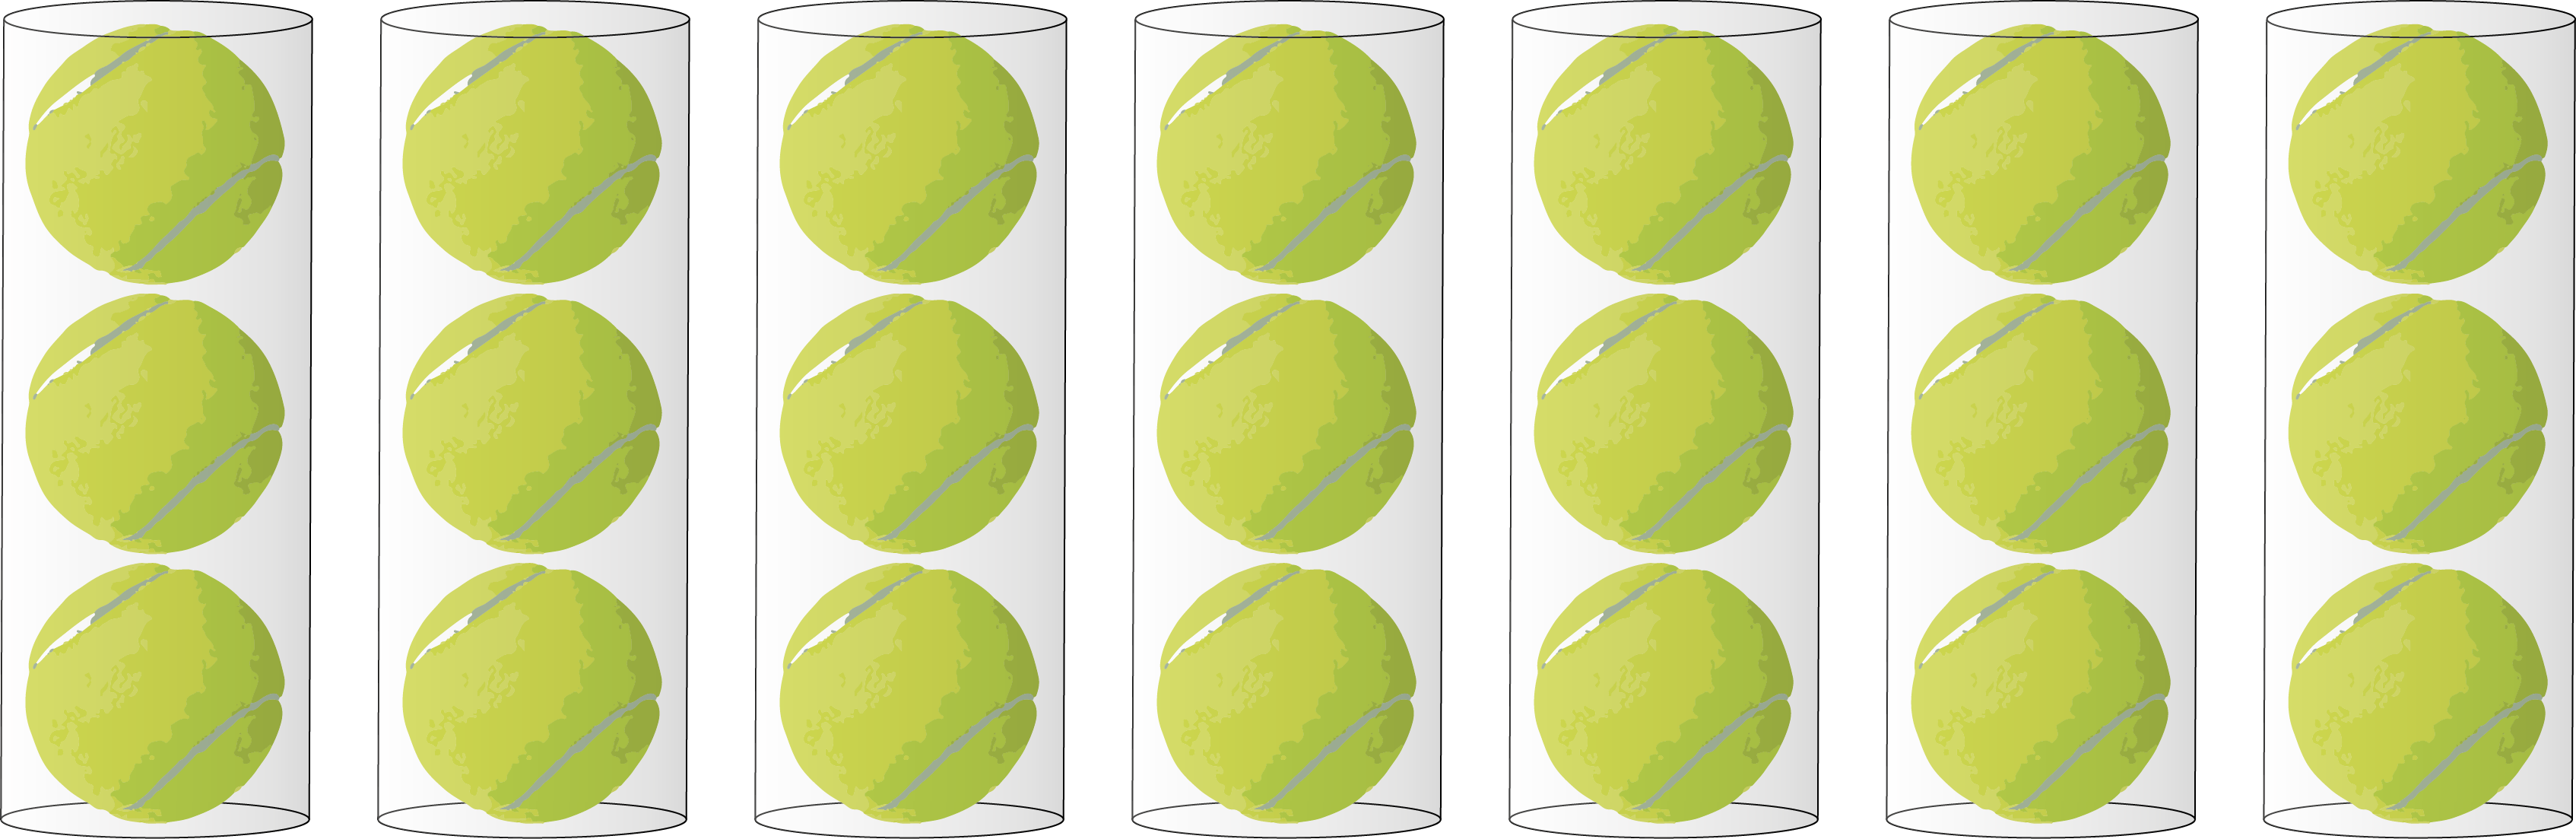
\includegraphics[width=.8\textwidth]{./media/image121.png}
\end{figure}

Pode-se afirmar que ele comprou um número de bolinhas igual a

\begin{multicols}{2}
\begin{escolha}
\item
  3.
\item
  12.
\item
  15.
\item
  21.
\end{escolha}
\end{multicols}


\num{15} Verificando algumas atividades realizadas na escola no ano anterior, Gustavo deparou-se com a seguinte conta, em que um dos números estava
coberto por um retângulo:

\begin{figure}[htpb!]
\centering  
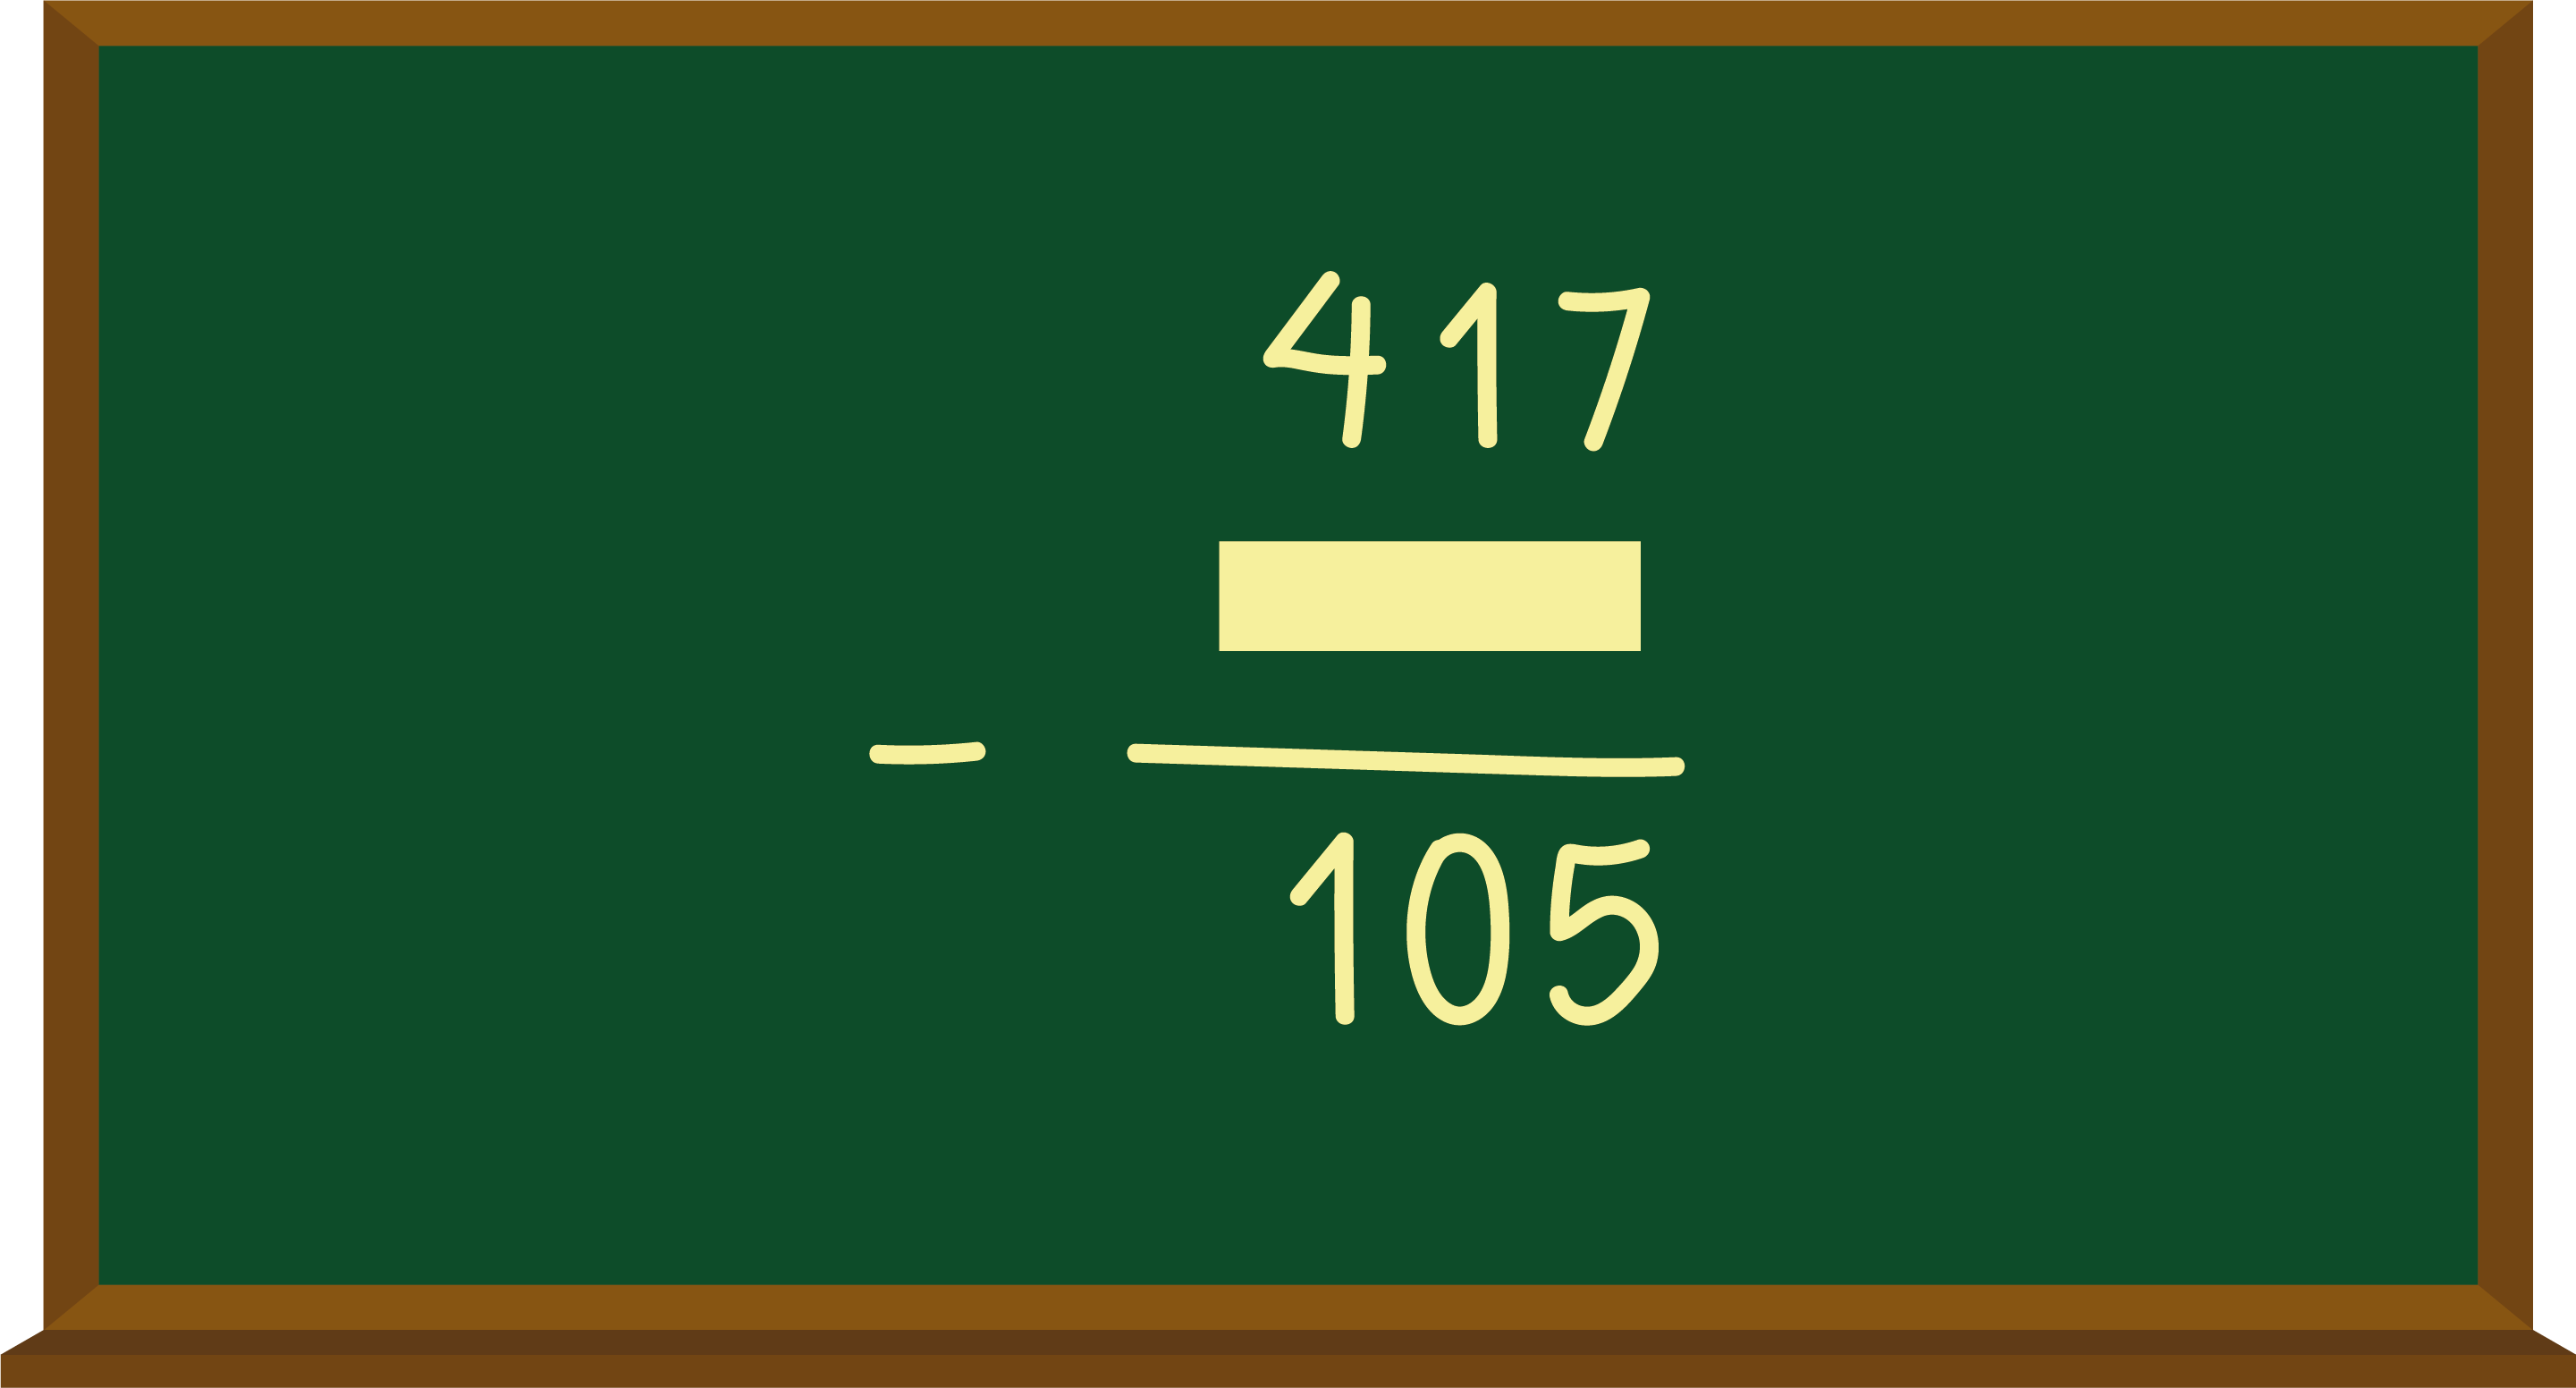
\includegraphics[width=.5\textwidth]{./media/image122.png}
\end{figure}

Gustavo ficou curioso e resolveu refazer a atividade para descobrir o número que faltava. Qual é o número que Gustavo encontrou?

\begin{multicols}{2}
\begin{escolha}
\item
  239.
\item
  312.
\item
  595.
\item
  417.
\end{escolha}
\end{multicols}



